%
%
% UCSD Doctoral Dissertation Template
% -----------------------------------
% https://github.com/ucsd-thesis/ucsd-thesis
%
%
% ----------------------------------------------------------------------
% WARNING: 
%
%   This template has not endorced by OGS or any other official entity.
%   The official formatting guide can be obtained from OGS.
%   It can be found on the web here:
%   http://grad.ucsd.edu/_files/academic-affairs/Dissertations_Theses_Formatting_Manual.pdf
%
%   No guaranty is made that this LaTeX class conforms to the official UCSD guidelines.
%   Make sure that you check the final document against the Formatting Manual.
%  
%   That being said, this class has been routinely used for successful 
%   publication of doctoral theses.  
%
%   The ucsd.cls class files are only valid for doctoral dissertations.
%
%
% ----------------------------------------------------------------------
% GETTING STARTED:
%
%   Lots of information can be found on the project wiki:
%   http://code.google.com/p/ucsd-thesis/wiki/GettingStarted
%
%
%   To make a pdf from this template use the command:
%     pdflatex template
%
%
%   To get started please read the comments in this template file 
%   and make changes as appropriate.
%
%   If you successfully submit a thesis with this package please let us
%   know.
%
%
% ----------------------------------------------------------------------
% KNOWN ISSUES:
%
%   Currently only the 12pt size conforms to the UCSD requirements.
%   The 10pt and 11pt options make the footnote fonts too small.
%
%
% ----------------------------------------------------------------------
% HELP/CONTACT:
%
%   If you need help try the ucsd-thesis google group:
%   http://groups.google.com/group/ucsd-thesis
%
%
% ----------------------------------------------------------------------
% BUGS:
%
%   Please report all bugs at:
%   https://github.com/ucsd-thesis/ucsd-thesis/issues
%
%
% ----------------------------------------------------------------------
% More control of the formatting of your thesis can be achieved through
% modifications of the included LaTeX class files:
%
%   * ucsd.cls    -- Class file
%   * uct10.clo   -- Configuration files for font sizes 10pt, 11pt, 12pt
%     uct11.clo                            
%     uct12.clo
%
% ----------------------------------------------------------------------



% Setup the documentclass 
% default options: 12pt, oneside, final
%
% fonts: 10pt, 11pt, 12pt -- are valid for UCSD dissertations.
% sides: oneside, twoside -- note that two-sided theses are not accepted 
%                            by OGS.
% mode: draft, final      -- draft mode switches to single spacing, 
%                            removes hyperlinks, and places a black box
%                            at every overfull hbox (check these before
%                            submission).
% chapterheads            -- Include this if you want your chapters to read:
%                              Chapter 1
%                              Title of Chapter
%
%                            instead of
%                              1 Title of Chapter
\documentclass[12pt,chapterheads]{ucsd}



% Include all packages you need here.  
% Some standard options are suggested below.
%
% See the project wiki for information on how to use 
% these packages. Other useful packages are also listed there.
%
%   http://code.google.com/p/ucsd-thesis/wiki/GettingStarted



%% AMS PACKAGES - Chances are you will want some or all 
%    of these if writing a dissertation that includes equations.
%  \usepackage{amsmath, amscd, amssymb, amsthm}

%% BONUS MATH
%  \usepackage{mathtools} 

%% MARGIN REQUIREMENTS IN TITLES - Hyphenation in a Section Title does not always respect margin settings in Latex.  To force no hyphentation, uncomment the package below.
%  \usepackage[raggedright]{titlesec} 

%% GRAPHICX - This is the standard package for 
%    including graphics for latex/pdflatex.
\usepackage{scrextend}
\usepackage{pslatex}
\usepackage{graphicx}

%% CAPTION
% This overrides some of the ugliness in ucsd.cls and
% allows the text to be double-spaced while letting figures,
% tables, and footnotes to be single-spaced--all OGS requirements.
% NOTE: Must appear after graphics and ams math
\makeatletter
\gdef\@ptsize{2}% 12pt documents
\let\@currsize\normalsize
\makeatother
\usepackage{setspace}
\doublespace
\usepackage[font=small, width=0.9\textwidth]{caption}

%% SUBFIG - Use this to place multiple images in a
%    single figure.  Subfig will handle placement and
%    proper captioning (e.g. Figure 1.2(a))
% \usepackage{subfig}

%% TIMES FONT - replacements for Computer Modern
%%   This package will replace the default font with a
%%   Times-Roman font with math support.
% \usepackage[T1]{fontenc}
% \usepackage{mathptmx}

%% INDEX
%   Uncomment the following two lines to create an index: 
% \usepackage{makeidx}
% \makeindex
%   You will need to uncomment the \printindex line near the
%   bibliography to display the index.  Use the command
% \index{keyword} 
%   within the text to create an entry in the index for keyword.
%   To compile a LaTeX document with an index the 'makeindex'
%   command will need to be run.  See the wiki for more details.

%% HYPERLINKS
%   To create a PDF with hyperlinks, you need to include the hyperref package.
%   THIS HAS TO BE THE LAST PACKAGE INCLUDED!
%   Note that the options plainpages=false and pdfpagelabels exist
%   to fix indexing associated with having both (ii) and (2) as pages.
%   Also, all links must be black according to OGS.
%   See: http://www.tex.ac.uk/cgi-bin/texfaq2html?label=hyperdupdest
%   Note: This may not work correctly with all DVI viewers (i.e. Yap breaks).
%   NOTE: hyperref will NOT work in draft mode, as noted above.
% \usepackage[colorlinks=true, pdfstartview=FitV, 
%             linkcolor=black, citecolor=black, 
%             urlcolor=black, plainpages=false,
%             pdfpagelabels]{hyperref}
% \hypersetup{ pdfauthor = {Your Name Here}, 
%              pdftitle = {The Title of The Dissertation}, 
%              pdfkeywords = {Keywords for Searching}, 
%              pdfcreator = {pdfLaTeX with hyperref package}, 
%              pdfproducer = {pdfLaTeX} }
% \urlstyle{same}
% \usepackage{bookmark}


%% CITATIONS
% Sets citation format
% and fixes up citations madness
\usepackage{microtype}  % avoids citations that hang into the margin


%% FOOTNOTE-MAGIC
% Enables footnotes in tables, re-referencing the same footnote multiple times.
\usepackage{footnote}
\makesavenoteenv{tabular}
\makesavenoteenv{table}


%% TABLE FORMATTING MADNESS
% Enable all sorts of fun table tricks
\usepackage{rotating}  % Enables the sideways environment (NCPW)
\usepackage{array}  % Enables "m" tabular environment http://ctan.org/pkg/array
\usepackage{booktabs}  % Enables \toprule  http://ctan.org/pkg/array



\begin{document}

%% FRONT MATTER
%
%  All of the front matter.
%  This includes the title, degree, dedication, vita, abstract, etc..
%  Modify the file template_frontmatter.tex to change these pages.
%
%
% UCSD Doctoral Dissertation Template
% -----------------------------------
% http://ucsd-thesis.googlecode.com
%
%


%% REQUIRED FIELDS -- Replace with the values appropriate to you

% No symbols, formulas, superscripts, or Greek letters are allowed
% in your title.
\title{Interactive Attunement Catalyzes Creative Learning}

\author{Tricia J. Ngoon}
\degreeyear{\the\year}

% Master's Degree theses will NOT be formatted properly with this file.
\degreetitle{Doctor of Philosophy}

\field{Cognitive Science}

\chair{Scott R. Klemmer}
% Uncomment the next line iff you have a Co-Chair
% \cochair{Professor Cochair Semimaster}
%
% Or, uncomment the next line iff you have two equal Co-Chairs.
%\cochairs{Professor Chair Masterish}{Professor Chair Masterish}

%  The rest of the committee members  must be alphabetized by last name.
\othermembers{
Steven P. Dow\\
William G. Griswold\\
Philip J. Guo\\
Joy O. Kim\\
Caren M. Walker
}
\numberofmembers{6} % |chair| + |cochair| + |othermembers|


%% START THE FRONTMATTER
%
\begin{frontmatter}

%% TITLE PAGES
%
%  This command generates the title, copyright, and signature pages.
%
\makefrontmatter

%% DEDICATION
%
%  You have three choices here:
%    1. Use the ``dedication'' environment.
%       Put in the text you want, and everything will be formated for
%       you. You'll get a perfectly respectable dedication page.
%
%
%    2. Use the ``mydedication'' environment.  If you don't like the
%       formatting of option 1, use this environment and format things
%       however you wish.
%
%    3. If you don't want a dedication, it's not required.
%
%
\begin{dedication}
  To my parents. Thank you.
\end{dedication}


% \begin{mydedication} % You are responsible for formatting here.
%   \vspace{1in}
%   \begin{flushleft}
% 	To me.
%   \end{flushleft}
%
%   \vspace{2in}
%   \begin{center}
% 	And you.
%   \end{center}
%
%   \vspace{2in}
%   \begin{flushright}
% 	Which equals us.
%   \end{flushright}
% \end{mydedication}



%% EPIGRAPH
%
%  The same choices that applied to the dedication apply here.
%
\begin{epigraph} % The style file will position the text for you.
  \emph{To know, is to know that you know nothing.\\
  That is the meaning of true knowledge.}\\
  ---Socrates
\end{epigraph}

% \begin{myepigraph} % You position the text yourself.
%   \vfil
%   \begin{center}
%     {\bf Think! It ain't illegal yet.}
%
% 	\emph{---George Clinton}
%   \end{center}
% \end{myepigraph}


%% SETUP THE TABLE OF CONTENTS
%
\tableofcontents
\listoffigures  % Comment if you don't have any figures
\listoftables   % Comment if you don't have any tables



%% ACKNOWLEDGEMENTS
%
%  While technically optional, you probably have someone to thank.
%  Also, a paragraph acknowledging all coauthors and publishers (if
%  you have any) is required in the acknowledgements page and as the
%  last paragraph of text at the end of each respective chapter. See
%  the OGS Formatting Manual for more information.
%
\begin{acknowledgements}
    Six years and more than ten existential crises later, I've finally finished this thing that we call a PhD. Doing a PhD is not an easy journey, especially during a global pandemic. I certainly could not have achieved this feat without the help of so many amazing people in my life. This is my attempt to show my immense appreciation and gratitude to all those who have led me to this accomplishment.
 
Thank you to my committee -- Scott, Caren, Joy, Steven, Bill, and Philip -- for your endless support and feedback. In particular, thank you Scott for being my biggest advocate and pushing me to be a better researcher and thinker. I never would have thought that taking your Interaction Design course on Coursera would lead to me applying to UCSD almost on a whim. I am so grateful that you saw and continue to see potential in me. Thank you to Caren for being such a big influence in my research and a true inspiration. Thank you Joy for being an amazing mentor and welcoming me into the Adobe Research family. Thank you Philip for always checking in and providing me with encouragement. Thank you Steven for the fruitful research discussions and feedback. Thank you Bill for your stimulating discussions and questions during lab meeting and your constant encouragement. 
 
I am blessed to have incredible research collaborators, colleagues, and research assistants. Thank you Adobe Research for giving me opportunities to expand my research, and especially to Mira Dontcheva for all your wonderful feedback and advice through our collaborations. Thank you Michelle Lee, Nicolas La Polla, and Vivian Leung for being such bright and hard-working RAs. This research would not have been possible without your dedication. I am especially proud of Vivian for completing a wonderfully written undergrad thesis on our work together. Thank you Design Lab grad students for creating a supportive and collegial environment within the lab. Thank you to the extended HCI research community and all the people I have had the pleasure of meeting at conferences. In particular, thank you Eunice for being an awesome C\&C Student Volunteer Co-Chair and allowing me to share your hotel room when I was stranded in Austin during CSCW. Thank you Yea-Seul for being a fellow ``Rising Star'' with me and extensive discussions about our futures after grad school. Thank you Grace for all the insightful conversations interning together at Adobe. Thank you Minsuk for always being a friendly face at conferences. Thank you Jane for all the productive ``work’’ sessions. You have truly been a positive influence on my research and mental health, and I'm a little sad that we won't get to collaborate together at UCSD. Going further back, I am thankful for Tanya Evans’s and Christian Batista's mentorship during my time at Stanford. My interest in research all stemmed from Art Shimamura's Learning \& Memory class, and I am grateful for his guidance in completing my senior thesis with him.
 
I am also grateful for the Design Lab and the Cognitive Science Department. Thank you Olga, Sara, Vanessa, Ian, and Michel\'{e} for welcoming me into the Design Lab with open arms. Thank you Teenah Eco for being the first person I met in the lab and always being a smiling and friendly presence. Thank you Colleen for frequently checking in on how my family was doing. Thank you to Don Norman for being supportive of everyone in the lab and providing insightful feedback throughout my time here. Thank you Beverley for being the British grandmother I never had and always lending a supportive ear. Thank you Ethel for all your help in getting me to the finish line. Thank you Thanh for supporting me and the rest of the department through all your hard work. Thank you Marta Kutas and Andrea Chiba for helping build my formative research years through my 2nd and 3rd year projects. Thank you Drew Walker for being an advocate for TAs and helping me grow as an instructor. Thank you Doug Nitz and Eran Mukamel for standing up for CogSci grad students when we needed it most.
 
A huge amount of gratitude goes out to my support crew of friends. Thank you to the crewtons for all the sushiboocha and other shenanigans. Thank you to my tiny, but mighty MARKETS cohort (Michael, Amy, Reina, Kevin, Eric, and Shuai) for having each others' backs all these years. Amy, I remember being roommates with you when we first interviewed at UCSD, and I'm so glad we both ended up here and remained such close friends. Ailie, my two-time award-winning co-author, awkward travel buddy, and awesome friend, thank you for all your support both in research and general life. Vineet, thank you for being a shining example of passionate, hard work and for sending your wonderful Friday clips. Thank you to all my past officemates (Ariel, Julia, Sam, Srishti, Matin, Nida, and Yasmine) for making our tiny closet office more bearable. Thank you Ariana for being such an understanding and strong person in my life and pushing me to be more assertive and social. Thank you Janet for being a fun adventure friend and discussing all things Marvel with me. Thank you Chris for being a fellow awkward friend even though I yell at you a lot (deservedly). To my roommate Rob, thank you for making life infinitely more loud and interesting. Robercia Junction will live on forever. Thank you Vicky, Kenny, and Zoe for being great travel buddies and for all the fun movie nights. Thank you Gio for inspiring a lot of my thoughts about coaching and creativity. Thank you Jocelyn for remaining one of my closest friends and a constant source of positivity over the years. Thank you Calvin for remaining a supportive figure in my life even at a distance and being my sounding board for ranting. Thank you to my extended Wushu family who I know I can always count on even if we're worlds apart. Thank you to the rest of the Fab 4 (Paola, Sandhya, and Sally) for your inspiration and friendship. You are all doing such amazing things. 
 
Finally, I would like to give the biggest thank you to my extended and immediate family for their unconditional love and support. To Lynn, you are more like a sister than a cousin to me. We are the same type of weird, and I am thankful we've been so close for our entire lives. To George, you have always been family to me. You are now stuck with putting up with Lynn and me together forever. To Jessica, we don't see each other often, but I'm proud of the people we have both become. To my big brother Chris, I've truly enjoyed seeing our relationship improve to where we can watch game shows, travel, and laugh at a hundred inside jokes together. To my mother and father Josephine and Peter, thank you for always being a strong influence in my success. This dissertation is dedicated to you, and I hope to continue to make you proud.
\\

\textsc{Chapter \ref{chapter:abstraction}}, in part, is currently being prepared for submission for publication of the material by Tricia J. Ngoon, Joy O. Kim, and Scott Klemmer. The dissertation author was the primary investigator and author of this material.

\textsc{Chapter \ref{chapter:shown}}, in part, includes  portions of material as it appears in \textit{Sh\"{o}wn: Adaptive Conceptual Guidance Aids Example Use in Creative Tasks} by Tricia  J. Ngoon, Joy O. Kim, and Scott Klemmer in the Proceedings of the 2021 ACM Conference on Designing Interactive Systems (DIS '21). The dissertation author was the primary investigator and author of this paper.

\textsc{Chapter \ref{chapter:critiquekit}}, in part, includes portions of material as it appears in \textit{Interactive Guidance Techniques for Improving Creative Feedback} by Tricia J. Ngoon, C. Ailie Fraser, Ariel S. Weingarten, Mira Dontcheva, and Scott Klemmer in the Proceedings of the 2018 ACM Conference on Human Factors in Computing Systems (CHI '18). The dissertation author was one of the primary investigators and authors of this paper.

\textsc{Chapter \ref{chapter:future}}, in part, is currently being prepared for submission for publication of the material by Tricia J. Ngoon, Vivian Leung, and Caren M. Walker. The dissertation author was the primary investigator and author of this material.

\textsc{Chapter \ref{chapter:future}}, in part, includes portions of material as it appears in \textit{The Dark Side of Satisficing: Setting the Temperature of Creative Thinking} by Tricia J. Ngoon, Caren M. Walker, and Scott Klemmer in the Proceedings of the 2019 ACM Conference on Creativity and Cognition (C\&C '19). The dissertation author was the primary investigator and author of this material.

% \textsc{Chapter \ref{chapter:future}}, in part, includes portions of material as it appears in the paper in submission \textit{Constructive Activities for Supporting People's Creative Scientific Insights} by Vineet Pandey, Tricia J. Ngoon, and Samuel Lau. The dissertation author is an author of this paper.
\end{acknowledgements}


%% VITA
%
%  A brief vita is required in a doctoral thesis. See the OGS
%  Formatting Manual for more information.
%
\begin{vitapage}
    \begin{vita}
  \item[2013] B.~A. in Psychology with Honors, University of California Berkeley
  \item[2018] M.~S. in Cognitive Science, University of California San Diego
  \item[2021] Ph.~D. in Cognitive Science, University of California San Diego
\end{vita}
\begin{publications}
%   \item Tricia J. Ngoon, Joy O. Kim, \& Scott Klemmer. Thinking  with Boxes: Tools for Abstraction Enable Flexible Creative Work. In submission.
  \item Tricia J. Ngoon, Joy O. Kim, \& Scott Klemmer. Sh\"{o}wn: Adaptive Conceptual Guidance Aids Example Use in Creative Tasks. 2021. To appear in \textit{Proceedings of the 2021 Conference on Designing Interactive Systems (DIS '21)}.
  \item C. Ailie Fraser, Tricia J. Ngoon, Mira Dontcheva, and Scott Klemmer. 2019. RePlay: Contextually Presenting Learning Videos Across Software Applications. In \textit{Proceedings of the 2019 CHI Conference on Human Factors in Computing Systems (CHI '19)}. Association for Computing Machinery, New York, NY, USA, Paper 297, 1–13.
  \item Tricia J. Ngoon, C. Ailie Fraser, Ariel S. Weingarten, Mira Dontcheva, and Scott Klemmer. 2018. Interactive Guidance Techniques for Improving Creative Feedback. In \textit{Proceedings of the 2018 CHI Conference on Human Factors in Computing Systems (CHI '18)}. Association for Computing Machinery, New York, NY, USA, Paper 55, 1–11.
\end{publications}
\end{vitapage}


%% ABSTRACT
%
%  Doctoral dissertation abstracts should not exceed 350 words.
%   The abstract may continue to a second page if necessary.
%
\begin{abstract}
    Broad exploration is often the best way to solve complex problems because the best solution might not come to mind first. Consequently, creative thinking, like simulated annealing, begins with a “hot” exploratory phase of broad solution search and gradually “cools” to exploitation and narrowing the search space. In solving complex, open-ended problems, because the best approach may not come to mind first, broad exploration is important. However, a common cognitive bias is to ``cool'' too soon, settling on the first adequate idea that comes to mind or fixating on low-level details, leading to under-exploration of potentially better ideas. The challenge is knowing both what and how to explore, seeing the metaphorical forest for the trees. This dissertation presents how attuning people to a context-appropriate level of detail at the right time will catalyze creativity. This dissertation addresses three core questions for tackling complex problems: ``How do I get started?'', ``how do I accomplish my goal?'', and ``how do I move forward?'' All three of these questions stymie problem-solving--especially when ``better'' is multifaceted or ambiguous-- and novices especially often fixate on whether an idea is ``correct.'' This dissertation presents interactive system designs that help people surmount these three creative challenges.

This dissertation introduces three exploratory strategies and demonstrates their efficacy. First, abstraction blocks scaffold tangible chunking and visual exploration of ideas to help novices get started in flexibly examining alternatives. Second, adaptive conceptual guidance uses domain-specific heuristics to adaptively present examples depending on a person’s progress and task to help them better understand and apply concepts to accomplish their creative goals. Last, interactive feedback reuse combines structural guidance and adaptive suggestions of previously-given expert feedback to help improve critique and move forward on creative work. These strategies and their evaluations demonstrate that structuring exploration and providing adaptive examples in the context of people’s work can help people discover otherwise unseen possibilities and better achieve their creative vision.



\end{abstract}

\end{frontmatter}






%% DISSERTATION

\section{Introduction}
% Making Abstraction Concrete
We communicate with others at all stages of creative work, from ideation to critique \cite{mamykina2002collaborative}. 
For example, when writing, collaborators often first generate a high-level outline, later shifting focus to a lower level by revising grammar \cite{sommers1980revision}. Visual work like web design also spans abstraction levels, from task goals to deciding specific element placement \cite{klemmer2001designers}. Early on, high-level concerns should dominate. For example, in drawing, exploring various compositions early is more important than deciding what specific characters look like. Lightweight sketches serve as exploratory tools to visually communicate ideas in domains from architecture to illustration \cite{Buxton2007,Tversky2011,Tversky2009}. Dancers use marking to physically think through choreography without focusing on the details of the dance \cite{kirsh2011marking}. Designers use paper prototyping \cite{Snyder2003} and storyboarding \cite{landay1996sketching} to collaboratively think through a goal without focusing heavily on concrete details. These `blocking' strategies help people view work as high-level chunks rather than individual elements \cite{Chase1973,Gobet1998,chi1981categorization} While abstract chunking and high-level exploration are important for both ideation and collaboration, the emphasis of online collaboration in creative tasks has been on refinement and revision of completed work. Focusing on details early on can shift a group's attention to refinement rather than rough exploration, which can lead to fixation on a single idea \cite{jansson1991design,simon1972theories} or iterating incrementally on a previous idea rather than trying a potentially new and better concept \cite{Dow2009,Little2010,Yu2016}. 

We know that abstraction helps \emph{individuals} focus on high-level concerns \cite{Chase1973}; a combination of early stage abstraction and structure may also help \emph{collaborators} focus on high-level ideation and communicate with one another. We hypothesize that explicitly supporting `chunks' for early-stage design catalyzes collaborators' ability to revise at an appropriate level of abstraction by breaking down sketches into discrete, adaptable parts. Inspired by expert uses of chunking and tools that use tangible interfaces and techniques \cite{klemmer2001designers,Resnick2009}, this chapter investigates using abstract blocks as a form of visual chunking and a tool for structuring group communication. 
For example, a drawing of a tourist at a train station might consist of several abstract blocks to represent placement of these elements (Figure \ref{fig:blocks}); these blocks can be directly manipulated to communicate desired changes, suggestions, or ideas without the immediate need to change the sketch itself. Users can choose to label the blocks either through text or pictorially, giving flexibility in how they choose to represent their ideas. We focus on sketching as an initial exemplar domain of the broader class of creative work because sketching is an easily accessible medium that only requires pen and paper and is a beneficial tool for visual communication \cite{Buxton2007,Tversky1999}.

\begin{figure}
\centering
  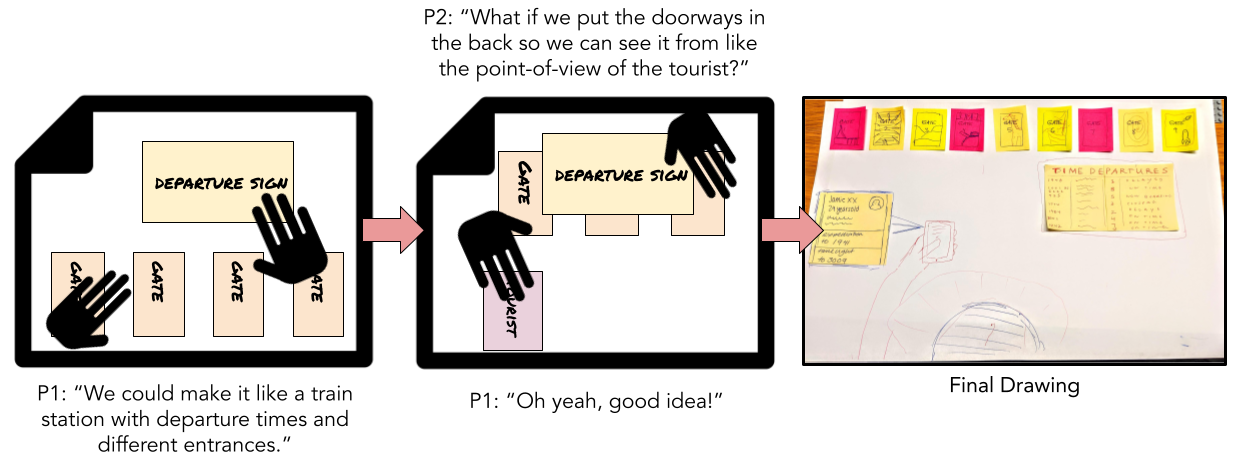
\includegraphics[width=\textwidth]{abstraction/figures/main_fig.png}
  \caption[A group from our study discussed composition and layout ideas for a collaborative sketch using abstract blocks.]{A group from our study discussed composition and layout ideas for a collaborative sketch using abstract blocks. These tangible and malleable blocks remove the need for smaller details and emphasize exploration. The prompt for the sketch was ``A scene with a time-travelling tourist.''}~\label{fig:blocks}
\end{figure}

% We hypothesize that this form of structured abstraction helps groups break down sketches into discrete, adaptable parts to communicate high-level ideas.
%---
%THINKING WiTH BOXES

An observational study investigated abstract blocks in a collaborative task. Six groups of novices ($n=19$) created drawings collaboratively. We audio and video recorded sessions and interviewed groups in a retrospective think-aloud. Groups used a paper implementation of abstraction blocks, using sticky notes, to plan a sketch based on a prompt. Working with simple blocks helped groups to see their drawings in terms of malleable, conceptual chunks. Tangible blocks helped groups discuss high-level concepts like `point-of-view` or `scale` and helped them quickly explore and change the composition of the drawing by editing the configuration of the blocks. Working at this more abstract, block level appeared to keep early discussion on more conceptual discussion rather than lower-level implementation details. These results suggest to us that offering (or even enforcing) abstract creation primitives like blocks catalyzes an emphasis on strategic and conceptual issues. 



\section{How is Abstraction Used in Creative Work?}

One definition of abstraction is that higher-level features are stable and static whereas lower-level features are those that can change in context \cite{shapira2012levels}. From an information storage perspective, high-level abstractions form units of information, or chunks, formed from recognized patterns \cite{Chase1973,Gobet2001,Gobet1998}. Early in creative work, higher-level abstractions enable the exploration of concepts rather than details such as when dancers use marking to think through an overall choreography \cite{kirsh2011marking} or when illustrators or designers use preliminary sketches to communicate rough thoughts \cite{Buxton2007, landay1996sketching, Tversky2011,Tversky2009}. Rubrics and templates are other forms of abstraction tools because they highlight structural goals that are adapted and refined through the addition of concrete details \cite{andrade2005teaching,yuan2016}. While experts utilize abstraction techniques like sketching to explore and engage in a reflective dialogue with others and their work \cite{schon1984reflective,Tversky1999,Tversky2009}, novices are often drawn to details \cite{jansson1991design,marsh1996examples,Smith1993}. Particularly in visual creative work, this may be because novices are hesitant of their drawing ability or perceive even sketching to be more permanent \cite{Hennessey,welch2000sketching}. This chapter presents abstraction blocks as a strategy for malleable, high-level chunking in visual creative work that eliminates the necessity for early-stage sketching. 

\subsection{Limited Support for Abstraction in Collaborative Creative Tools}
%TOOLS FOCUS ON DETAILS INSTEAD OF ABSTRACTION
Particularly for online collaboration in creative work, tools and strategies for abstraction are limited. Many online projects take a crowdsourcing workflow approach, breaking down larger projects into smaller microtasks with a global goal to ensure coherence even in asychronous collaborations \cite{Hahn2016}. For text-based projects such as writing a collaborative story, workflows that decompose the work into concrete chunks and allow for interdependent contributions can facilitate structured, high-quality work \cite{Kim2016,Kim2017,Retelny2014,Salehi2018,Valentine2017}. Visual creative work like drawing is similar to that of written work in that an overall theme and composition need to be developed to create a cohesive final artifact, but while text has inherent sequential structure, images are not linear and not as easily broken down into independent workable parts \cite{Johnson-Laird1983}. 

Communication of abstract ideas within these collaborations may rely more on coordinating actions and developing rapport \cite{Davis2017,Davis2016}, which can be difficult in online settings where groups must rely on technological affordances to effectively communicate \cite{Hollan1992,Jensen2018}. Strategies for abstraction in collaborative visual work are limited in implementation. For example, SwarmSketch \cite{swarm} allows users to influence the direction of a collaborative drawing by contributing a single ink stroke however they like, but does not provide tools for communication between contributors or structure for how work should be coordinated. As a result, many drawings become a haphazard collection of strokes that no longer match the original goal and are difficult to change \cite{Boxer2005}. The Johnny Cash Project \cite{TheJohnnyCashProject2012} also predefines the overall project goal of collaboratively making a hand-drawn music video and coordinates contributor work through individual tasks (such as tracing over a designated image); however, it necessarily limits contributions to a single level of detail for ease of coordination, preventing contributors from influencing the direction of the project as a whole. 

\begin{figure}
\centering
  %\vspace{-0.2in}
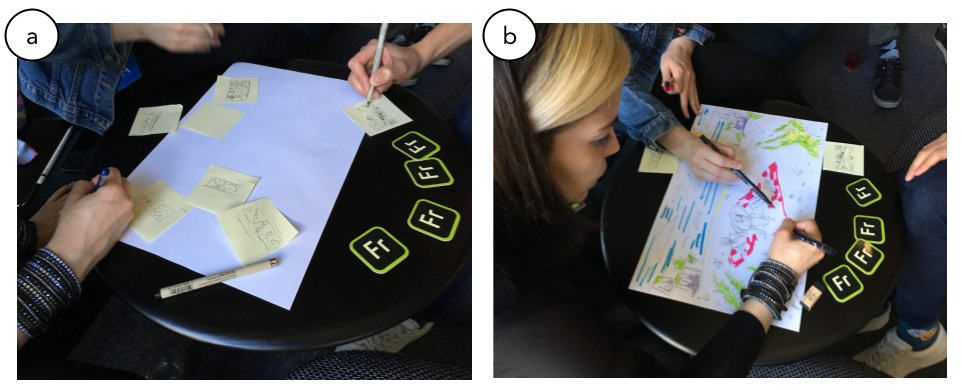
\includegraphics[width=\textwidth]{abstraction/figures/expert.png}
\vspace{-0.2in}
  \caption{a) Experts started planning by sketching multiple thumbnails that conveyed overall structure and composition more than details. b) These composition sketches provided a reference for experts during drawing.}
  ~\label{fig:expert}
  \vspace{-0.2in}
\end{figure}

``Blank page'' tools allow for open-ended abstraction, but are often unstructured. The problem with remaining too abstract or unstructured, especially in collaborative work, is that communication and consensus may get lost in the woods \cite{hinds1999curse,hinds2001}. Multiplayer experiences such as those in  Figma (www.figma.com), Google Docs \cite{wang2015students}, or collaborative drawing canvases (www.drawpile.net) enable a large range collaboration strategies, from allowing anyone to modify anything through pixel-perfect editing, to splitting the canvas or document into sections and assigning collaborators to each part. Digital whiteboards \cite{Ishii1992} and sketch interfaces \cite{lin2000denim} similarly give users the freedom to express their thoughts with as much or as little detail as desired. However, these systems leave it to the users to develop their own external collaboration structures. Without prerequisite knowledge of abstraction strategies, novices especially may continue to lean towards specific details, such as the exact specifications of a sketch \cite{welch2000sketching} or precise wording of an essay \cite{sommers1980revision}. Abstraction blocks ground the exploration and communication of abstract ideas to movable boxes to shift focus away from low-level details while giving tangible artifacts with which to interface.





\chapter{Abstraction Blocks: Thinking with Boxes for Flexible Abstraction \& Collaboration}
% \chapter{Thinking with Boxes: Tools for Abstraction Enable Flexible Creative Work}
\label{chapter:abstraction}
\begin{quote}
Effectively communicating ideas is an important part of creative collaboration, particularly in getting started and generating ideas. One major challenge of collaboration is the pull of concrete details over conceptual concerns as concrete details often stand out more than high-level structure. For example, discussing specific details of a drawing early can pull attention away from assessing whether the drawing's composition works as a whole. This chapter investigates using a strategy called \textit{abstraction blocks}, movable shapes to represent size and position of drawing elements without the need (or ability) to specify concrete details, for collaborative drawing. We hypothesized that structuring abstraction around these blocks enables more flexible exploration and communication. In an observational study of six synchronous small groups ($n=19$) sketching collaboratively, we found that abstraction blocks enabled more iterative and flexible exploration of drawing compositions. Groups using abstraction blocks explored alternative drawing compositions and discussed high-level concepts such as point-of-view and scale compared to sketching alone.
\end{quote}

\section{Introduction}
% Making Abstraction Concrete
We communicate with others at all stages of creative work, from ideation to critique \cite{mamykina2002collaborative}. 
For example, when writing, collaborators often first generate a high-level outline, later shifting focus to a lower level by revising grammar \cite{sommers1980revision}. Visual work like web design also spans abstraction levels, from task goals to deciding specific element placement \cite{klemmer2001designers}. Early on, high-level concerns should dominate. For example, in drawing, exploring various compositions early is more important than deciding what specific characters look like. Lightweight sketches serve as exploratory tools to visually communicate ideas in domains from architecture to illustration \cite{Buxton2007,Tversky2011,Tversky2009}. Dancers use marking to physically think through choreography without focusing on the details of the dance \cite{kirsh2011marking}. Designers use paper prototyping \cite{Snyder2003} and storyboarding \cite{landay1996sketching} to collaboratively think through a goal without focusing heavily on concrete details. These `blocking' strategies help people view work as high-level chunks rather than individual elements \cite{Chase1973,Gobet1998,chi1981categorization} While abstract chunking and high-level exploration are important for both ideation and collaboration, the emphasis of online collaboration in creative tasks has been on refinement and revision of completed work. Focusing on details early on can shift a group's attention to refinement rather than rough exploration, which can lead to fixation on a single idea \cite{jansson1991design,simon1972theories} or iterating incrementally on a previous idea rather than trying a potentially new and better concept \cite{Dow2009,Little2010,Yu2016}. 

We know that abstraction helps \emph{individuals} focus on high-level concerns \cite{Chase1973}; a combination of early stage abstraction and structure may also help \emph{collaborators} focus on high-level ideation and communicate with one another. We hypothesize that explicitly supporting `chunks' for early-stage design catalyzes collaborators' ability to revise at an appropriate level of abstraction by breaking down sketches into discrete, adaptable parts. Inspired by expert uses of chunking and tools that use tangible interfaces and techniques \cite{klemmer2001designers,Resnick2009}, this chapter investigates using abstract blocks as a form of visual chunking and a tool for structuring group communication. 
For example, a drawing of a tourist at a train station might consist of several abstract blocks to represent placement of these elements (Figure \ref{fig:blocks}); these blocks can be directly manipulated to communicate desired changes, suggestions, or ideas without the immediate need to change the sketch itself. Users can choose to label the blocks either through text or pictorially, giving flexibility in how they choose to represent their ideas. We focus on sketching as an initial exemplar domain of the broader class of creative work because sketching is an easily accessible medium that only requires pen and paper and is a beneficial tool for visual communication \cite{Buxton2007,Tversky1999}.

\begin{figure}
\centering
  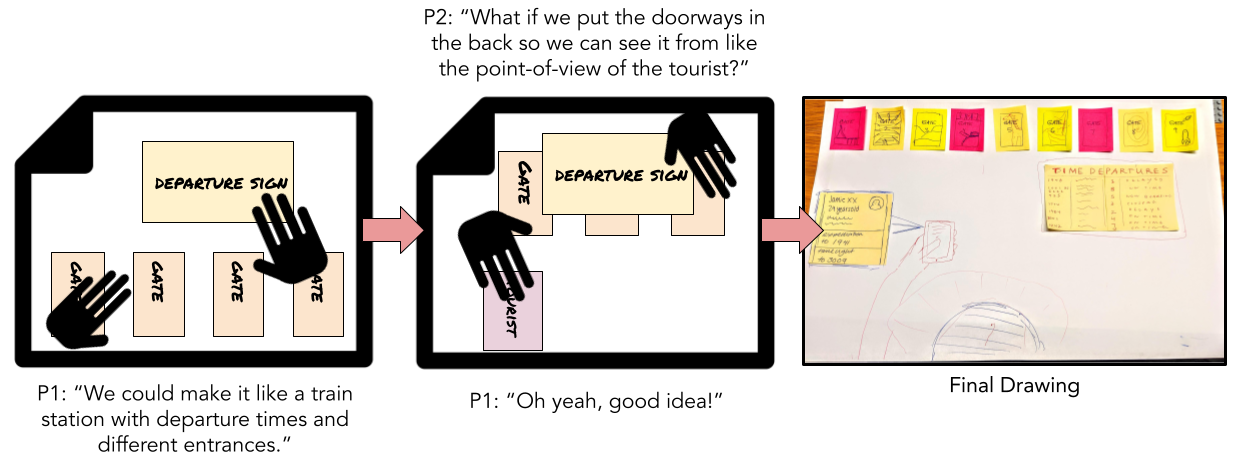
\includegraphics[width=\textwidth]{abstraction/figures/main_fig.png}
  \caption[A group from our study discussed composition and layout ideas for a collaborative sketch using abstract blocks.]{A group from our study discussed composition and layout ideas for a collaborative sketch using abstract blocks. These tangible and malleable blocks remove the need for smaller details and emphasize exploration. The prompt for the sketch was ``A scene with a time-travelling tourist.''}~\label{fig:blocks}
\end{figure}

% We hypothesize that this form of structured abstraction helps groups break down sketches into discrete, adaptable parts to communicate high-level ideas.
%---
%THINKING WiTH BOXES

An observational study investigated abstract blocks in a collaborative task. Six groups of novices ($n=19$) created drawings collaboratively. We audio and video recorded sessions and interviewed groups in a retrospective think-aloud. Groups used a paper implementation of abstraction blocks, using sticky notes, to plan a sketch based on a prompt. Working with simple blocks helped groups to see their drawings in terms of malleable, conceptual chunks. Tangible blocks helped groups discuss high-level concepts like `point-of-view` or `scale` and helped them quickly explore and change the composition of the drawing by editing the configuration of the blocks. Working at this more abstract, block level appeared to keep early discussion on more conceptual discussion rather than lower-level implementation details. These results suggest to us that offering (or even enforcing) abstract creation primitives like blocks catalyzes an emphasis on strategic and conceptual issues. 


\section{How is Abstraction Used in Creative Work?}

One definition of abstraction is that higher-level features are stable and static whereas lower-level features are those that can change in context \cite{shapira2012levels}. From an information storage perspective, high-level abstractions form units of information, or chunks, formed from recognized patterns \cite{Chase1973,Gobet2001,Gobet1998}. Early in creative work, higher-level abstractions enable the exploration of concepts rather than details such as when dancers use marking to think through an overall choreography \cite{kirsh2011marking} or when illustrators or designers use preliminary sketches to communicate rough thoughts \cite{Buxton2007, landay1996sketching, Tversky2011,Tversky2009}. Rubrics and templates are other forms of abstraction tools because they highlight structural goals that are adapted and refined through the addition of concrete details \cite{andrade2005teaching,yuan2016}. While experts utilize abstraction techniques like sketching to explore and engage in a reflective dialogue with others and their work \cite{schon1984reflective,Tversky1999,Tversky2009}, novices are often drawn to details \cite{jansson1991design,marsh1996examples,Smith1993}. Particularly in visual creative work, this may be because novices are hesitant of their drawing ability or perceive even sketching to be more permanent \cite{Hennessey,welch2000sketching}. This chapter presents abstraction blocks as a strategy for malleable, high-level chunking in visual creative work that eliminates the necessity for early-stage sketching. 

\subsection{Limited Support for Abstraction in Collaborative Creative Tools}
%TOOLS FOCUS ON DETAILS INSTEAD OF ABSTRACTION
Particularly for online collaboration in creative work, tools and strategies for abstraction are limited. Many online projects take a crowdsourcing workflow approach, breaking down larger projects into smaller microtasks with a global goal to ensure coherence even in asychronous collaborations \cite{Hahn2016}. For text-based projects such as writing a collaborative story, workflows that decompose the work into concrete chunks and allow for interdependent contributions can facilitate structured, high-quality work \cite{Kim2016,Kim2017,Retelny2014,Salehi2018,Valentine2017}. Visual creative work like drawing is similar to that of written work in that an overall theme and composition need to be developed to create a cohesive final artifact, but while text has inherent sequential structure, images are not linear and not as easily broken down into independent workable parts \cite{Johnson-Laird1983}. 

Communication of abstract ideas within these collaborations may rely more on coordinating actions and developing rapport \cite{Davis2017,Davis2016}, which can be difficult in online settings where groups must rely on technological affordances to effectively communicate \cite{Hollan1992,Jensen2018}. Strategies for abstraction in collaborative visual work are limited in implementation. For example, SwarmSketch \cite{swarm} allows users to influence the direction of a collaborative drawing by contributing a single ink stroke however they like, but does not provide tools for communication between contributors or structure for how work should be coordinated. As a result, many drawings become a haphazard collection of strokes that no longer match the original goal and are difficult to change \cite{Boxer2005}. The Johnny Cash Project \cite{TheJohnnyCashProject2012} also predefines the overall project goal of collaboratively making a hand-drawn music video and coordinates contributor work through individual tasks (such as tracing over a designated image); however, it necessarily limits contributions to a single level of detail for ease of coordination, preventing contributors from influencing the direction of the project as a whole. 

\begin{figure}
\centering
  %\vspace{-0.2in}
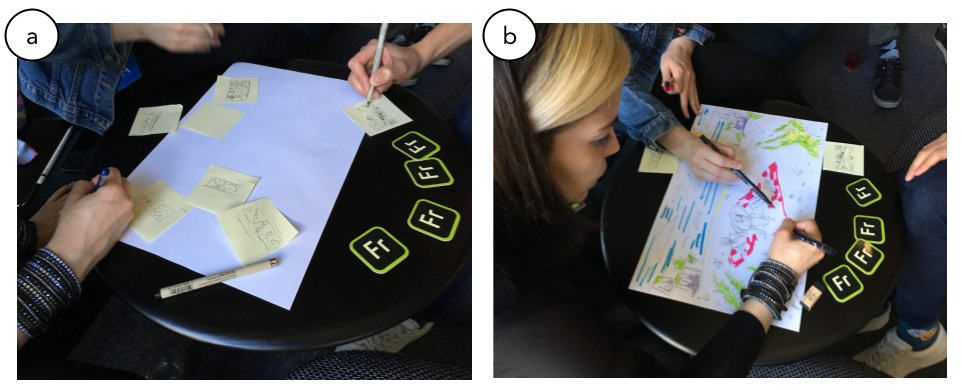
\includegraphics[width=\textwidth]{abstraction/figures/expert.png}
\vspace{-0.2in}
  \caption{a) Experts started planning by sketching multiple thumbnails that conveyed overall structure and composition more than details. b) These composition sketches provided a reference for experts during drawing.}
  ~\label{fig:expert}
  \vspace{-0.2in}
\end{figure}

``Blank page'' tools allow for open-ended abstraction, but are often unstructured. The problem with remaining too abstract or unstructured, especially in collaborative work, is that communication and consensus may get lost in the woods \cite{hinds1999curse,hinds2001}. Multiplayer experiences such as those in  Figma (www.figma.com), Google Docs \cite{wang2015students}, or collaborative drawing canvases (www.drawpile.net) enable a large range collaboration strategies, from allowing anyone to modify anything through pixel-perfect editing, to splitting the canvas or document into sections and assigning collaborators to each part. Digital whiteboards \cite{Ishii1992} and sketch interfaces \cite{lin2000denim} similarly give users the freedom to express their thoughts with as much or as little detail as desired. However, these systems leave it to the users to develop their own external collaboration structures. Without prerequisite knowledge of abstraction strategies, novices especially may continue to lean towards specific details, such as the exact specifications of a sketch \cite{welch2000sketching} or precise wording of an essay \cite{sommers1980revision}. Abstraction blocks ground the exploration and communication of abstract ideas to movable boxes to shift focus away from low-level details while giving tangible artifacts with which to interface.

\section{Abstraction Blocks: Thinking with Boxes}

\subsection{Formative Interviews: How Do Experts Collaborate?}
To investigate the role of abstraction in how experts communicate during collaboration, we observed three proficient illustrators recruited from a local drawing and illustration club perform a collaborative drawing task. In this task, the group made a single drawing together based on an open-ended prompt, ``Draw a scene of a place that makes you happy.'' We provided the group with paper, sticky notes, pencils, colored pens and markers, and a single large sheet of paper as the canvas for their drawing. We observed that experts used abstraction in three main ways.

First, experts used abstraction to quickly capture ideas from members of the group. In planning their drawing, the group first created several small thumbnail sketches on sticky notes as members generated ideas for various drawing compositions as part of their planning process (Figure \ref{fig:expert}). Creating small, abstract drawings is a common technique for visually generating ideas and solving problems \cite{poore1967composition,Poore1967}. In this collaborative context, this technique additionally functioned as a way to communicate and confirm thoughts between members of the group, throwing out various ``what if'' scenarios: \textit{``What if we made like ice cream dogs? I know that's silly, but it conveys happy.''} Sometimes a participant would sketch a thumbnail themselves and place it in the center to show the group their idea. Other times, a participant would draw a thumbnail sketch as a different participant was verbally describing their idea, while asking for confirmation that their sketch of the idea was accurate. In a post-interview, the experts mentioned that they learned the thumbnailing technique from their art education and practice.

\begin{figure}
\centering
  %\vspace{-0.2in}
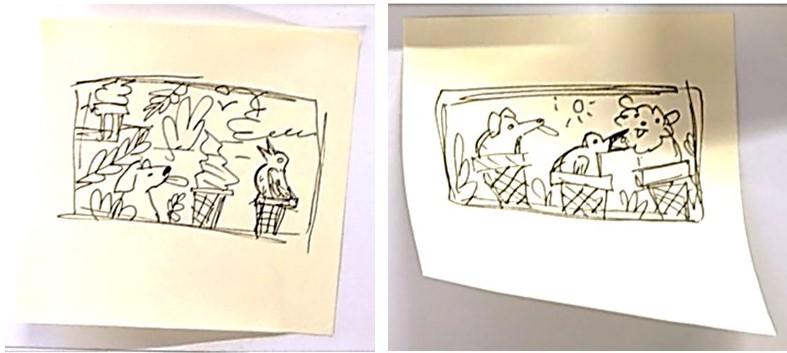
\includegraphics[width=\textwidth]{abstraction/figures/thumbnails.jpg}
\vspace{-0.2in}
  \caption{An expert participant sketched these two thumbnails to illustrate and explore alternate compositions for similar elements.}
  ~\label{fig:thumbnail}
  \vspace{-0.2in}
\end{figure}

Second, experts used abstraction to reduce unnecessary work by reusing elements that had already been drawn. For example, Figure \ref{fig:thumbnail} shows two thumbnail sketches that contain similar elements in different layouts and compositions. To choose a direction for their sketch, the group placed the thumbnail sketches in front of them and discussed to come to a consensus. These sketches conveyed relative positioning of sketch elements rather than specific details of the drawing. The group decided on an overall composition while adding in ideas contributed through other group members' thumbnails.

Lastly, experts used abstraction as a way to anchor discussions about how to proceed.
After deciding on an overall composition, the expert group  assigned work to each of its members. However, rather than assigning work based on areas of the canvas paper, the group delegated work based on the elements in the composition they had developed together: ``\textit{You draw the background since it's your design, you draw the foliage, and I'll draw the [character]?}'' This gave a clear sense in who would draw which part of the sketch and drew from their rough composition plan. 

% \begin{figure}
% \centering
%   %\vspace{-0.2in}
% 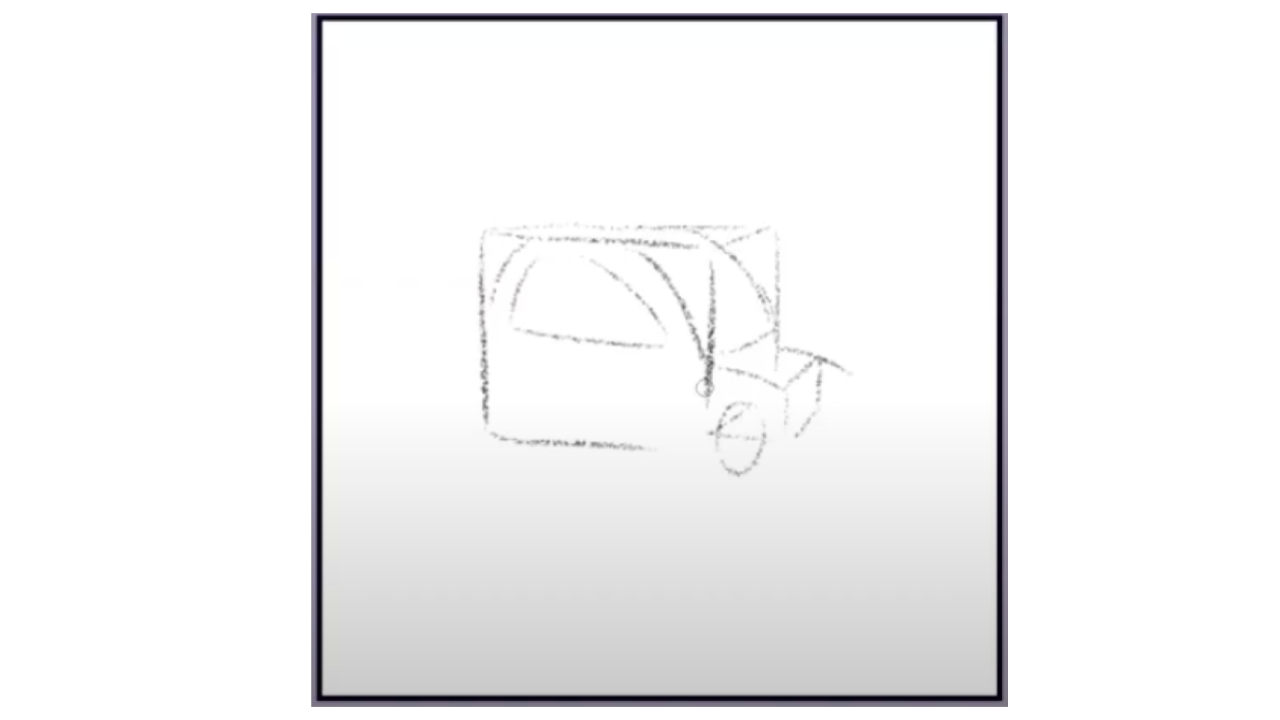
\includegraphics[width=.8\textwidth]{abstraction/figures/expertbox.png}
% \vspace{-0.2in}
%   \caption{An expert demonstrating how box shapes can be used as the basis for drawing nearly any object.}
%   ~\label{fig:expertbox}
%   \vspace{-0.2in}
% \end{figure}

After completing their rough sketch, the experts began adding details. This part of drawing process was much more improvisational; for example, individual members of the group freely colored in areas of the sketch with little or no coordination with other members of the group. In a post-interview, experts noted that the drawing phases did not require as much communication or coordination, since much of the sketch had been previously outlined, reflecting the key concepts of loosely coupled work and maintaining common ground \cite{olson2000distance}.

\subsection{Abstraction Blocks: Making the Abstract Concrete}
From prior work on expert abstraction strategies and our observations of the expert illustrators, we distill these strategies into \textit{abstraction blocks}. We implement these blocks using paper sticky notes as representations of blocking, or chunking, elements that can be shaped, edited, and moved around as desired (Figure \ref{fig:blocks}). We chose to characterize abstraction as abstraction blocks because we expected it would be easy for novices to understand and because it mimics common abstraction strategies used by experts in our chosen domain of drawing \cite{poore1967composition}. While sketches are an abstract representation themselves, novices especially still focus on details rather than exploratory goals during sketching \cite{welch2000sketching}. Encouraging participants to use blocks allows participants to convey rough composition without the need for sketching, emphasizes the spatial relationships between components of a drawing rather than its details, and express a creative vision without worrying about drawing skill or matching the aesthetic style of other collaborators.


\section{Observational Design Study}
\label{sec:abs_study}
In this observational design study, we wanted to observe how groups of people with varying levels of expertise in art would work together on a drawing task, and see how collaboration would be affected by usage of abstraction strategies. While the experts we observed used abstract composition sketches to create the ``undersketch'' of their eventual drawing, we anticipated that most of our participants would not know how to do this. 

\subsection{Method}

\subsubsection{Participants}
Six groups of two to four people ($n=$ 19, 11 female, average age $=$ 28 years) participated in a collaborative drawing task. Participants were recruited from a technology company and local art school through an email advertisement and signed up for scheduled time slots. Though group members were not required to know each other, at least two people from each group had an existing working relationship. The average self-reported drawing experience level was 1.95 ($SD=$ 0.78) out of 4, with 1 being no experience and 4 being expert level. We randomly assigned groups to two conditions: three to \textit{abstraction} and three to \textit{freeform}. Each condition comprised one group of size two, one group of three, and one group of four to explore how communication potentially changes as function of group size. While most groups were co-located, one group in each condition consisted of distributed participants using an online shared canvas (Google Jamboard) and video conferencing (BlueJeans). Observing these distributed groups gave insight on the impact of abstraction on co-located versus remote collaboration. Participants received a \$25 USD gift card for their time. All sessions were video and audio recorded with the experimenter taking note of critical moments during each session.  

\subsubsection{Procedure}
For \textit{abstraction} groups, we first presented a short tutorial of how to use abstraction blocks (Figure \ref{fig:blocks}). Our tutorial explained that participants could use the blocks to represent where a sketch element would be in a drawing. They were free to use text, sketches, or the blocks as they pleased. Groups each made a collective drawing in response to the prompt, ``A scene with a time-traveling tourist.'' We chose a fictional storytelling prompt and drawing task because it does not require any domain knowledge and enables collaborative ideation and interaction \cite{Davis2017}. The task was 20 minutes long and broken into three segments to control for time spent in each part of the process across conditions: five minutes for brainstorming, five minutes for planning and drafting, and ten minutes for drawing. Groups could use paper, pens, pencils, and colored pencils throughout the task. We asked each group to deliver their drawing on one sheet of paper by the end of the study session.

During brainstorming, participants discussed ideas without worrying about drawing yet. Before the planning phase, we gave a short explanation of basic composition concepts and instructed groups to focus on drawing composition during planning. \textit{Abstraction} groups were given standard size and small sticky notes to use and presented with the blocking strategy at this time. Google Jamboard's sticky note feature and pen tools simulated using physical sticky notes and regular analog sketching in the remote sessions. \textit{Freeform} groups were able to plan their drawing in any manner. Following planning, groups collaboratively worked on their drawing for the remainder of the task. Directly after the drawing task, the experimenter replayed recorded critical moments on a computer screen for groups (and through the sharescreen feature for digital groups), asked them to reflect on these clips, and reviewed any additional moments mentioned during the discussion. 

\subsection{Results}
To find emergent themes of how groups interacted with drawing artifacts and each other, we noted interesting behaviors and critical moments in each of the sessions, looking for commonalities across groups and between conditions. We found that groups that used abstraction blocks engaged in more conceptual discussion and worked together in a more flexible manner.

\subsubsection{Abstraction Enabled Integrated Collaboration} 
Compared to freeform sketching, abstraction blocks seemed to help groups form a strong shared understanding of each others' ideas. To represent drawing elements, \textit{abstraction} groups placed sticky notes on their draft paper to create a blueprint of their composition. For example, Group 2 (\textit{abstraction}) put three sticky notes together to represent a focal point (a train) of their drawing while using the smaller sticky notes to represent smaller elements (individual people). These sticky notes were labeled with a brief written description or a small sketch showing what the block was supposed to represent.

\begin{figure*}
\centering
  \vspace{-0.2in}
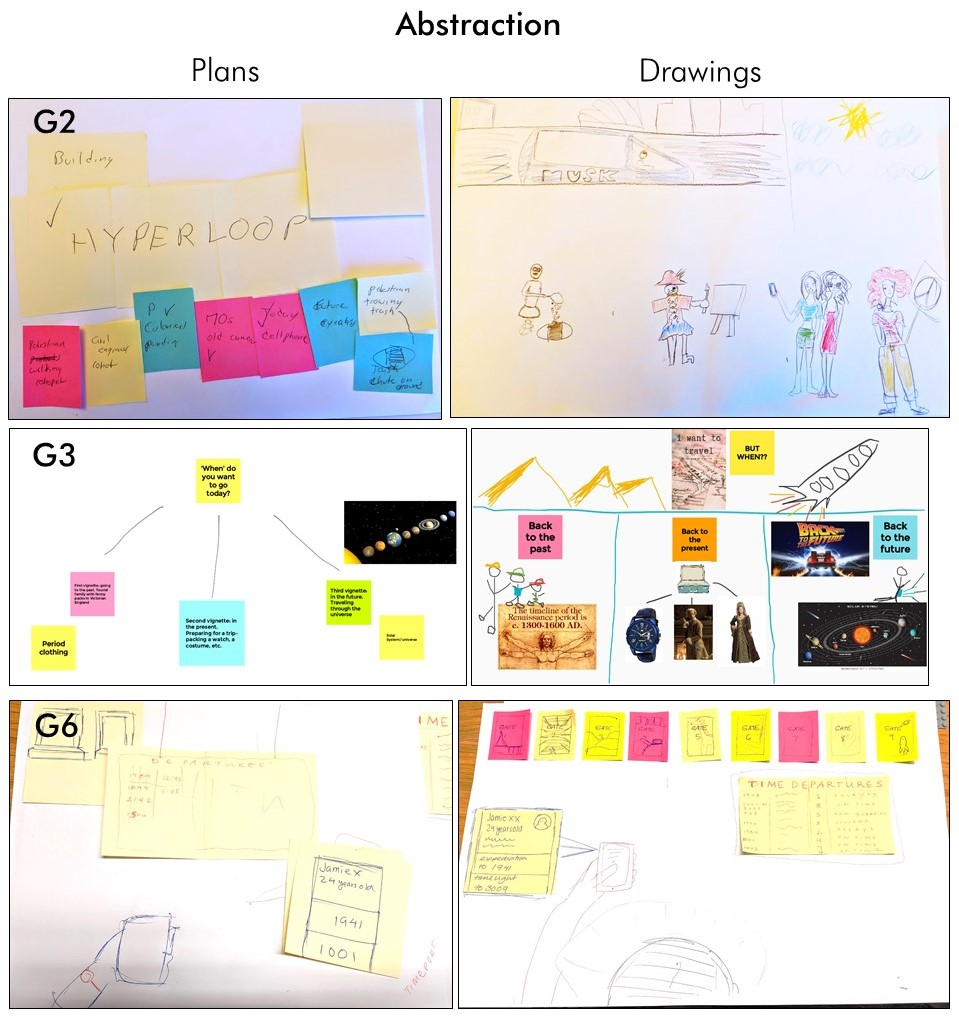
\includegraphics[width=\textwidth]{abstraction/figures/abs.jpg}
% 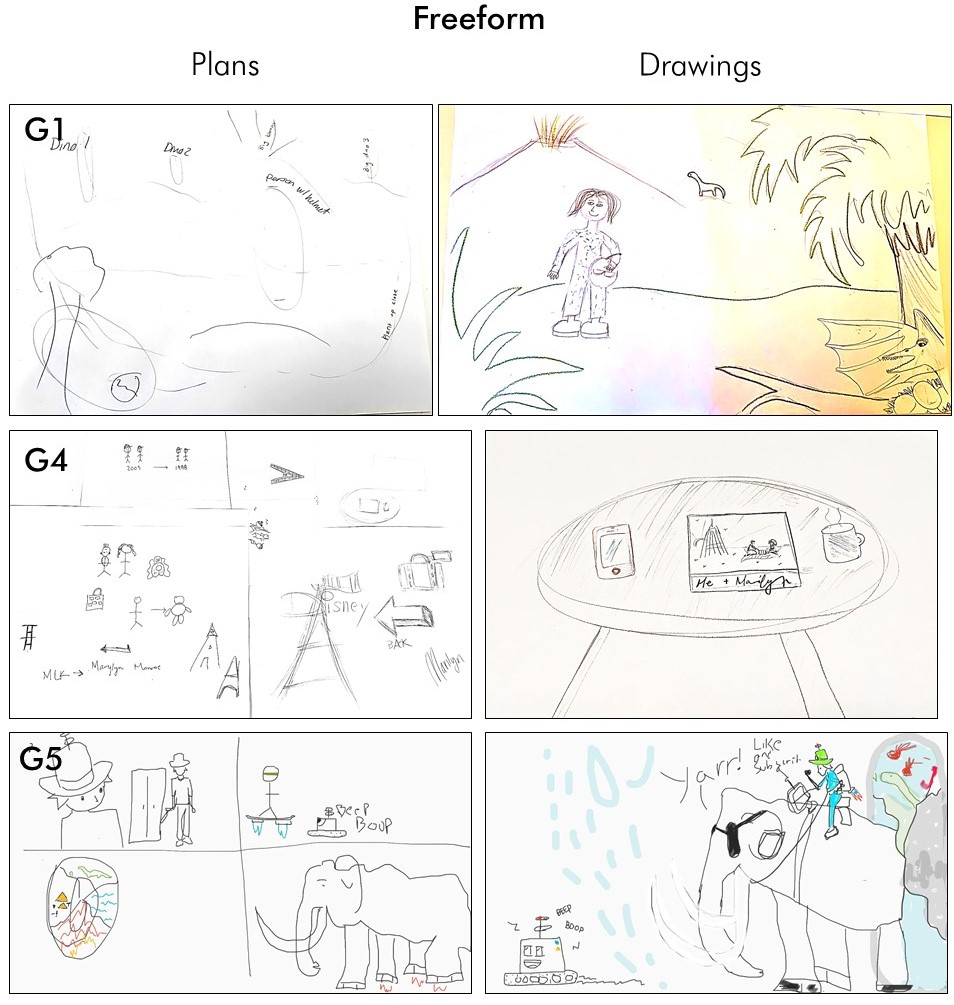
\includegraphics[width=\textwidth]{abstraction/figures/freeform.jpg}
\vspace{-0.3in}
  \caption{\textit{Abstraction} groups developed composition plans from the abstract blocks that formed the basis of their final drawings.}
  ~\label{fig:abs_drawings}
  \vspace{-0.2in}
\end{figure*}

\begin{figure*}
\centering
  \vspace{-0.2in}
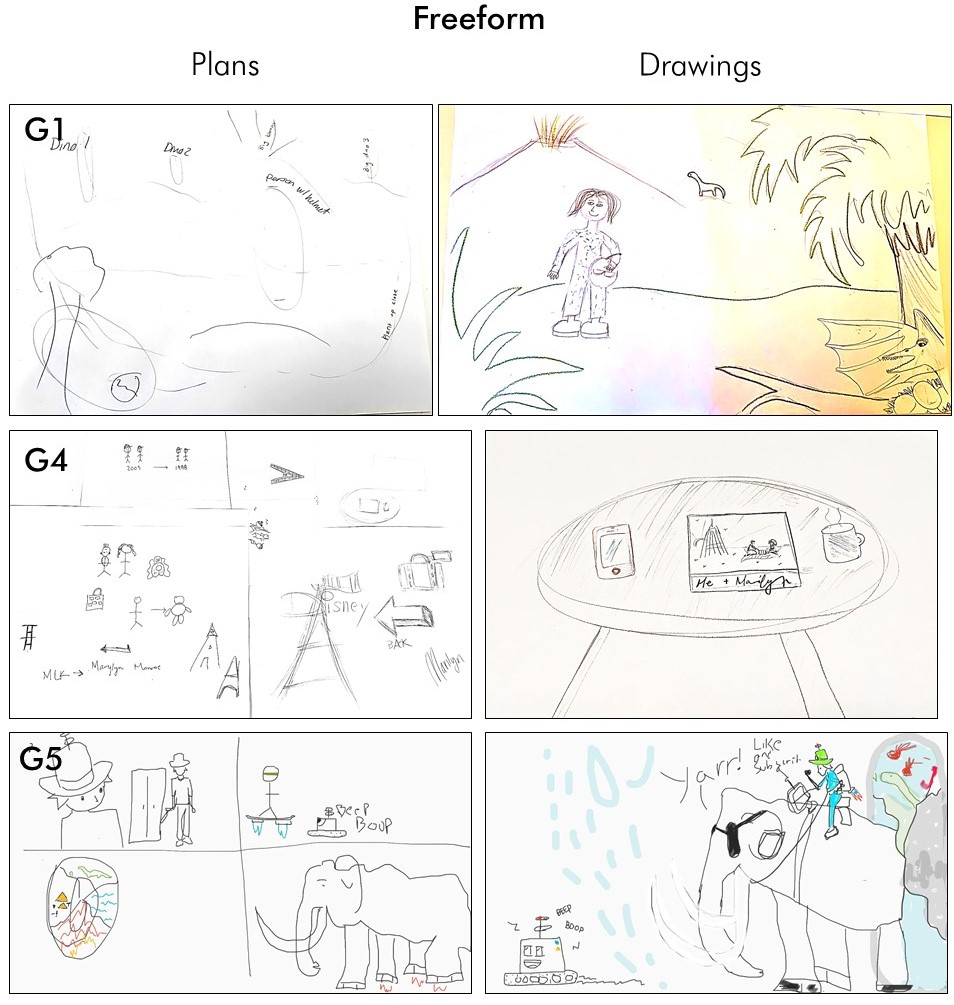
\includegraphics[width=\textwidth]{abstraction/figures/freeform.jpg}
\vspace{-0.3in}
  \caption{\textit{Freeform} groups tended to sketch individual details before deciding on a final composition.}
  ~\label{fig:freeform_drawings}
  \vspace{-0.2in}
\end{figure*}

Similar to the thumbnail sketches created by the experts we observed, abstraction blocks helped anchor discussion by providing shared representations of what members of the group were thinking about: \textit{``I think once someone gave us a visual view of what [they were] thinking, I feel like we all were like ‘Yeah! Perfect'.''} (P5, \textit{abstraction}). P6 (\textit{abstraction}) similarly said in the post-interview that \textit{``everyone has different ways of placing things on paper so once we laid out that this goes here, I think it was helpful for all of us to just visualize the layout of all the things we were talking about.''}

In contrast, Group 1 was the only \textit{freeform} group to make a lightly sketched blueprint of their drawing due to one participant's prior domain knowledge in photography and compositions. 

In other \textit{freeform} groups, participants sketched their own individual drawing elements on separate sheets of paper or divided up their shared drawing sheet into areas ``owned'' by each member of the group (Figure \ref{fig:freeform_drawings}). For example, Group 4 members each sketched their own version of the Eiffel Tower on their scratch paper. 
For \textit{freeform} groups, planning seemed to be oriented around making decisions about specific details of the drawing rather than explore options for the drawing's overall composition.

These differences in how groups approached planning their drawing also affected how they allotted drawing work among individuals. \textit{Abstraction} groups tended to use the blocks they had created as a way to define who should draw what. For example, Group 2 (\textit{abstraction}) assigned each person to draw one of the block elements on their composition plan. They physically checked off the blocks on their plan as they were drawing to mark which ones they completed:

\begin{quote}
    P3: \textit{``I can take `colonial' [people].''}\\ 
    P5: \textit{``We'll take the `today' people on this side.''}\\
    --- Group 2 (\textit{abstraction})
\end{quote}

\textit{Freeform} groups focused instead on smaller, individual elements and focused on the details of these elements. For example, Group 1 (\textit{freeform}) split up their work by individual characters: \textit{``So do you want to start drafting the person and play around with outfits, and I'll do the dinosaurs?''} (P1, \textit{freeform}). However, because \textit{freeform} participants had individually planned portions of the drawing separately from others in their group, they encountered conflicts in their understanding of the drawing's composition as sketching progressed.

One \textit{freeform} participant in Group 5 asked another group member to redraw and switch the orientation of another element during drawing: \textit{``Can you draw the portal on the right because I drew the mammoth from right to left, and this will be very complicated for me to draw it from left to right.''} (P16 \textit{freeform}). There was also sometimes confusion about what each person should work on during drawing. In the post-interview, P13 (\textit{freeform}) said, \textit{``I didn't quite know what I was doing, everyone seem to have their own parts...and I was like 'what should I do?'''}. P14 (\textit{freeform}) also mentioned that he wished his group had done more concrete outlining beforehand so \textit{``people can work more independently instead of having to wait for another part to be done.''} 

\subsubsection{Abstraction Groups Focused on High-Level Decisions}
Groups that used abstract blocks seemed to discuss higher-level concepts like general theme and layouts throughout the drawing process. For example, when talking about how to depict a person looking at a time travel app on his phone, Group 6 (\textit{abstraction}) included light sketches on their blocks (Figure \ref{fig:abs_drawings}) to capture and discuss concepts like point of view, background focus, and scale during planning:

\begin{quote}
    P19: \textit{``Maybe we're still in his point of view, like he's looking at his phone.''}\\
    P17: \textit{``The scale can be small because we probably don't want to get too detailed, but the idea is just to convey that it's a travel app.''}\\
    P18: \textit{``And maybe we can have a thing where it's like zoomed in to show this is what he's holding.''}\\
    --- Group 6 (\textit{abstraction})
\end{quote}

Group 3 (\textit{abstraction}), the digital group, spent their planning time setting high-level goals for their drawing. They made blocks with questions for what they wanted to achieve in their drawing rather than making individual sketches: \textit{``Do you wanna have the main question on the top, and then like three vignettes below?''} (P8, \textit{abstraction})

\begin{figure}[b!]
\centering
  \vspace{-0.25in}
  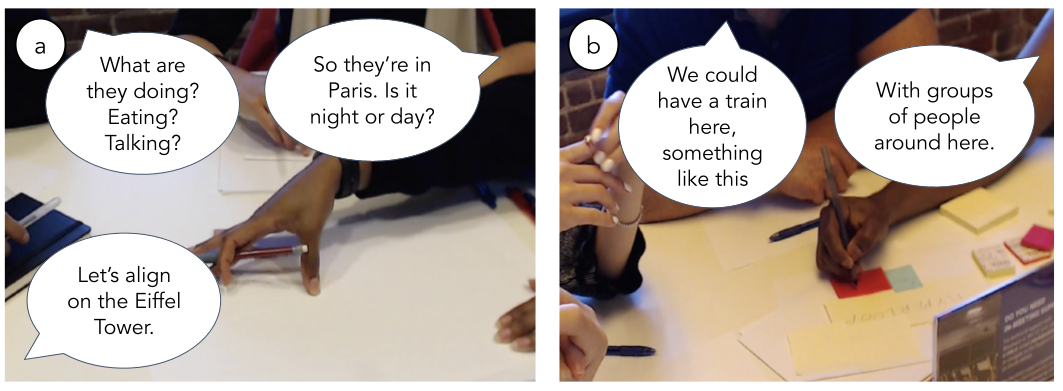
\includegraphics[width=.9\columnwidth]{abstraction/figures/planning.png}
  \caption{(a) \textit{Freeform} groups discussed details early without making concrete sketches until their final drawing. (b) \textit{Abstraction} groups instead used abstract blocks to concretely discuss and sketch a drawing composition.}~\label{fig:tangible}
  \vspace{-0.2in}
\end{figure}

\textit{Freeform} groups instead had a tendency to discuss lower-level details during planning, corroborating findings from prior work \cite{jansson1991design, Little2010, Yu2016}. In Group 5 (\textit{freeform}), participants discussed incremental details for how specific elements should look. For example, when discussing how to show a time traveller coming out of a time travel portal:

\begin{quote}
    P15: \textit{``We could have different futures in the portal, like maybe one where the world is flooded.''}\\
    P14: \textit{``Looks like [P15] has gone in pretty hard on [drawing] the portal...so [P13] should draw the traveler.''}\\
    P15: \textit{``And then [P14] will add lasers to it.''}\\
    P14: \textit{``Yeah like laser accessories.''}\\
    --- Group 5 (\textit{freeform})
\end{quote}

Discussions would often chain together incrementally, adding more details to existing ideas rather than offering new directions to explore. For example, Group 4 (\textit{freeform}) similarly attended to details and discussed the specifics of what their subjects would be doing in their drawing despite being in the planning stage of the study session:

\begin{quote}
    P12: \textit{``What are they doing? Talking?''}\\
    P9: \textit{``Eating?''}\\
    P11: \textit{``Yeah, wine. Eating.''}\\
    P12: \textit{``Coffee?''}\\
    P11: \textit{``No, wine.''}\\
    P9: \textit{``Cheese?''}\\
    P11: \textit{``Yup, cheese. Macarons? Done.''}\\
    --- G4 (\textit{freeform})
\end{quote}

In contrast to the expert group we observed, where improvisational discussion of details occurred during the final stages of drawing, \textit{freeform} groups discussed these details during the early stages of ideation despite being encouraged to plan. For \textit{abstraction} groups, structuring abstraction around blocks oriented discussion around the overall composition of their drawing rather than the specific details of how the drawing should eventually look.

\subsubsection{Abstraction Enabled Flexible Workflows}
Abstraction blocks enabled \textit{abstraction} groups to easily explore alternative layouts and ideas.
\textit{Abstraction} groups described drawings as iterative and malleable, using their planning process to ask new ``what if'' scenarios. For example, while discussing how to draw a train station for time traveling, Group 6 (\textit{abstraction}) moved blocks to reflect their changing concept and even incorporated the blocks in their final drawing so they could continue to iterate and adapt (Figure \ref{fig:abs_drawings}):

\begin{quote}
    P17: \textit{``What if it's like multiple doors to multiple time periods?''}\\
    P19: \textit{``Oh and like this [sticky note] can be like the screen that shows all the departures.''}\\
    P18: \textit{``What if it was like this?''} (Takes a sticky note and moves it to another part of the planning canvas)\\
    --- Group 6 (\textit{abstraction})
    
\end{quote} 

Abstraction blocks were useful for planning, but also for making changes during drawing. For instance, during drawing Group six originally drew a screen in the middle of their page, but because they drew the screen on a block, they moved it further to the right side of the page. When asked their reasoning behind this change, P19 (\textit{abstraction}) said, \textit{``There was a moment [when] we realized that we didn't have enough space so that was a moment where we switched things around''}. Abstraction blocks helped in easily adapting their drawing plan even in the later stages of drawing. 

P17 (\textit{abstraction}) said the blocks felt impermanent: \textit{``When you draw something, it's permanent, but you can move [blocks] around, so you're not really committed.''}. P7 (\textit{abstraction}) also said direct manipulation of blocks helped in getting started: \textit{``Being able to take a sticky note and drag it to where you want it to go, it's so much easier to get started.''} (Figure \ref{fig:tangible}). Some participants thought the abstract blocks resembled other low-fidelity prototyping methods in helping groups view the drawing as piecemeal rather than a fixed whole. In particular, tangible pieces provided structure in building drawing plans: \textit{``It's about being tangible versus intangible so when we see [a block], we grasp onto the idea of that being something''} P18 (\textit{abstraction}). The flexibility in creating malleable chunks framed the drawing as impermanent, helping groups easily explore different ideas and concepts even during the final drawing phase. 

P7 (\textit{abstraction}) also said the abstraction blocks helped in getting started on the drawing: \textit{``it helped in [overcoming] that sort of blank page...and you're so daunted that you don't know how to get started...Then when you have a plan you can just get going on the drawing. There wasn't much discussion about what to do in the final stage because it had already been planned out.''} (P7, \textit{abstraction}).

In contrast, \textit{freeform} groups worked linearly and were often more hesitant to commit to and revise ideas. 
Sketching, even at a draft stage, was viewed as representing a permanent decision. In the post-interview, P12 (\textit{freeform}) mentioned expressing many ideas verbally, but being hesitant to start their drawing: \textit{``Nothing was concrete on the paper. So it was like we're just spitballing, but once you actually put ink to paper then it's like oh now we need to actually do it.''} Group 4 (\textit{freeform}) iterated on specific drawing elements individually (Figure \ref{fig:freeform_drawings}) because sketches on a shared sheet felt more permanent and committal. They aimed to form verbal consensus rather than exploring ideas the way \textit{abstract} groups did (Figure \ref{fig:tangible}). Here they discuss drawing a picture showing the time traveller posing with a historical figure:

\begin{quote}
    P9: \textit{``Do we want to fill the whole page or do we want to do a frame?''}\\
    P11: \textit{``Ooh let's frame it.''}\\
    P9: \textit{``So we agreed on a picture, yes?''}\\
    P10: \textit{``A picture within a picture? So is this like a postcard?''}\\
    P9: \textit{``So someone is like holding the postcard-''}\\
    P12: \textit{``Hands. Yes. I like that.''}\\
    --- Group 4 (\textit{freeform})
\end{quote}

Despite the fact that sketching is often useful as an abstraction tool \cite{Buxton2007,Tversky2009}, \textit{freeform} participants in our study still viewed sketching as costly and permanent, akin to final drawing. By providing \textit{abstraction} participants with a way to move their work around, abstract blocks instead made sketching together a more flexible and less daunting process.


\section{Discussion \& Future Work}
We investigated how directly manipulable abstract blocks affect communication in collaborative sketching. In an observational design study, we found that abstract blocks gave groups a way to break down drawing compositions through movable, simple shapes that de-emphasized details and permanence. They allowed \textit{abstraction} groups to communicate higher-level concepts and explore different ideas and compositions relative to \textit{freeform} groups, which used planning phases to discuss more superficial details rather than compositional concepts. In this section, we discuss the implications of these findings for future creativity support tools.

\subsection{Tools for Supporting Abstract Blocking}
This chapter investigated how scaffolding abstraction through abstract blocks affects exploration and communication in the task of collaborative drawing. 
In any collaborative task, communication can leave ephemeral, intangible artifacts that aid groups in coordinating actions and developing rapport \cite{Davis2017,Davis2016}. For example, group dynamic and physical gestures are important for ideation and building consensus in collaborative drawing tasks \cite{Bly1988, Tang1991}. In our observations, groups used both verbal and non-verbal forms of communication (like gesturing) to make decisions and share ideas \cite{goldin1999}. However, for \textit{abstraction} groups, abstract blocks helped participants concretely express intangible ideas through the placement of directly manipulable shapes, giving groups a malleable visualization of a concept that groups could modify as they conversed. The tangibility of making abstract concepts feel more concrete and importantly, changeable, seemed to be the primary benefit of abstraction blocks.

Groups could, of course, use blocking and similar abstraction strategies without a need for physical blocking tools. However, we observed in our study that \textit{freeform} groups did not use such strategies with the exception of one group who had prior experience in composition concepts through photography. Though sketches are meant to be blocking tools themselves, novices especially do not often separate exploratory sketching from refined drawing \cite{welch2000sketching}, as we observed in \textit{freeform} groups. When a concrete abstraction tool---abstract blocks---was made available, \textit{abstraction} groups were more inclined to create abstract representations. Some groups chose to use text to label blocks, others chose to lightly sketch, but importantly, \textit{abstraction} groups did not decorate blocks with heavy detail. Abstract blocks may have helped form common understanding of the drawing among collaborators \cite{olson2000distance}, helping groups maintain discourse on higher-level concepts.

Abstraction through abstract blocks may be even more beneficial in online settings where intangible communication is difficult. In such settings, groups must rely on technological affordances to effectively collaborate \cite{Hollan1992,Jensen2018}. 
Future collaborative tools could explicitly encourage abstract blocking, as opposed to requiring creators to figure out how to create abstract representations of their work themselves through existing tools (\textit{e.g.}, shape tools in Microsoft PowerPoint or Adobe Photoshop). 
One might also imagine creativity support tools where abstraction-oriented tools and detail-oriented tools can be used in a complementary manner. Our study also showed that there is a time and place for both kinds of representations in a collaborative creative task, and that there is value in being able to move between abstract and concrete representations of a drawing. Rather than needing two separate creativity tools---one for drafting a prototype and one for generating a final creative work---future work might investigate how a tool could help a group seamlessly navigate between two views of the same work.

\subsection{Supporting Creative Collaboration}
Our studies were done at a relatively small scale; abstract blocks could also support structured, large-scale crowdsourcing workflows. One way people seek to collaborate with a crowd in creative work is through asking for feedback or guidance online through discussion forums or creative communities \cite{kuznetsov2010rise,settles2013,wasko2005should} like Behance (www.behance.com). Much of the exchange and communication occurs via text comment feedback and relies on the creator to interpret suggestions, make changes, and update their work. Methods for structuring communication and exchange among crowd collaborators include assessment \cite{Dow2012} and framing \cite{hicks2016framing} prompts, but much of creative work relies on being to \textit{see} and understand changes. In our observations, we saw that collaborators formed a consensus around sketch ideas through abstract blocking. Similar to bringing in examples as a way to show ``something like this'' \cite{kang2018paragon}, abstract blocks enable quick ways to visually demonstrate ideas without focusing on details.

We also observed that groups used abstract blocks as a way to delegate tasks among collaborators, using the blocks as structured components for each collaborator. At a larger scale, abstract blocking could aid in managing input from a large number of contributors. For example, in leader-facilitated crowdsourcing approaches such as flash teams, a leader could assign modular tasks to a team through blocks \cite{Retelny2014,Salehi2018,Valentine2017} or signal which parts of a creative work are open for collaboration \cite{kim2014ensemble}. In remixing communities, contributors might use blocking to build upon certain structural components of an existing project \cite{Resnick2009}. From a social perspective, abstract blocks can also give a tangible way for interactively exploring ideas, which could be particularly useful in creative livestreams where a crowd can engage with an artist and contribute ideas beyond text chat suggestions and audience voting games \cite{Fraser2019}. Future work should examine how abstract blocking might impact communication at a larger-scale across domains.

\subsection{Rich Abstraction or Simple Details?}
One limitation of using abstract blocks was a decrease in improvisation. Serendipitous creativity can occur through collaborators building and improvising off others' ideas \cite{Davis2017,Davis2016}. We saw this in the \textit{freeform} groups where groups would chain ideas together, adding on different details as the group discussed. Because \textit{abstraction} groups created a concrete composition plan ahead of drawing, we observed more expedient drawing, but with less improvisation overall. However, we did observe improvisation and exploration during the planning process when groups were first discussing sketch ideas. \textit{Abstraction} groups explored alternative composition ideas rather than details early on, reflecting the expert process we observed. One area for future work is examining what level of abstraction is appropriate at different stages of creative work. Could abstraction blocks be used to also specify concrete details? This could allow both for exploration of high-level compositions as well as exploration of lower-level details while removing the need for higher-fidelity sketching. Tools could provide different modes for different levels of abstraction, similar to multi-layered interfaces that adaptively disclose functionality as the user progresses \cite{shneiderman2002promoting}.

Another limitation to using abstract blocks is it is unclear \textit{how much} detail should be abstracted. Some groups in our study simply used text labels on blocks to communicate an idea. Others used lightly sketched images. One group used image search to provide a reference for their idea. Each of these representations might differentially impact communication and understanding of the ideas presented. In addition, most \textit{abstraction} groups did not discuss nuanced composition details such as the direction a character is facing or their position in the drawing. Instead, much of the discussion emphasized placement since the abstract blocks focused on adjusting the sketch's overall layout. We saw more of a discussion of these details in the \textit{freeform} group. 

Our observational design study presents several opportunities for how tools might implement abstraction strategies such as abstract blocking. The first is in supporting large-scale collaboration. We observed how tangible and malleable blocks helped groups communicate and iterate upon abstract, exploratory ideas. One question for future research is how abstract blocks might support communicating composition details while maintaining flexibility and high-level focus without compromising the benefits afforded by removing detail in the first place. Another opportunity is in comparing the use of abstraction blocks in individuals versus a group and seeing how exploration strategies might change based on the level of communication and collaboration. Lastly, we examined abstraction blocks in sketching, but the concept could apply to any domain where high-level goals can be broken into chunks. Future work should examine the nature of abstraction and how abstraction blocks might be utilized in domains outside of visual work.

\subsubsection{Summary}
In this chapter, we describe and evaluate using abstraction blocks, a technique where visual content is \emph{abstracted} to simple shapes to facilitate communication and collaboration on visual creative work such as drawings. By abstracting elements of visual work, we found in an observational design study that people are more likely to explore high-level concepts such as composition and perspective and are less likely to fixate on details of an early idea. Collaborative tasks rely on effective communication between contributors. For novices especially, communicating higher-level goals and changes can be challenging without domain or procedural knowledge. Abstraction blocks scaffold this communication, using simple shapes as a flexible medium to create conceptual chunks rather than detailed sketches. This abstraction makes the invisible visible and the intangible tangible. Collaborative creativity support systems, both for visual creative work and beyond, should include mechanisms for attuning users to the right level of abstraction to explore and communicate higher-level concepts.

\subsubsection{Acknowledgements}
We thank our research participants for their time and efforts. This research was funded in part by Adobe Research.

This chapter, in part, is being prepared for submission for publication by Tricia J. Ngoon, Joy O. Kim, and Scott Klemmer. The dissertation author was the primary investigator and author of this material.

\chapter{Sh\"{o}wn: Adaptive Conceptual Guidance Aids Example Use}
\label{chapter:shown}
\begin{quote}
    Examples are powerful tools for creativity and can provide inspiration and structure. However, novices often don't know when to seek examples or how to apply them. 
    Showing real-time examples targeted to the current task (adaptive conceptual guidance) may help novices consider inspiration more often and better implement the ideas that examples illustrate.
    We explore this in a Wizard-of-Oz system, \textit{Sh{\"o}wn}, that presents examples based on the user's current activity while drawing a comic strip. \textit{Sh{\"o}wn}'s design is informed by interviews with novice and expert comic artists (n=18). A between-subjects experiment (n=24) found that adaptive conceptual guidance improved the clarity and uniqueness of drawings and stories compared to non-adaptive examples. Users also found the examples more useful and inspirational than those without adaptive guidance. Our results present an initial exploration of the challenges and benefits of contextually showing examples in interactive creativity tools.
\end{quote}
\section{Harnessing the Power of Examples in Creative Work}

A perennial challenge for novices is figuring out how to get started on a creative endeavor. Viewing and adapting others' work can help novices find traction in a mountain of possibility. Good examples can give inspiration, unveil new ideas, and highlight the advantages of alternative paths \cite{chan2011benefits,Siangliulue}. Examples can also help people compare and contrast different ideas across examples, drawing attention to important features (such as the composition or color scheme used by a painting) that a creator might apply to their own work \cite{alfieri2013learning,chi2012seeing,gentner2003learning,kulkarni2012early,marsh1996examples}. 

Today, with the proliferation of online communities and galleries, real examples of creative work are highly accessible.
Communities like Behance (www.behance.net) and HitRecord (www.hitrecord.org) present examples in searchable galleries that enable users to browse, modify, and implement ideas from creators with diverse backgrounds and levels of expertise, bolstering exploration and inspiration \cite{kang2018paragon,Lee2009,Lee2010}. Another strategy for supporting novices is to present examples within tools. Tools such as iMovie (www.apple.com/imovie) and Adobe Spark (www.spark.adobe.com) leverage expertise through provided templates or expert patterns. Novices in particular benefit from templates because they can shape their ideas and work to the high-level structure provided by the template \cite{Kim, kumar2011, yuan2016}.
For more procedural tasks, video tutorials serve as accessible examples that give guidance and important factual information for achieving concrete goals \cite{van2003} such as knitting a tri-colored scarf or sketching a human face. Presenting examples enables people to follow in the footsteps of others, giving a point of comparison and achievement for their own work.

\subsection{The Challenges of Applying Examples}
In order to use examples effectively, users must be able to assess the context and concept of the suggested example being presented. For example, if a novice photographer sees an example of a sunset photo with an off-center composition, they may not understand how the framing or composition affects the overall photo quality.  
Presenting examples shares similarities to search interfaces where a primary challenge is how to select and present the most relevant example or result \cite{hearst2009search,matejka2011ambient}. 
Even when examples are present and available, novices especially may not understand what examples are most relevant or how to implement the ideas within them, instead replicating surface details \cite{javadi2012impact}. Without requisite domain knowledge, discerning how to build upon examples without simply replicating them can be difficult.  

While examples can give inspiration, they can also paradoxically constrain creativity. Examples that are too semantically different from the target goal might actually be harmful for ideation \cite{chan2011benefits,chan2017semantically}.  Timing of examples also matters; examples presented too late are no more beneficial for creative outcomes than not viewing examples at all \cite{kulkarni2012early,Siangliulue}. Additionally, when given specific examples, novices tend to conform to salient surface features of examples and apply them to their own outcomes, causing potential fixation and decreasing novelty of ideas \cite{jansson1991design,kulkarni2012early,marsh1996examples,Smith1993}. Similar to work comparing experts and novices, novices tend to focus on the details of examples rather than on the underlying concepts \cite{chi1981categorization}. An important consideration for presenting examples is choosing the right examples at the right moments.

% inline websites (get rid of the https)

\subsection{Adaptive Conceptual Guidance: Examples in Context}
This chapter investigates \emph{adaptive conceptual guidance}, which presents in-situ examples and helps users apply insights from them. We show high-level domain principles at specific points in time as a user works to suggest relevant options that they may not notice or consider. In contrast to providing a library of examples or providing templates \cite{kang2018paragon,Lee2009,marks1997design,terry2002side}, this approach contextualizes examples based on the user's activity to give specific help at the right moments, which we hypothesize will aid example use and creative outcomes. 

We investigate this hypothesis through implementing a Wizard-of-Oz prototype called \emph{Sh{\"o}wn} that uses adaptive conceptual guidance to help novices explore and apply examples in the domain of comic drawing.
We choose comics as a domain because it involves multimedia storytelling and does not require special equipment, making it a useful exemplary domain for studying the challenges related to creative decision-making when multiple media (such as writing, drawing, and story pacing) are involved. 
To unearth concrete novice and expert differences for this domain, we conducted participant observations with nine expert comic artists and nine novices. We found that novices, in contrast to experts, focus on low-level detail when asked to create a comic strip and struggle to explore alternative compositions and story ideas.

We evaluated adaptive conceptual guidance in a between-subjects experiment where participants created a comic strip. This experiment ($n=24$) compared comics created by participants using one of two versions of Sh{\"o}wn:
a) a version that provided examples for users to browse on their own and b) a version that provided adaptive conceptual guidance and examples to illustrate possible ways of framing or composing comic panels. Adaptive conceptual guidance enabled participants to create comics that were rated by readers as having more unique and clear stories and drawings than comics created without adaptive guidance (Figure \ref{fig:woz}). Raters also preferred comics created with adaptive conceptual guidance overall. Participants stated in interviews that guidance inspired them to consider different ways of showing their story, lending support to the hypothesis that adaptive conceptual guidance assists exploration. Most participants without adaptive conceptual guidance either did not view the examples or did not find them useful, further supporting the hypothesis that novices need guidance for knowing how and when to implement examples to their own work. 

% To summarize, this chapter contributes the following:
% \begin{itemize}
%     \item an interview study that demonstrates how novices focus on details and struggle with exploring alternative ways to show their comic story,
%     \item a Wizard-of-Oz system that contextualizes and adaptively suggests examples and concepts at particular moments based on a user’s activity, and 
%     \item empirical evidence that adaptive conceptual guidance can help novices better utilize examples to improve their creative outcomes.
% \end{itemize}
% \section{How is Abstraction Used in Creative Work?}

One definition of abstraction is that higher-level features are stable and static whereas lower-level features are those that can change in context \cite{shapira2012levels}. From an information storage perspective, high-level abstractions form units of information, or chunks, formed from recognized patterns \cite{Chase1973,Gobet2001,Gobet1998}. Early in creative work, higher-level abstractions enable the exploration of concepts rather than details such as when dancers use marking to think through an overall choreography \cite{kirsh2011marking} or when illustrators or designers use preliminary sketches to communicate rough thoughts \cite{Buxton2007, landay1996sketching, Tversky2011,Tversky2009}. Rubrics and templates are other forms of abstraction tools because they highlight structural goals that are adapted and refined through the addition of concrete details \cite{andrade2005teaching,yuan2016}. While experts utilize abstraction techniques like sketching to explore and engage in a reflective dialogue with others and their work \cite{schon1984reflective,Tversky1999,Tversky2009}, novices are often drawn to details \cite{jansson1991design,marsh1996examples,Smith1993}. Particularly in visual creative work, this may be because novices are hesitant of their drawing ability or perceive even sketching to be more permanent \cite{Hennessey,welch2000sketching}. This chapter presents abstraction blocks as a strategy for malleable, high-level chunking in visual creative work that eliminates the necessity for early-stage sketching. 

\subsection{Limited Support for Abstraction in Collaborative Creative Tools}
%TOOLS FOCUS ON DETAILS INSTEAD OF ABSTRACTION
Particularly for online collaboration in creative work, tools and strategies for abstraction are limited. Many online projects take a crowdsourcing workflow approach, breaking down larger projects into smaller microtasks with a global goal to ensure coherence even in asychronous collaborations \cite{Hahn2016}. For text-based projects such as writing a collaborative story, workflows that decompose the work into concrete chunks and allow for interdependent contributions can facilitate structured, high-quality work \cite{Kim2016,Kim2017,Retelny2014,Salehi2018,Valentine2017}. Visual creative work like drawing is similar to that of written work in that an overall theme and composition need to be developed to create a cohesive final artifact, but while text has inherent sequential structure, images are not linear and not as easily broken down into independent workable parts \cite{Johnson-Laird1983}. 

Communication of abstract ideas within these collaborations may rely more on coordinating actions and developing rapport \cite{Davis2017,Davis2016}, which can be difficult in online settings where groups must rely on technological affordances to effectively communicate \cite{Hollan1992,Jensen2018}. Strategies for abstraction in collaborative visual work are limited in implementation. For example, SwarmSketch \cite{swarm} allows users to influence the direction of a collaborative drawing by contributing a single ink stroke however they like, but does not provide tools for communication between contributors or structure for how work should be coordinated. As a result, many drawings become a haphazard collection of strokes that no longer match the original goal and are difficult to change \cite{Boxer2005}. The Johnny Cash Project \cite{TheJohnnyCashProject2012} also predefines the overall project goal of collaboratively making a hand-drawn music video and coordinates contributor work through individual tasks (such as tracing over a designated image); however, it necessarily limits contributions to a single level of detail for ease of coordination, preventing contributors from influencing the direction of the project as a whole. 

\begin{figure}
\centering
  %\vspace{-0.2in}
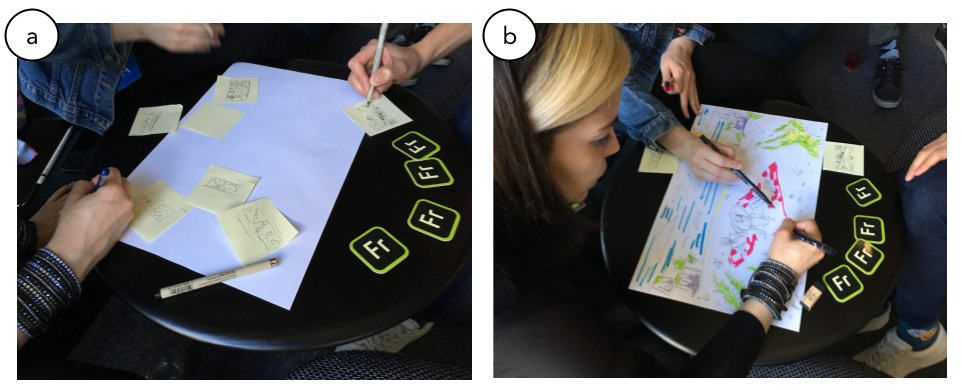
\includegraphics[width=\textwidth]{abstraction/figures/expert.png}
\vspace{-0.2in}
  \caption{a) Experts started planning by sketching multiple thumbnails that conveyed overall structure and composition more than details. b) These composition sketches provided a reference for experts during drawing.}
  ~\label{fig:expert}
  \vspace{-0.2in}
\end{figure}

``Blank page'' tools allow for open-ended abstraction, but are often unstructured. The problem with remaining too abstract or unstructured, especially in collaborative work, is that communication and consensus may get lost in the woods \cite{hinds1999curse,hinds2001}. Multiplayer experiences such as those in  Figma (www.figma.com), Google Docs \cite{wang2015students}, or collaborative drawing canvases (www.drawpile.net) enable a large range collaboration strategies, from allowing anyone to modify anything through pixel-perfect editing, to splitting the canvas or document into sections and assigning collaborators to each part. Digital whiteboards \cite{Ishii1992} and sketch interfaces \cite{lin2000denim} similarly give users the freedom to express their thoughts with as much or as little detail as desired. However, these systems leave it to the users to develop their own external collaboration structures. Without prerequisite knowledge of abstraction strategies, novices especially may continue to lean towards specific details, such as the exact specifications of a sketch \cite{welch2000sketching} or precise wording of an essay \cite{sommers1980revision}. Abstraction blocks ground the exploration and communication of abstract ideas to movable boxes to shift focus away from low-level details while giving tangible artifacts with which to interface.

\section{Interviews: Expert \& Novice Differences in Comic Drawing Process}
\label{sec:shown_ints} 

\subsection{Method: Interviewing Expert Artists \& Novices}
Differences in experts and novices have been well-studied in various domains from chess \cite{Chase1973} to physics \cite{chi1981categorization}; experts are able to contextually apply different high-level strategies to their work while novices often focus on details. We wanted to understand where novices struggle most in the domain of drawing comics to learn about the types of examples that would be most beneficial to support in an adaptive creativity support tool. 
We interviewed and observed nine expert artists and nine novices as they performed a comic-drawing task. We chose comics as a domain because most people would likely benefit from examples when engaging in the intersection of verbal and visual storytelling \cite{abel2008drawing,eisner2008comics, mccloud2006making} and because drawing comics requires only pen and paper at a minimum. 

We recruited experts from the freelance site Upwork, and novices through social media posts. Experts had formal art training and professional experience in making comic strips. We recruited novices who had a familiarity with comics, but no experience making comics and no formal education or professional experience in art. Over the course of an hour, participants drew a four-panel comic for one of three randomly given prompts: 

\begin{itemize}
\item{\textsc{Penguin}: a man befriends a penguin because of shared interests,}
\item{\textsc{Aliens}: aliens invade Earth during the 2020 global pandemic quarantine, and} \item{\textsc{Character}: a woman is upset at her date because he doesn't know who her favorite television or movie character is.} 

\end{itemize}
We asked participants to think aloud as they drew and asked questions about their process. After participants finished drawing, we asked them what they found easiest and hardest about making their comics, what the feel is the most important part of comics, and what type of help they feel would be most useful. All interviews took place on the Zoom video conferencing platform, and participants were allowed to draw digitally or use pen and paper. Experts received USD \$60 payment for their participation; novices received a \$25 gift card.

\begin{figure*}
  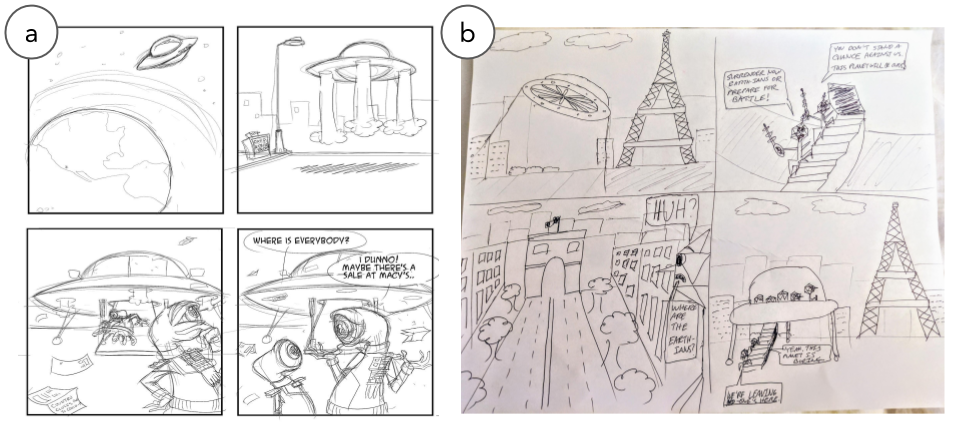
\includegraphics[width=\textwidth]{shown/figures/study1.png}
  \caption{Examples of an a) expert and b) novice comic for the \textsc{Aliens} prompt: aliens invade Earth during the 2020 global pandemic quarantine.}
  \label{fig:study1}
\end{figure*}

\subsection{Results}

\subsubsection{Experts Focus on Story \& Composition}
All nine expert artists expressed that story and composition are the most important parts of a comic: ``\textit{It’s all about composition because if you can’t understand how a comic moves, the narrative kind of decomposes}'' (Expert 4). Experts stressed that good drawing skills alone do not make a comic interesting, explaining that writing is more critical to a good comic than the fidelity of its drawings: ``\textit{I feel like the most important part is the composition of each panel because you can have great illustration..., but if the composition leads to just a random object in the background that isn’t important to the story..., the audience is going to miss something}'' (Expert 2).
Expert 8 similarly said, ``\textit{The most important thing is the writing because if you’re a good artist, but your writing stinks, you’re not going to make it. But you can have awesome writing and stick figures and make a million bucks, so to speak}.'' 

To achieve their narrative goals, experts mentioned using composition concepts and rules to help establish the flow and message of the comic. Expert 5 stated, ``\textit{There’s pretty simple rules of composition, you know, thirds, rhythm, all that stuff. They kind of help lead you to the subject’s eyelines.}'' As in prior work on expert drawing strategies \cite{Edwards1979,Poore1967}, experts drew rough sketches to rapidly outline their ideas. These quick sketches helped them evaluate their work in terms of visual concepts like composition, as well as narrative concepts like flow and pacing. For example, Expert 6 said, ``\textit{So I just plan out how I want it to look. And, you know, once you're done with something you're always like, ‘Oh, I can make that better. I can make it nicer.’ To get the general gist, we're going to see what they're doing, and etcetera.}'' Expert 1 similarly explained, ``\textit{And at this point, I'm still kind of planning stuff out. So I'm not really drawing what might be there, just kind of a reference. So I guess laying it out.}'' Three experts talked about typically creating thumbnail sketches to ideate panel compositions: ``\textit{I'll do like four or five different little sketches or thumbnails of what I think are good for the theme that I chose in my brainstorming session}'' (Expert 7). After a rough sketch, experts refine their sketch by adding in details, then move into a final inking stage to finish drawing their comic. Expert 5 said that doing a final drawing was the quickest part of the process because the idea in mind was already on paper. In general, experts spent most of their time on exploration and iteration while focusing on high-level elements like composition and flow, enabling them to finish drawing their comics quickly and simply. 

\subsubsection{Novices Focus on Details}
Verbally, novices also expressed the view that narrative arc is paramount: \textit{e.g.}, ``\textit{[The most important thing is] conveying the story I want to tell in as clear a way as possible}'' (Novice 8). Despite this, novices time allocation favored detailed drawings over composition and flow. For example, one novice drew the details of a character before deciding on story plot or composition. Another spent nearly 10 minutes drawing a person starting from the feet up in one panel, leading them to rush through subsequent panels: ``\textit{I’ve spent like 10 minutes on this, and I’m only on the feet!}'' (Novice 2)(Figure \ref{fig:novice}). In contrast to experts, novices often went straight into drawing their final comic with little conceptual planning or exploration. They were often hesitant to use sketches as exploratory tools and instead wrote out their ideas when conceptually planning their work: ``\textit{I know how to communicate my idea through words. That’s what I’m familiar with. I’m not as comfortable with drawing}'' (Novice 1). Conveying a clear story in the comic was the most important goal for all participants, but novices did not have an understanding of how to show their story visually. Figure \ref{fig:study1} shows an example of an expert and novice comic drawn for the \textsc{Aliens} story prompt. 

\begin{figure}
  \centering
  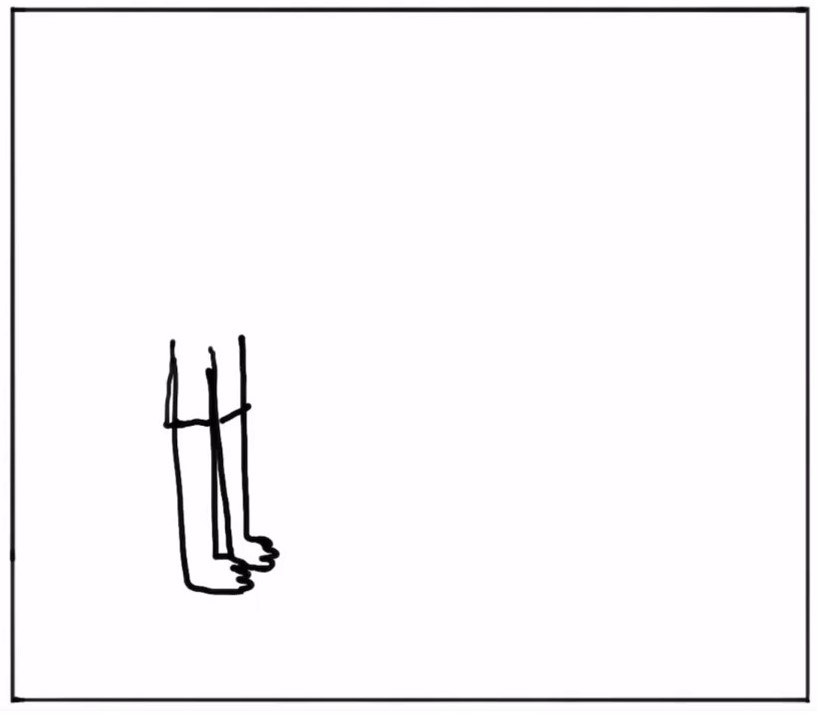
\includegraphics[width=.6\textwidth]{shown/figures/novice_detail.jpg}
  \caption{This novice from our interviews spent more than 10 minutes drawing a person from the feet up, fixating on getting the details of the character right.}
  \label{fig:novice}
\end{figure}

Interestingly, despite novices noting that narrative was the most important aspect of a comic, all novices attributed their inability to clearly tell a story to their lack of drawing skills. Novice 2 said, ``\textit{I can have an idea in my head, but actually translating it onto a comic is difficult.}'' Similarly, Novice 3 expressed that, ``\textit{I am able to visualize all of this very easily in my mind’s eye but everything else is kind of blank... It’s hard to translate that into a specific thing to draw because it’s not told to me what that might be.}'' When asked what help would be most useful for making their comic, seven of the nine novices said drawing help: ``\textit{I think generating the figures is something that could be automated, and [a computer] could have done a much better job than me}'' (Novice 7). Another expressed that drawing help would reduce tedium: ``\textit{I find drawing to be actually pretty tedious...if I could just come up with the panel and the script and give it someone or the computer that would be great}'' (Novice 6). The other two novices expressed a desire for templates or reference images to help them show their comic story.

The perceived lack of skill seemed to be a major factor in how novices chose compositions for their comic panels.
Novice 2 said, ``\textit{I'm thinking about what I want - like the image in my mind is literally what is on the square. And the way I decide what is on the square is because of my lack of drawing ability, it’s sort of like what is the simplest way that I can convey the message that I'm trying to set.}'' Exploring beyond the most achievable composition for a panel was also difficult: ``\textit{After you’ve decided on how to present the information or the previous information, and I feel like I don’t want to be repetitive..., and I didn’t know what would be the best way to draw my panel}'' (Novice 4). These observations highlighted two primary challenges for novices: 1) exploring ways to visually show their story idea, and 2) executing on that idea through drawing. Experts are able to quickly evaluate and decide upon alternatives through rough sketching whereas novices often fixate on making their single idea look an precise way. 

% As Jodi Picoult states, ``\textit{You can edit a bad page, but you can't edit a blank page}.''
\section{Guiding Drawing with Sh\"{o}wn}

Previous research in expert and novice differences find that novices focus on surface details and fixate on ideas \cite{Chase1973,chi1981categorization,jansson1991design,yuan2016}. Likewise, our observations showed that novices struggle with exploring alternative ideas and focusing excessively on details while drawing comics. We hypothesize that a system that helps novices consider and choose among options for \emph{what} to draw by presenting timely and relevant concepts and examples can help novices overcome these challenges as they work. 

Sch{\"o}n states that reflective practice is a continuous reframing and experimentation of ambiguous problems \cite{schon1984reflective}. Inspired by this articulation of reflective practice, we designed Sh{\"o}wn to explore our hypothesis. The Sh{\"o}wn Wizard-of-Oz system augments Google Jamboard, a web-based collaborative drawing tool, with two scaffolds for presenting examples: a drawing helper and adaptive conceptual guidance (Figure \ref{fig:shown}). We chose a Wizard-of-Oz method for two reasons: to study interaction recognition and contextual heuristics for presenting examples without the cost of full implementation, and to better observe how people used and applied conceptual examples \cite{walny2012understanding}. Because Google Jamboard is collaborative, the Wizard and the user can simultaneously see the other's activity by visiting the same link. This allows the Wizard to recognize the user's activity and provide assistance accordingly.

The Sh{\"o}wn interface comprises a drawing area for each comic panel, alongside selected examples. Users can flesh out panels in any order.
Following the drawing screens are a corpus of examples, adapted from McCloud's book \cite{mccloud2006making}, that show comic-specific concepts related to comic planning such as framing, transitions, and image and word combinations (Figure \ref{fig:shown}d). 
To communicate with the system, users can use voice commands or Jamboard's sticky notes feature to place notes on drawing screens. Sticky notes as an input mechanism allowed natural language text descriptions and deictic, ``put that there'' interactions \cite{engelbart1968research}.

\begin{figure}[t!]
  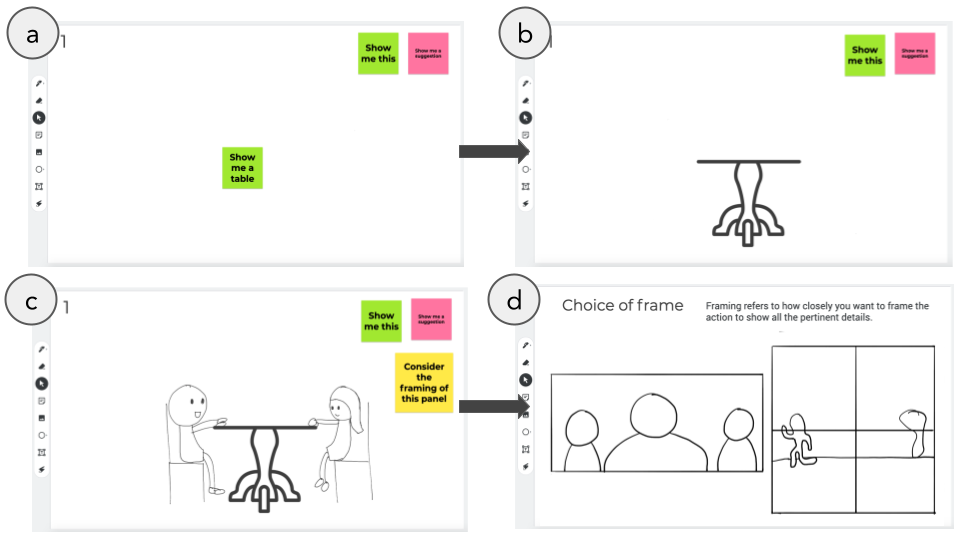
\includegraphics[width=\textwidth]{shown/figures/shown.png}
  \caption[Sh{\"o}wn’s interface and features.]{Sh{\"o}wn’s interface and features. a) A user wants to draw a comic panel showing a table and requests the drawing helper's assistance by typing a sticky note that says, ``Show me a table''. b) The drawing helper then provides a basic icon of the requested object in place of the sticky note request. c) As the user draws their panel, Sh{\"o}wn displays adaptive guidance on the right side of the screen in the form of a sticky note. d) The user can move to the immediate next screen to view relevant examples.}
  \label{fig:shown}
\end{figure}

\subsection{Adaptive Conceptual Guidance: Aiding Showing Relevant \\Examples at Relevant Moments}
We also found in interviews that, while novices enjoyed coming up with their own ideas and stories, they often did not know how to best visualize their ideas. To address this, Sh{\"o}wn provides adaptive conceptual guidance by first presenting high-level comic principles as a suggestion and then specific examples as the user works to inspire ideas for \emph{how} to portray their story. 
The guidance that Sh{\"o}wn currently provides is based on our interviews with experts and three concepts used by experts to decide how to convey a comic story \cite{abel2008drawing,eisner2008comics,mccloud2006making}: choice of framing, choice of moment or transition, and choice of images and words. McCloud \cite{mccloud2006making}, a comic expert and artist, writes that these concepts are part of the ``\textit{rough planning stage where a story’s events are first broken down into readable chunks}'' (\textit{pg. 11}). When presenting guidance, Sh{\"o}wn pairs an explanation of the concept with examples from McCloud’s book that show how the concept can be applied to a comic story.
(The concept of narrative flow is also mentioned in the book, but this refers to panel layout and spacing, which were not applicable to our study as we asked all participants to use the same four-panel layout.) Highlighting the concept behind examples reflects the scenario of an expert guiding a novice through a problem by explaining high-level concepts and providing specific instantiations of the concepts \cite{schon1984reflective}.

The timing of guidance is determined by the following set of recognition heuristics with three principles in mind based on prior work: examples should be related to what the user is currently doing \cite{fraser2019replay,kandel2011wrangler,kumar2011, Lee2010, ngoon2018interactive}, examples should be shown as early in the creative process as possible \cite{kulkarni2012early,Siangliulue}, and examples should be paired with an explanation of the underlying concept they illustrate \cite{javadi2012impact,ngoon2018interactive}.
\\
The three types of guidance that Sh{\"o}wn supports are:

\textbf{Consider the framing for this panel.} Framing refers to composition or use of camera angle and distance to show pertinent actions or details in the panel. This guidance is often presented on the first panel before a user begins drawing to help them get started with their comic. If the user is drawing a subsequent panel, Sh{\"o}wn presents this guidance if the panel’s framing is repeated from any previous panels (\textit{e.g.} if the user begins to use a medium shot in the second panel after using the same camera angle/shot in the first panel). 

\textbf{Consider the moment or transition between panels.} Moment or transition refer to the continuity between actions in panels and the specific moments shown as part of the story in each panel. This guidance is presented when a user moves to a new panel to help them think of transitions between panels.

\textbf{Consider the combination of images and words in this panel.} The combination of images and words refers to how words and images together can tell story more powerfully than either alone. This guidance is presented if the images between panels are similar, if a panel contains a lot of or no text or dialogue, or if the user is attempting to draw facial expressions. 

\subsection{Adaptive Conceptual Guidance in Action}
While the user is drawing their comic, the Wizard is simultaneously using the same prototype link to provide guidance to the user. As the user is drawing their comic, Sh{\"o}wn adaptively displays one of the three guidance suggestions based on the user’s current task and context. The Wizard displays guidance ambiently \cite{matejka2011ambient} on the right side of the panel page without interruption to the user via the sticky notes tool (Figure \ref{fig:shown}c). For instance, a user is drawing the same composition for two panels, in which two people are sitting at a table in the center of the page. Because of the repeated framings, the Wizard presents guidance for the user to ``\textit{consider the framing of this panel}'' in the form of a sticky note that is added to the right side of the drawing screen (Figure \ref{fig:shown}c) to provide inspiration for alternative ways of composing the panel. When the user sees the suggestion and clicks on the sticky note, the Wizard displays a specific example screen that shows examples corresponding to the concept being presented (Figure \ref{fig:shown}d). The user can then return to their drawing screen and modify their drawing if they choose. When the user moves to the next panel, the Wizard presents guidance for the user to ``\textit{consider the moment or transition between panels}'' before the user begins to draw their panel. After clicking on the sticky note, the Wizard presents examples showing different ways to use pacing in a comic narrative. Users can also proactively ask for guidance at any point by clicking the ``Show me a suggestion'' sticky note on the right side of any drawing screen. Users can also ignore guidance if they choose.

\subsection{The Drawing Helper: Freeing Focus from Detail}
In our interview study, novices experienced difficulty in executing their ideas and overly focused on details due to a lack of confidence in their drawing skills. To mitigate this and enable a larger focus on story, Sh{\"o}wn provides a drawing helper that can automatically render a basic sketch of a requested object using Google Jamboard's Autodraw feature, which presents icons that match the sketch input. We differentiate these icons from examples presented in adaptive conceptual guidance as these are basic renderings of objects rather than conceptual examples. If the options provided by Autodraw were not sufficient, the human Wizard provided a simple drawn sketch. The drawing helper was designed to draw basic objects such as a table or person rather than complex characters or scenes. For instance, a user wants to draw a comic story about two people having a dinner date. They want to draw the couple sitting at a table, but don't want to focus on the details of the table itself. The user asks the drawing helper for a table by making a sticky note with the text ``\textit{show me a table},'' and placing it in the center of the drawing screen (Figure \ref{fig:shown}a). The Wizard then produces an icon of the table in the location specified by the user (Figure \ref{fig:shown}b). Later, the user wants a drawing of a chair and this time requests an example via voice command by saying ``show me a chair.'' Sh{\"o}wn renders an icon of a chair, and the user can move the chair to where they desire on the screen. The drawing helper provides simple drawing objects so the user can then focus their attention on utilizing the conceptual examples that support the high-level narrative aspects of their comic story.
\section{Experiment}
\label{sec:shown_exp}
We wanted to test the hypothesis that a creativity support tool that offers adaptive conceptual guidance would help novices better utilize examples and improve creative outcomes than a tool that only provides non-adaptive examples.

\subsection{Method}

\subsubsection{Participants}
We recruited 24 novice participants (9 male, 15 female, median age = 22) through social media, mailing list advertisements, and the site UserTesting to evaluate our Wizard-of-Oz system. Similar to our interviews, we recruited novices that had familiarity with comics, but no formal education in art or professional experience in making comics. We also required participants to draw using a digital tablet with a stylus for ease of drawing. Half the participants were randomly assigned to the \textit{non-adaptive} condition while the other half was assigned to the \textit{adaptive} condition. The task asked participants to make a rough draft of a four-panel comic based on a randomly-assigned prompt from the interview study (\textsc{Penguin}, \textsc{Aliens}, or \textsc{Character} prompts). Four participants from each condition saw each of the three prompts. We encouraged black-and-white comics for simplicity, but using color was allowed. All one-hour sessions took place on the Zoom video conferencing platform, and participants received a USD \$25 gift card for their participation. 

\subsubsection{Procedure}
At the start of each study session, participants received a link to Sh{\"o}wn on Google Jamboard and were given a tutorial from the experimenter about Sh{\"o}wn’s features. \textit{Adaptive} condition participants created their comic in a version of Sh{\"o}wn with adaptive conceptual guidance where conceptual examples were presented selectively based on the heuristics described earlier. \textit{Non-adaptive} condition participants used an otherwise identical version of Sh{\"o}wn without adaptive conceptual guidance (the same conceptual examples were available via the example screens, but not selectively presented, similar to previous work with example galleries). All participants had access to the drawing helper because our main research question was about adaptive conceptual guidance versus non-adaptive examples. We chose to include the drawing helper for both conditions because Google Jamboard's Autodraw feature, which is the engine behind the drawing helper's icons, already exists within the tool itself.
Participants spent up to an hour drawing their comic while using a think-aloud protocol \cite{ericsson1984protocol}. At the end of the study session, participants answered post-interview questions about their process and thoughts on Sh{\"o}wn’s scaffolds. Following the study, we debriefed participants to inform them about the Wizard-of-Oz nature of the study.

\subsubsection{Measures}
We measured participants' behaviors and interactions with Sh{\"o}wn's features, such as the number of times participants used the drawing helper, viewed examples, and verbally expressed implementing concepts from the examples. We determined whether participants implemented examples either by their verbal expression of doing so or if they changed their panel after viewing examples. We also measured creative outcomes by gathering quality ratings of each comic from lay readers. We chose lay readers as raters (rather than experts) because lay readers are a large audience for comics, and because we wanted to capture overall story impact rather than technical quality, in line with the focus of both experts and novices in our interview study on narrative clarity.

Specifically, we measured comics in terms of clarity, creativity, and overall preference. In pairwise comparisons, raters from Mechanical Turk (61 unique Mechanical Turk workers) were sequentially presented with a pair of comics (two comics for the same prompt, one from each condition). For each pair, raters selected which comic they believed had more unique drawings and a more unique story (creativity), which comic had clearer drawings and a clearer story (clarity), and which comic they preferred overall. We separated drawing measures from story measures to account for potential individual differences in drawing ability. Pairing one comic from each condition for each prompt yielded 48 unique pairs (four \textit{non-adaptive} comics $\times$ four \textit{adaptive} comics $\times$ three prompts). Workers were paid USD \$1 to rate five pairs in sequence. Every pair received evaluations from at least five different raters, resulting in 306 total ratings.

\subsection{Results}

\begin{figure*}
  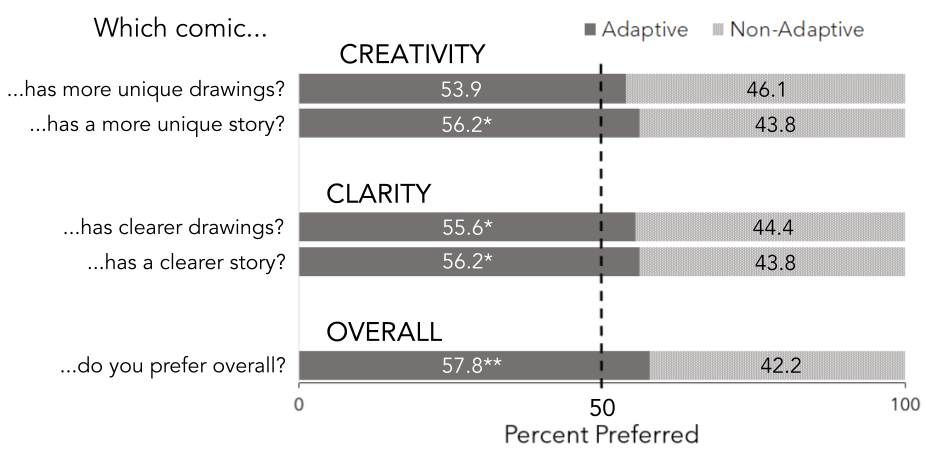
\includegraphics[width=\textwidth]{shown/figures/woz-results.png}
  \caption[\textit{Adaptive} condition ($n=12$) comics received significantly more preference ratings for more unique stories ($\chi^2=5.12, df=1, p<.05$), clearer drawings($\chi^2=3.91, df=1, p<.05$), clearer story ($\chi^2=5.12, df=1, p<.05$), and overall preference ($
\chi^2=7.87, df=1, p<.01$)]{\textit{Adaptive} condition ($n=12$) comics received significantly more preference ratings for more unique stories ($\chi^2=5.12, df=1, p<.05$), clearer drawings($\chi^2=3.91, df=1, p<.05$), clearer story ($\chi^2=5.12, df=1, p<.05$), and overall preference ($
\chi^2=7.87, df=1, p<.01$) than \textit{Non-adaptive} condition ($n=12$) comics. $*p<.05, **p<.01$}
  \label{fig:woz}
\end{figure*}

\subsubsection{Raters Preferred Adaptive Condition Comics Overall and for Most Other Measures}
Raters preferred \textit{adaptive} comics significantly more often than \textit{non-adaptive} comics overall (\textit{adaptive}=57.8\%, \textit{non-adaptive}=42.2\%, $
\chi^2=7.87, df=1, p<.01$) (Figure \ref{fig:woz}). In terms of clarity, raters preferred \textit{adaptive} comics more often when asked which had clearer drawings (\textit{adaptive}=55.6\%, \textit{non-adaptive}=44.4\%, $\chi^2=3.91, df=1, p<.05$) and which had clearer stories (\textit{adaptive}=56.2\%, \textit{non-adaptive}=43.8\%, $\chi^2=5.12, df=1, p<.05$). \textit{Adaptive} comics were also more often preferred when raters were asked which had more unique stories (\textit{adaptive}=56.2\%, \textit{non-adaptive}=43.8\%, $\chi^2=5.12, df=1, p<.05$). There was no significant difference in preference ratings for which comic had more unique drawings (\textit{adaptive}=53.9\%, \textit{non-adaptive}=46.1\%, $\chi^2=2.19, df=1, p=.14$). 
Figure \ref{fig:preferred} shows the most preferred comic for each measure as rated by the MTurk workers.

\subsubsection{Adaptive Conceptual Guidance Made Examples More Useful}
Sh{\"o}wn presented guidance at least three times to each \textit{adaptive} participant per session with a maximum of six times ($M=3.92$, $SD=0.90$). All \textit{adaptive} participants viewed at least one example screen at least one time while drawing, with an average of three times per session ($SD=1.13$). \textit{Adaptive} participants verbally expressed implementing concepts from examples an average of 2.17 times per session  ($SD=1.11$). In contrast, three \textit{non-adaptive} condition participants viewed examples, with an average of 0.67 examples viewed per session ($SD=1.23$)($t=4.84$, $df=21.8$, $p<.001$). 

\textit{Adaptive} participants mentioned that guidance served as inspiration, helping them think of new ways of showing their story they would not have otherwise realized. For example, P5 (\textit{adaptive}) noted, ``\textit{As I was going through I think I got into the same rhythm of what I wanted to show, and I think the [guidance] made me more cognizant of ways that I could switch things up. Like I don't think I would have thought of this last panel if I didn't get a nudge from those.}'' P16 (\textit{adaptive}), whose comic was the most preferred overall and for the most unique story, similarly stated, ``\textit{I think the [guidance] helped me consider different things. For example, for the 3rd panel, I wouldn't have considered doing a shot from the back of his head to show [the woman’s] point of view}'' (Figure \ref{fig:p16}). For the \textit{non-adaptive} participants who did view the examples, they also served as inspiration. P21 (\textit{non-adaptive}), whose comic was most preferred for having unique drawings, also cited the examples as helpful for their comic: ``\textit{[The examples] were kind of like a guide to give me a vocabulary for my intentions}.''

\begin{figure}[t]
  \hspace*{-1cm}%
  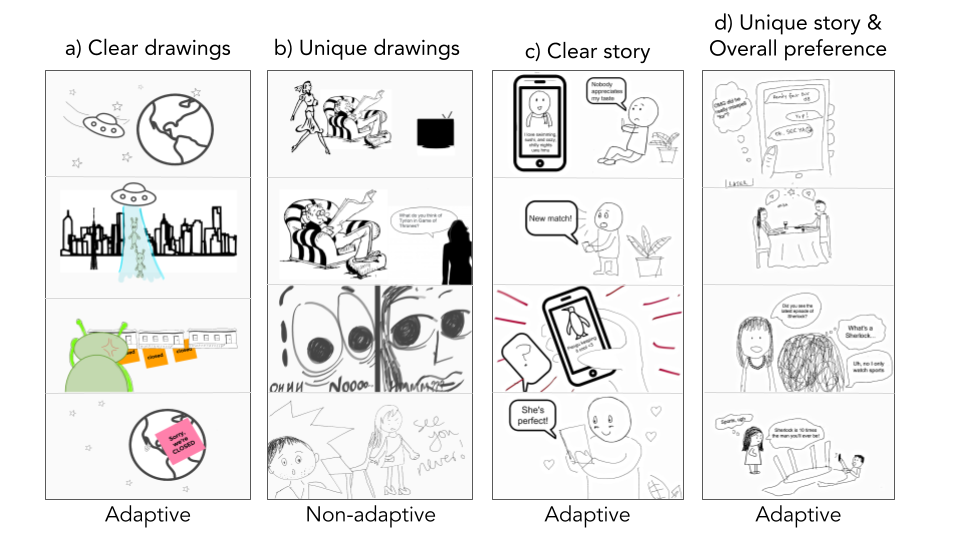
\includegraphics[width=\dimexpr\textwidth+2cm\relax]{shown/figures/preferred.png}
  \hspace*{-1cm}%
  \caption{The most preferred comics for each measure of clear drawings, unique drawings, clear story, unique story, and overall preference.}
  \label{fig:preferred}
\end{figure}

However, some \textit{non-adaptive} participants did not believe the examples were applicable. For example, P18 (\textit{non-adaptive}) stated, ``\textit{I already had an idea in mind so I didn’t really need the examples.}'' P15 (\textit{non-adaptive}) forgot the examples were available but wished he had used them after finishing his comic: ``\textit{I think I should have looked at [the examples] before I started drawing}.'' Similarly, although participants could proactively ask for guidance in the \textit{adaptive} condition, only two participants did so. One participant mentioned that he ``\textit{just wanted to see what suggestions were available}'' (P14, \textit{adaptive}). 

\subsubsection{Participants Wanted More Understandable Heuristics for Adaptive Conceptual Guidance}
The Wizard uses specific heuristics for displaying guidance. However, the heuristics Sh{\"o}wn used to decide when to show guidance, even if slightly off, could diminish the effectiveness of examples. Most felt the real-time guidance was useful: ``\textit{[The suggestions] were like a guidance for me. I don’t think I would go look at [the examples], so it was nice that they were shown throughout the drawing part}'' (P10, \textit{adaptive}). 
However, one participant wished guidance was presented at the beginning of drawing: ``\textit{I think these come a bit too late for me to use them because they're sparsed in between while I'm drawing. For example, the perspective one, I thought `oh, I should've used this earlier,' but the information just came a bit too late for me to use}'' (P6, \textit{adaptive}). 
This suggests that guidance heuristics should not be ``one-size-fits-all'' but rather allow users to adjust them based on perceived usefulness.

Some \textit{adaptive} participants also thought the timing and reasoning for presenting certain guidance was opaque. 
They wanted to know more about why particular advice was being given at a particular moment. P24 (\textit{adaptive}) stated, ``\textit{The suggestions were helpful, but it wasn't clear why that suggestion was being given. Like for the transition one, it could be that my transition isn't the best one I could use for my viewer or it could just be helping me get started so it wasn't clear why it was giving me those suggestions}.''
While adaptive conceptual guidance helped participants better understand examples, clarity around what the system is responding to would help users decide between many possible valid uses of those examples.

\begin{figure}[b!]
  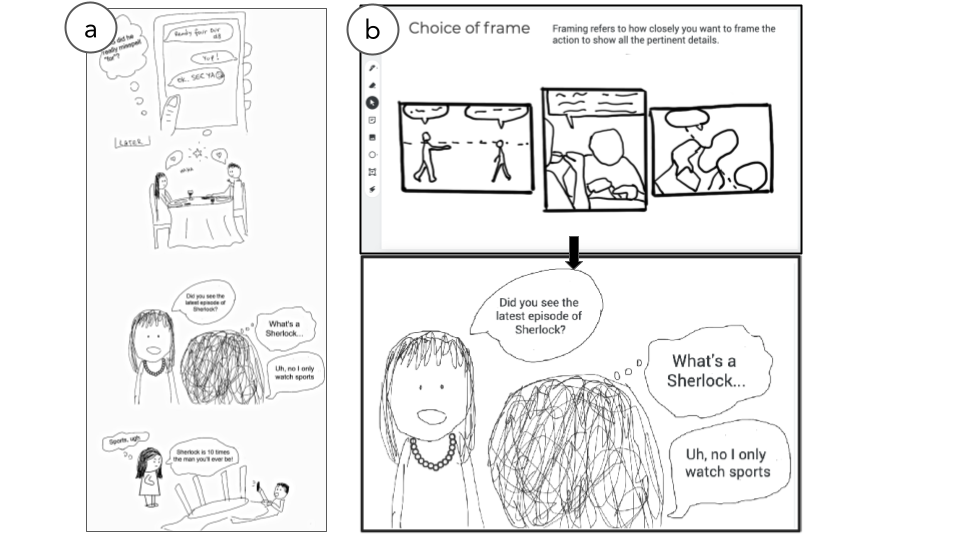
\includegraphics[width=\textwidth]{shown/figures/p16.png}
  \caption{a) This comic was created using Sh{\"o}wn's adaptive conceptual guidance. b) The participant cited that seeing a relevant example inspired the composition of the third panel of the comic.}
  \label{fig:p16}
\end{figure}

\subsubsection{The Drawing Helper Shifted Focus from Details to Story}
We tracked user interactions with the drawing helper to understand how people used this feature and how it possibly interacted with example use. Participants in both conditions used the drawing helper frequently, with an average of 4.67 times ($SD=2.87$) per session for \textit{adaptive} participants and 5.67 times ($SD=4.68$) for \textit{non-adaptive} participants ($t=-0.63$, $df=18.3$, $p=.54$). In some cases, the drawing helper made drawing objects---particularly repeated objects---less tedious. For example, P24 (\textit{adaptive}) used the drawing helper to draw a phone screen that would be consistent across all panels. P11 (\textit{non-adaptive}) felt the drawing helper did indeed help him focus less on details: ``\textit{I thought [the drawing helper] was really cool, especially for like tables or chairs or to hash out the overall setting so you can just focus on the other stuff.}'' P21 (\textit{non-adaptive}) thought the drawing helper was useful for showing her intended vision: ``\textit{I could just tell [the drawing helper] my vision, and it would bring up things that are relevant}.'' 
Our findings suggest that the concreteness provided by tools like the drawing helper may complement the efficacy of strategies like adaptive conceptual guidance. 

However, a few participants felt limited in their creativity with the drawing helper. One participant noted an over-reliance on the drawing helper rather than sketching, stating, ``\textit{I kinda became too dependent on [the drawing helper]. Normally, I would just draw it out quickly, but I want to see what the system can do...With the tool, I think if the system can do this for me, and it's perfect the first time, I try to see how I can fit my idea to what the system can do}'' (P15, \textit{non-adaptive}). 
Another participant felt that the simplicity of the drawing helper's sketches did not allow them to completely show their vision: ``\textit{It was pretty limited in what it could show. Like I couldn't do perspectives or angles with the basic icons I was given}'' (P12, \textit{adaptive}). 
These observations corroborate the fact that we found no significant difference in visual creativity across the two conditions ($\chi^2=2.20, df=1, p=.14$).
Three participants did not use the drawing helper or only used it once because, as one participant stated, ``\textit{It might have been more helpful if I was drawing something more complex, but it was just easier to draw it on my own}'' (P13, \textit{non-adaptive}). 
\section{Discussion \& Future Work}
This chapter investigated whether providing adaptive conceptual guidance aids example use more effectively than non-adaptive examples through a Wizard-of-Oz prototype and empirical study. We next discuss implications of our findings for future creativity support tools and generalization to other domains. 

\subsection{System-Directed Versus User-Directed Creativity Support}
In our experiment, we observed that novices in both conditions rarely sought examples without being prompted, perhaps because they were unaware of needing help or did not know what help they needed. Only two \textit{adaptive} condition participants proactively asked for guidance, and only three \textit{non-adaptive} condition participants viewed the examples gallery on their own. While exploring alternatives is a useful problem-solving strategy, meaningfully evaluating them requires expertise and the comparison induces a hefty cognitive load \cite{tuovinen1999comparison}. In line with prior work \cite{bilalic2008good, Graesser1994,Siangliulue}, this suggests that timing is relevant to giving the most appropriate help as novices may not know what type of help is most helpful and when. By incorporating concepts with examples, we found that Sh{\"o}wn's real-time adaptive conceptual guidance helped to expand participants' field-of-view to concepts they would not have known to explore on their own. Such proactive system-directed approaches seem to benefit open-ended creative problems (like figuring out how to draw a comic story) because they help users explore beyond known possibilities.

Similar to other systems that present galleries of examples to provide broad inspiration \cite{kang2018paragon,Lee2009,marks1997design}, Sh{\"o}wn provides high-level examples meant for conceptual exploration rather than examples that are particular to the user's specific work. For example, if a user wants to draw two people talking, Sh{\"o}wn presents general examples of different panel framings or combinations of text and images rather than specific instances of two people talking in a panel. These context-agnostic examples are framed as considerations (rather than statements that impose specific approaches as the ``correct'' ones). This open-ended approach is analogous to human tutoring, where less didactic interactions allow the learner to form their own explanations and hypotheses in evaluating ideas \cite{Chi2010}. 
In addition, recommending guidance in-situ allowed participants to better understand the relevance of guidance and evaluate examples in context \cite{schon1984reflective}. One participant explicitly mentioned that showing guidance in the moment while drawing encouraged them to view the examples when they would not have otherwise. Participants cited that even if they did not change their initial idea, the provided examples served as inspiration or as a way to help them explain their choices. In these instances adaptive conceptual guidance seemed to serve as a nudge for users to consider different options or evaluate their own decisions. 

In contrast, user-directed approaches (such as query-based systems and other help-seeking tools \cite{fraser2019replay,Huang2019, Satyanarayan2014}) seem to work best when the user has a concrete idea they want to execute. We saw this with how participants made use of Sh{\"o}wn's drawing helper, which produced basic icons to quickly visualize ideas based on a user's request. Some used voice commands to direct the drawing helper to provide images. However, the drawing helper had its limits: it could not generate drawings in response to complex, ambiguous requests. For example, P15 (\textit{non-adaptive}) asked the drawing helper to lay out an entire panel: ``\textit{Show me a man holding a phone with a dating app on it and lists for interests.}’’ 
This participant attempted to shape their ideas around what the drawing helper could generate, rather than using it to show their own ideas. This reflects how novices may form an over-reliance on help-tools or conform to salient features rather than high-level considerations \cite{jansson1991design,javadi2012impact,marsh1996examples,Smith1993}. Our findings with Sh{\"o}wn suggest that user-directed guidance works best for small and concrete tasks where the user already has an idea in mind.

Both system-directed and user-directed guidance can support the creative process in complementary ways. Context-agnostic conceptual aid allows for the ambiguity of exploration while specific user-directed guidance can give a concrete direction towards accomplishing goals. In many ways, using examples as guidance is similar to coaching or tutoring, where a coach or tutor gives both open-ended hints or suggestions and concrete examples depending on a person's progress. Sh{\"o}wn provides a demonstration of using context from user actions to leverage such guidance for creative work. Future research could further examine how computational systems can provide more adaptive coaching or tutoring for creative endeavors.

% limitations of current study
\subsection{Designing Adaptive Conceptual Guidance Systems: Limitations \& Opportunities}
We found two areas where adaptive conceptual guidance could be improved. The first is in determining the timing of guidance. One participant felt that guidance was presented too late and would be more helpful or more relevant earlier. While guidance was shown adaptively, the heuristics for determining when to show certain concepts and examples were static for each participant, which is both a limitation of the Wizard-of-Oz implementation as well as potential technical implementations. One open question is how to better anticipate when to provide guidance when even the user does not know when to ask for help. Potential effective timing mechanisms might be measuring how long a user is idle \cite{chan2018best,Siangliulue} or taking a mixed-initiative approach in incorporating user input, such as refining or pruning suggestions \cite{kandel2011wrangler} to determine the best moments to present examples. 

The second area of improvement is providing transparency around why guidance was being given. Three participants wanted further explanation for why certain pieces of guidance were being shown at specific times. One participant asked the experimenter whether the system presented guidance randomly or not. Another thought the presentation of guidance meant the system did not ``like'' their current drawing. This sentiment reflects prior work showing that people prefer explainable and transparent interactions with AI systems so they not only understand what help is being given but also why \cite{Amershi,Heer2019,Oh2018}. One possibility is to display guidance alongside interactive checkboxes or dynamic rubrics to help users understand how to better situate guidance within the user’s context \cite{Bharadwaj,ngoon2018interactive}.

We also found potential in improving user-directed support. While participants did not often explicitly seek out examples while working on their comics, many participants in both our interviews and experiment asked ideation questions aloud such as ``\textit{How do I show this place is empty?}'' or ``\textit{How do I show that this character is angry?}'' as part of the think-aloud protocol. These questions could serve as queries to indicate user intent and aid in tailoring the type of examples shown. During exploratory tasks like brainstorming ideas or deliberating ways to translate an idea visually, users may have more of these open-ended queries in mind rather than concrete goals. Tools that adaptively display help for just-in-time learning as well as incorporate contextual search mechanisms like natural language and deictic instructions may be useful ways of enabling user-directed conceptual support \cite{fraser2020remap, Graesser2001, laput2013pixeltone, Yoon}. 

%limitations of system design
As a Wizard-of-Oz prototype, Sh{\"o}wn utilizes a human Wizard to use a user's actions as heuristics to determine what conceptual guidance to provide. Some of the heuristics were based simply on starting on new panels (\textit{i.e.} the Wizard shows the guidance to consider moments or transitions when the user moves on to a new panel). Other heuristics were based on capturing the user's past and current actions (\textit{i.e.} the Wizard presents guidance on images and words if the panel contained too much or too little text). Existing tools already use sketch-based actions as context such as Procreate's Quick Shape tool\footnote{https://procreate.art/handbook/procreate/guides/quickshape//} to automatically complete shapes or straighten a user's lines or Google Jamboard's Autodraw tool that uses object recognition to infer what icons to suggest to the user. Co-creative intelligent agents can also use object and line recognition to improvise collaborative drawing \cite{Davis2016}. Our Wizard-of-Oz evaluation shows how adaptive systems might use visual, sketch-based context to provide conceptual guidance beyond automated drawing help or example galleries. Open remaining questions are how systems might be trained to learn such context as well as what types of context and concepts are most appropriate for adaptive and automated assistance beyond sketching.

One limitation of Sh{\"o}wn was that the example screens were separate from the drawing screens, requiring users to switch between drawing and example screens in order to view them. Tools incorporating adaptive conceptual guidance or examples presentation should consider more ambient displays that show examples without requiring the user to change the context of their work. Because of the remote nature of the study, one limitation was that we could not control for the screen size participants used. This may have affected drawing ability, though this limitation may have been mitigated since all participants used a stylus and had the drawing helper available.

Tools that help novices overcome skill barriers to execute their creative goals are powerful, but without seeing potential alternatives and possibilities, novices remain bounded by their limited conceptual expertise. Sh{\"o}wn evaluates simple recognition heuristics through a Wizard-of-Oz implementation to contextually present concepts and examples for better exploration and execution. Future work could examine feasibility and implementation of such heuristics for creativity systems across domains. We find that combining user-led support for concrete queries and adaptive support for open-ended exploration of alternatives helps novices better understand and utilize alternatives for their own work. An interleaving of system-led support and user-led agency is a promising direction for the development and evaluation of future creative tools \cite{Heer2019}. We provide a demonstration of this direction that can apply to creative endeavors across domains.

\subsubsection{Summary}
% do this for all chapters
We present Sh{\"o}wn, a Wizard-of-Oz system that provides adaptive conceptual guidance by suggesting relevant concepts and examples for a user to explore based on their current task. We hypothesized that adaptive conceptual guidance would guide the application of examples and improve creative work more than simply providing static examples alone. Through interviews and a between-subjects experiment in the domain of comics, we found that adaptive conceptual guidance led to comics with more unique and clear stories and clearer drawings. Users also found adaptive conceptual guidance to be timely and useful for inspiration while users without guidance did not find the examples as relevant and were less likely to take advantage of them. We argue for tools that help novices explore ideas by providing the right kinds of assistance in the right situations. In this way, we may better expand novices' vantage points to explore concepts more broadly and improve creative work. This chapter provides a direction for the future of adaptive creativity support tools and presentation of examples.

\subsubsection{Acknowledgements}
We thank the novice and expert comic artists for participating in interviews and our experiment participants for their time and efforts. This research was funded in part by Adobe Research.

This chapter, in part, includes  portions of material as it appears in \textit{Sh\"{o}wn: Adaptive Conceptual Guidance Aids Example Use in Creative Tasks} by Tricia  J. Ngoon, Joy O. Kim, and Scott Klemmer in the Proceedings of the 2021 ACM Conference on Designing Interactive Systems (DIS '21). The dissertation author was the primary investigator and author of this paper.

\chapter{CritiqueKit: Interactive Guidance Techniques for Improving Creative Feedback}
\label{chapter:critiquekit}
\begin{quote}
    Good feedback is critical to creativity and learning, yet rare. Many people do not know how to actually provide effective feedback. In providing feedback novices tend to focus on low-level, superficial details, leading to lower quality feedback. This chapter introduces two interactive techniques for improving feedback in creative work: reusable suggestions and adaptive guidance. These techniques are embodied in the CritiqueKit system to help reviewers give specific, actionable, and justified feedback. Two real-world deployment studies and two controlled experiments with CritiqueKit found that adaptively-presented suggestions improve the quality of feedback from novice reviewers. Reviewers also reported that suggestions and guidance helped them describe their thoughts and reminded them to provide effective feedback.

\end{quote}

\section{Introduction: Feedback's Hidden Potential}
Feedback is one of the most powerful influences on learning and achievement \cite{Hattie2007}. Both giving and receiving formative feedback encourage self-reflection and critical thinking on one's work \cite{Li2010, Nicol2006}, especially in creative and open-ended domains such as design and writing \cite{Hattie2007, sadler1989formative}. The growing scale of many educational and professional settings increases both the importance and difficulty of providing sufficiently descriptive and personalized feedback. Good feedback can be hard to generate, and people are not consistently skilled in doing so \cite{kulkarni2013peer, yuan2016}. Feedback is often too short, vague, and not actionable \cite{Kulkarni2015, sommers1980revision, Xiong2012}. Even experienced reviewers don't always recognize when they are providing poor feedback or why it is ineffective \cite{sommers1980revision}.

This chapter contributes two interactive techniques that improve feedback in the moment, their embodiment in the CritiqueKit system, and their evaluation through two deployments and two experiments.

\textbf{Interactive guidance of feedback characteristics.} CritiqueKit features a guidance panel with checkboxes that update as the reviewer gives feedback. A text classifier categorizes feedback as Specific, Actionable, and/or Justified as the reviewer types, providing them with an ambient awareness of their feedback quality and guiding them to improve their feedback in real-time while writing.

\textbf{Suggesting prior feedback for reuse.} CritiqueKit enables reviewers to reuse expert feedback, reducing experts' labor by scaling their feedback to similar work. These suggestions update and adapt based on the feedback's categorization to give reviewers targeted ideas for how to improve their comment and provide inspiration. 

Two deployment studies and two controlled experiments investigated the efficacy of these interactive techniques on the quality and characteristics of feedback. The first deployment examined how experienced reviewers (teaching assistants) reuse feedback in an undergraduate course. The second deployment examined how undergraduate students reuse feedback. The first experiment examined the impact of statically presented suggestions and interactive guidance on novice feedback. Finally, the second experiment examined the efficacy of adaptively updating suggestions in tandem with interactive guidance on novice feedback. We found that adaptively-presented suggestions improved feedback quality. Reviewers found suggestions useful for inspiration, and the interactive guidance reminded them to ensure their comments met the criteria for effective feedback. This work provides evidence that interactive techniques such as suggestions and guidance can effectively scaffold the feedback process, improving the feedback people give without needing them to spend extensive time learning good techniques (See Table \ref{table:critiquekit_all_results} for details).

\begin{table}[t]
\centering
  \caption{Two deployments (DEP) and two between-subjects experiments (EXP) examined the efficacy of feedback reuse and interactive guidance. We found that interactive suggestions and guidance were most helpful for improving feedback.}~\label{table:critiquekit_all_results}
  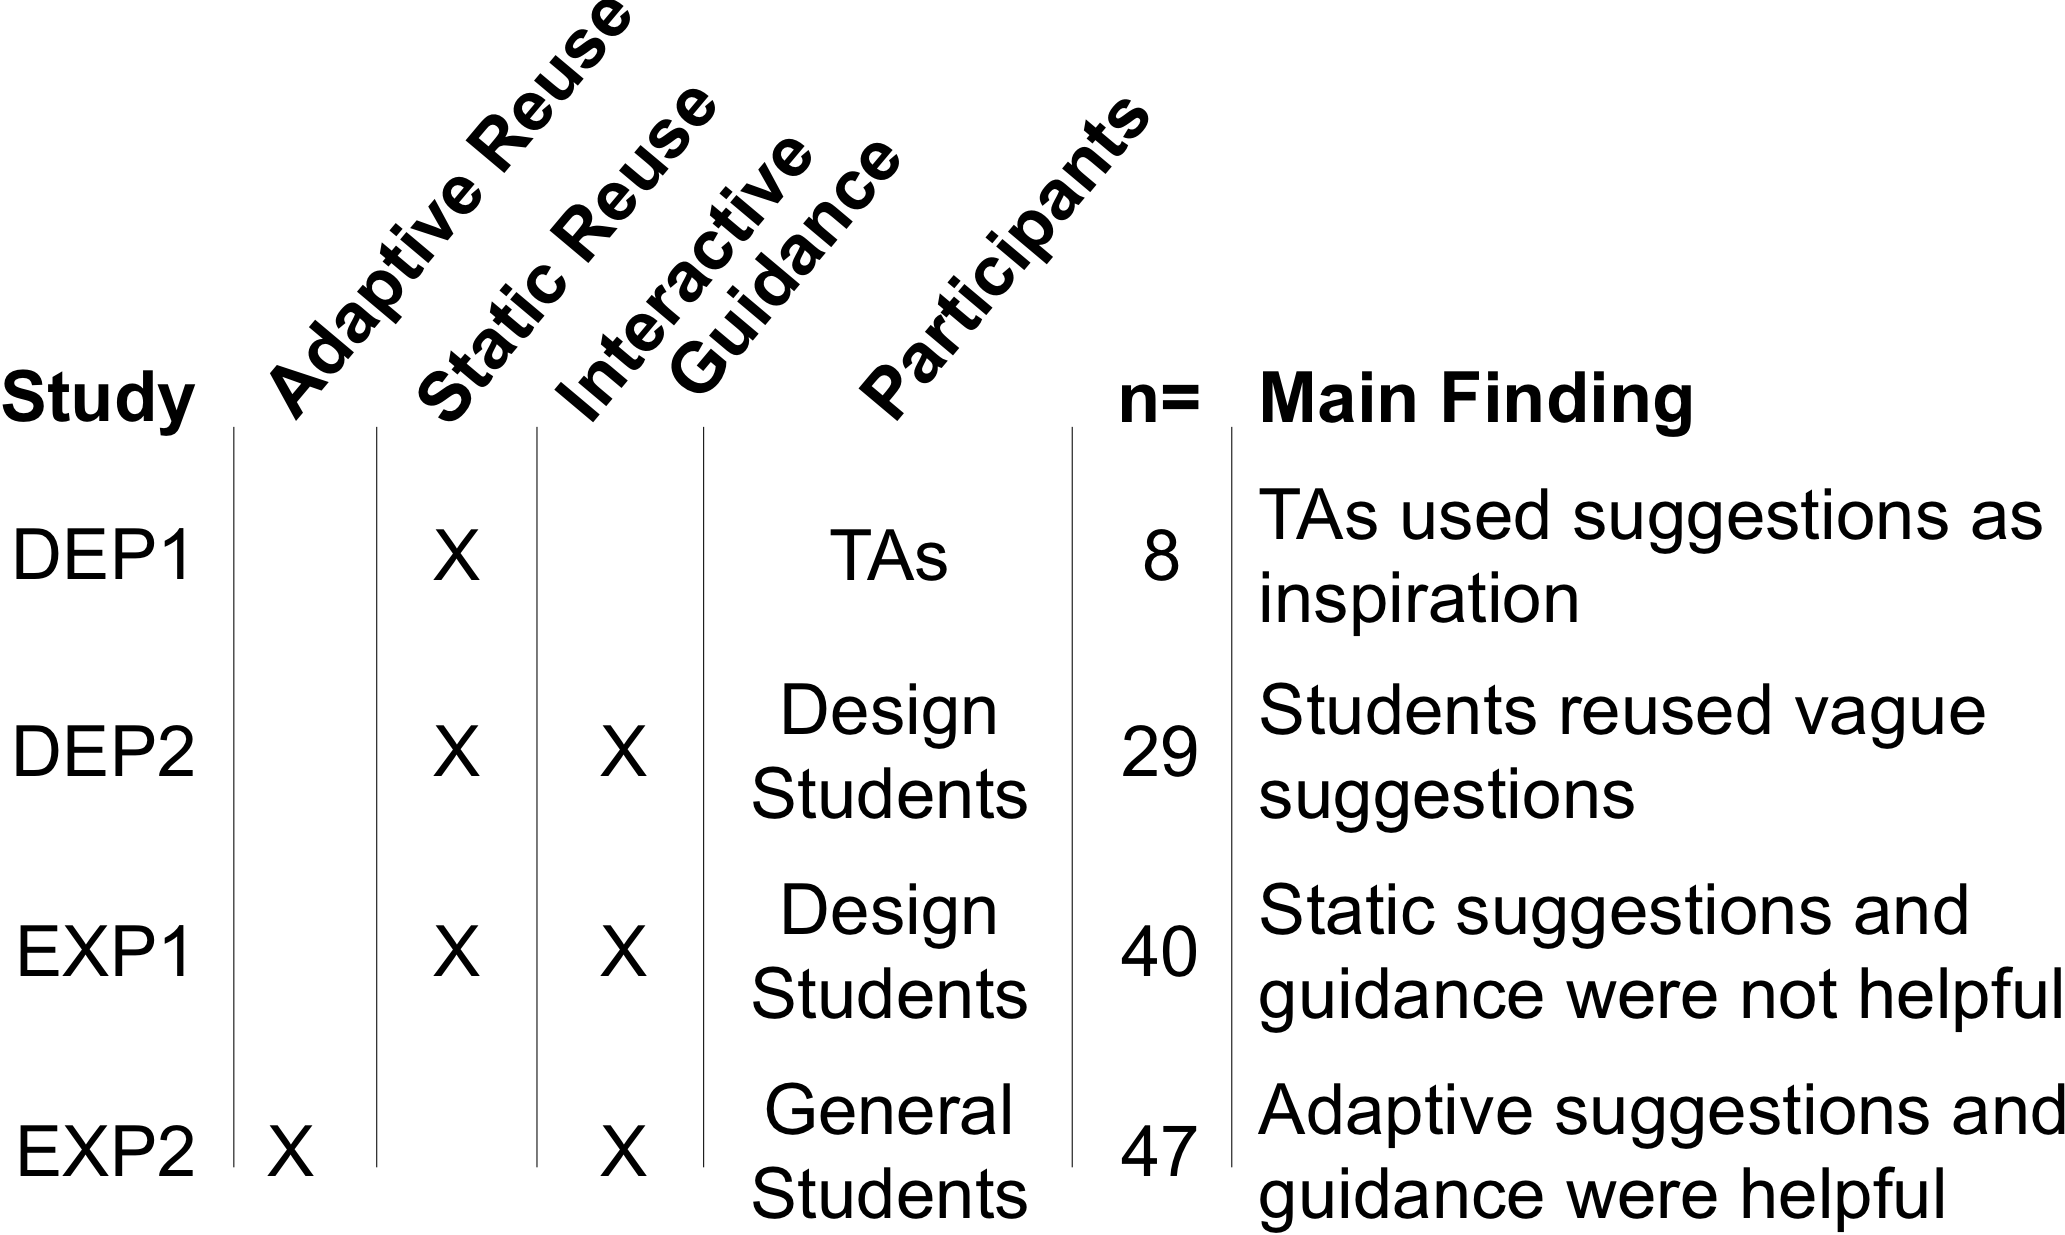
\includegraphics[width=0.6\textwidth]{critiquekit/figures/table1.png}
\end{table}



\section{Related Work}
\subsection{Good Feedback is Actionable, yet Rare}
Rapid iteration is critical to the success of creative projects, from essays, to visual design, to buildings \cite{Dow2010, sadler1989formative}. Receiving feedback early on is important for learners to test alternatives and course-correct \cite{Dow2010, tohidi2006getting}. Effective feedback is especially important in educational settings where novices are learning new skills and developing expertise. However, giving effective feedback is rarely taught \cite{Nicol2006}. As physical and digital classrooms increase in size, the demand for feedback outgrows the ability to adopt the ideal learning model of one-to-one feedback \cite{bloom1984}. Instead, a one-to-many approach is utilized, where an expert provides feedback for multiple learners. Although learners most value expert feedback \cite{Gielen2010, Yang2006}, the one-to-many approach is highly demanding on experts, and effective feedback for individuals becomes increasingly rare. 

In general, effective feedback is specific, actionable, and justified. Specific feedback is direct and related to a particular part of the work rather than vaguely referent \cite{Krause2017, sadler1989formative, yuan2016}. Specific positive feedback also highlights strengths of the work and provides encouragement, so the recipient can tell they are on a good path \cite{Kelley2013, Tseng2007, yuan2016}. Actionable feedback is important because it offers the learner a concrete step forward \cite{sadler1989formative, sommers1980revision, Tseng2007, yuan2016}. Simply pointing out a problem is not sufficient to help one improve \cite{Ramaprasad1983, sadler1989formative, sommers1980revision, tohidi2006getting}. Actionable feedback is often most helpful early in a project \cite{Cho2006, Tseng2007, yuan2016} because it may help people self-reflect and self-evaluate their work \cite{Gibbs}, prompting more revisions for improvement \cite{Dow2012, Topping1998}. Lastly, justification is an important characteristic of feedback \cite{Krause2017, Narciss2006, yuan2016}, but is arguably one of the hardest to understand or recognize \cite{Gielen2010}. Justified feedback contains an explanation or reason for a suggested change, which helps the learner understand why the feedback was given.

\subsection{Rubrics \& Examples Usefully Focus Feedback}
Rubrics \cite{andrade2005teaching, yuan2016} and comparative examples \cite{Krause2017} are effective in structuring feedback because they beneficially encourage attention to deep and diverse criteria. Novices otherwise tend to focus on the first thing they notice, often surface-level details \cite{Greenberg2015, hicks2016framing, Kulkarni2015, yuan2016}. Viewing examples of past designs can lead to greater creativity and insights \cite{kulkarni2012early, marsh1996examples}; thus, showing examples of good feedback may spark ideas reviewers would not have otherwise considered \cite{Greenberg2015, kulkarni2013peer, Luther2015}. Also, adaptive examples curated to match design features are more helpful than random examples in improving creative work \cite{Lee2010}. 

Rubrics and other scaffolds require significant upfront manual work by experts who must carefully design a comprehensive rubric, curate a thorough set of examples, or decide how else to structure the feedback process. This chapter investigates leveraging existing feedback to dynamically create rubric criteria. We hypothesize that showing reviewers previously-provided feedback can guide their attention to important aspects of the design. 

\subsection{Is Feedback Too Context-specific for Practical Reuse?}
Schön persuasively argues that effective feedback should be context-specific and expert-generated \cite{schon1984reflective}. He offers a vignette from architecture where the teacher suggests an alternative building to the student as an example of situated wisdom and its transfer. If Sch\"{o}n is right that this exchange requires both wisdom and context, does that mean that feedback reuse is infeasible? Within a given setting, project, or genre, common issues recur. Hewing to the principle of recognition over recall, we hypothesize that suggestions and guidance can increase novices' participation in context-specific exchanges. 

\subsection{Prior Systems \& Approaches for Scaling Feedback}
Existing approaches for scaling personalized feedback include clustering by similarity (\textit{e.g.}, for writing \cite{Brooks2014} and programming \cite{Glassman2015, Head2017}). Gradescope \cite{Gradescope} and Turnitin \cite{Turnitin} allow graders to create reusable rubric items and comments to address common issues and apply them across multiple assignments. Gradescope binds rubric items to scores, which emphasizes grades rather than improvement. 

Other methods include automating the reuse of the solutions of previous learners. These methods work best when correct and incorrect solutions are clearly distinct, such as in programming \cite{Glassman2016, Hartmann2010} and logical deductions \cite{Fast2013}. Automated methods have also found success with the formal aspects of more open-ended domains such as writing \cite{Brooks2014, Roscoe2014}.  However, assessing the quality and effectiveness of creative work – the strength of a design, the power of a poem – is intrinsically abstract and subjective and lies beyond current automated analysis techniques. Also, little automated analysis exists for media other than text. For domains like design, human-in-the-loop analysis will remain important for quite some time. 

\subsection{Automatically Detecting Feedback Characteristics}
Although feedback is often specific and contextual \cite{schon1984reflective}, general characteristics can be automatically detected and used to help reviewers improve their feedback. For example, PeerStudio \cite{Kulkarni2015} detects when comments can be improved based on the length of the comment and the number of relevant words. Data mining and natural-language processing techniques can also automatically detect whether a comment is actionable or not, and prompt the reviewer to include a solution \cite{Nguyen2016, Xiong2012}. Krause \textit{et al.} use a natural-language processing model to detect linguistic characteristics of feedback and suggest examples to reviewers to help them improve their comment \cite{Krause2017}. These methods require a reviewer to first submit their comment so it can be analyzed, and then improve their comment after submission.

\section{CritiqueKit: Interactively Guiding Feedback}
Based on these methods and insights, CritiqueKit (Figure \ref{fig:critiquekit_interface}) categorizes feedback and provides prompts and suggestions to reviewers. It differs from prior work by providing feedback to reviewers as they type rather than after they submit. We hypothesize that this contextual assistance may provide a just-in-time scaffold that changes how reviewers' thoughts crystallize, yielding feedback that is more specific, actionable, and/or justified. 

Much like the previous systems in this dissertation, CritiqueKit's interface embeds assistance in the context of the user's task, by displaying interactive guidance and suggestions in a panel next to the work being reviewed. Like DiscoverySpace, CritiqueKit prioritizes ease of use for achieving outcomes; users can reuse a feedback suggestion by simply clicking on it. However, unlike DiscoverySpace, CritiqueKit also helps users improve the feedback they come up with from scratch. As our deployments will show, reviewers are often reluctant to directly reuse feedback suggestions, preferring instead to write their own ideas. While DiscoverySpace does not provide support for users who choose to use Photoshop's tools directly, CritiqueKit explores how simple guidance might help reviewers go beyond direct reuse while still achieving outcomes quickly and easily.

\begin{figure}[b!]
\centering
  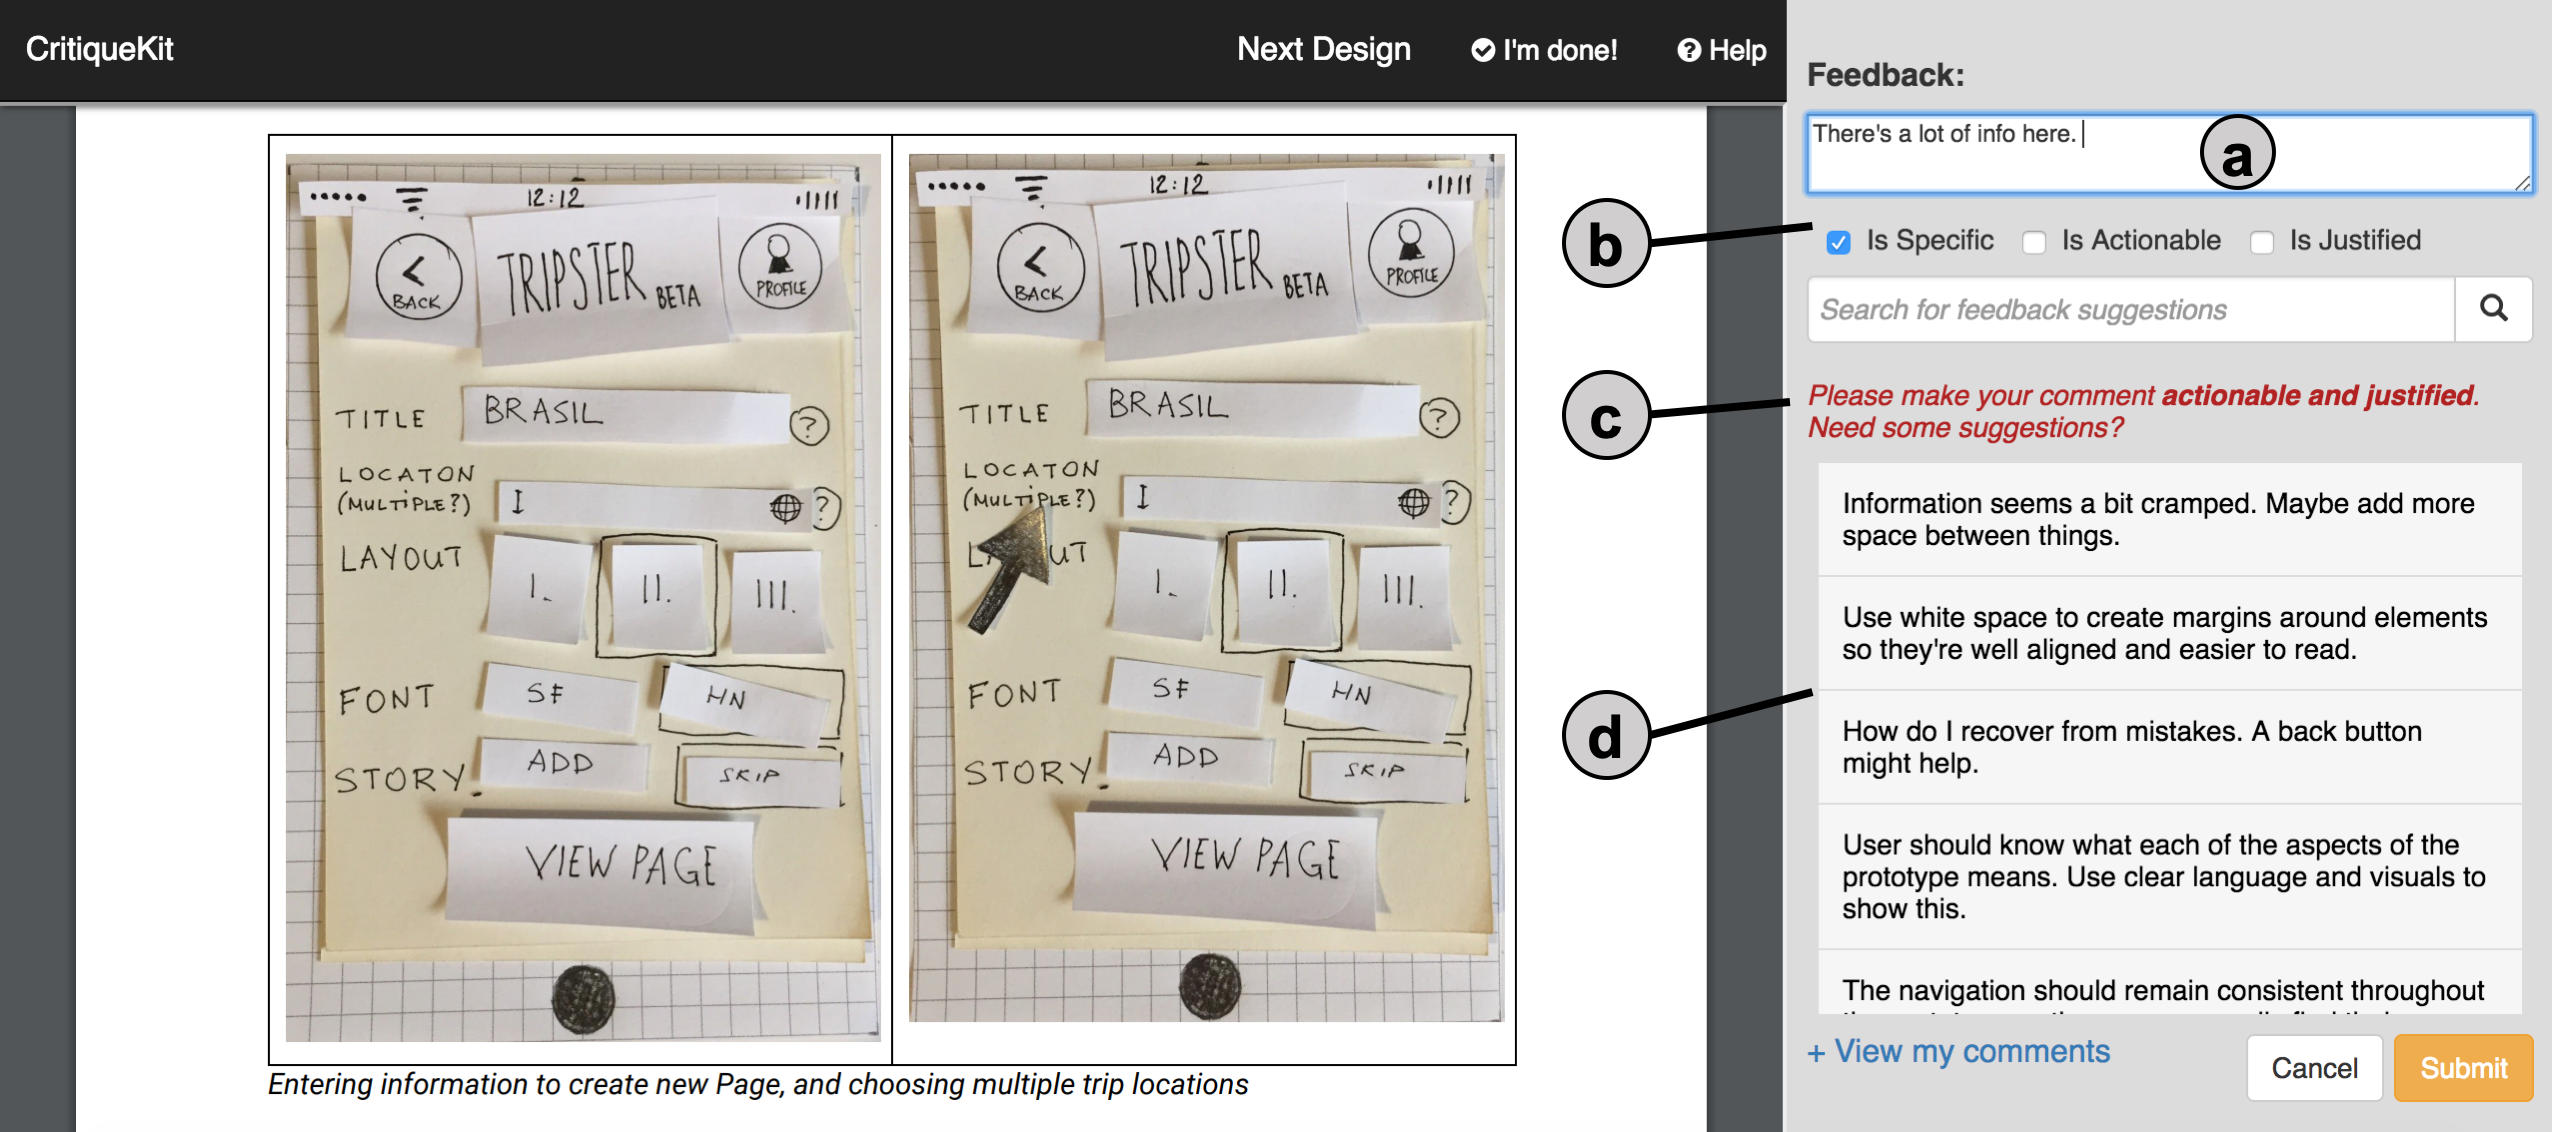
\includegraphics[width=\textwidth]{critiquekit/figures/interface.png}
  \caption[The final CritiqueKit interface (used for Experiment 2).]{The final CritiqueKit interface (used for Experiment 2). a) The reviewer can type their feedback in the textbox. b) The checkboxes in the guidance panel update based on the characteristics of the reviewer’s comments. c) CritiqueKit explicitly prompts reviewers to ensure their comment fits the checkboxes in the guidance panel. d) The reusable feedback suggestions in the suggestions box update based on the unchecked characteristics in the guidance panel, adapting specifically to the reviewer's feedback.}~\label{fig:critiquekit_interface}
\end{figure}

\subsection{Interactive Guidance as a Form of Scaffolding}
CritiqueKit features an interactive guidance panel (Figure \ref{fig:critiquekit_interface}b) with checkboxes that update based on which of three attribute categories the feedback fits: \textit{Is Specific} \cite{Krause2017, sadler1989formative, sommers1980revision, yuan2016}, \textit{Is Actionable} \cite{Dow2012, Gibbs, Kulkarni2015, Luther2015, sadler1989formative, Tseng2007}, and \textit{Is Justified} \cite{Gielen2010, Krause2017, Narciss2006, yuan2016}. 

The prototype assesses the feedback's fit with the following heuristics. The heuristic for the \textit{specific} category merely requires that comments be at least five words long because vague comments tend to be short, such as ``good job'' or ``needs work.'' Perhaps surprisingly, we observed that the five-word nudge was sufficient to garner specific feedback in practice. (Some websites, like Etsy, also use a five-word minimum heuristic for reviews). For the \textit{actionable} and \textit{justified} categories, we manually combed feedback that had been hand-labeled as meeting these categories and observed that specific keywords (i.e., ``maybe try'' and ``you should'' for actionable; ``because'' and ``so that'' for justified) were strong cues of these categories. Consequently, the prototype implementation simply checks for the presence of these keywords and phrases in feedback comments. 

A comment is considered complete once all checkboxes are checked. Reviewers can manually check and uncheck the checkboxes if they feel the checkboxes did or did not add a category in error. For example, if a reviewer's comment states, ``Use a 2-column grid layout,'' and the ``Is Actionable'' checkbox remains unchecked, the reviewer can manually check the checkbox to note that their comment does indeed contain an actionable suggestion. 

\subsection{Adaptive Suggestions for Greater Specificity}
The suggestions box (Figure \ref{fig:critiquekit_interface}d) contains a list of previously given feedback from experts. These suggestions dynamically adapt based on how the reviewer's feedback is categorized in the guidance panel. For example, if a reviewer's comment does not yet satisfy the actionable and justified categories (as in Figure \ref{fig:critiquekit_interface}), the suggestions box would contain examples of feedback with these characteristics. Suggestions appear in the order they were added to the corpus.

\subsection{The CritiqueKit Review Workflow}
When a reviewer first opens CritiqueKit, a prompt asks them to provide specific feedback on something they like about the design and something that could be improved. The suggestions box contains general feedback snippets \cite{kulkarni2013peer} pertinent to the review criteria to give reviewers a starting point, providing suggestions that are broadly applicable and fit within the specified criteria. The ``Submit'' button at the bottom of the interface is red to indicate that the comment text box is either empty or does not fit any of the categories in the guidance panel. 

Once a comment is sufficiently long, the ``Is Specific'' checkbox will check, and the reviewer will be prompted to make their comment actionable and justified. The ``Submit'' button turns yellow to indicate that their feedback is not yet complete, though they can still submit if desired. The feedback suggestions then change to present comments that instantiate both actionable and justified feedback. The suggestions continue to adapt depending on the characteristics of the comment, showing reusable examples of feedback that satisfy the unchecked categories in the guidance panel. The reviewer can insert a suggestion directly into their own feedback by clicking on it. They can then edit the suggestion if they wish in the text field. Once all checkboxes are checked, the ``Submit'' button turns green as an indication of completeness. 

Using prior feedback as suggestions can give inspiration and highlight common issues. The presence of the structured guidance panel reminds reviewers of attributes that feedback should have. 

\subsection{Implementation}
CritiqueKit is a client-server web application implemented using Node.js; it assumes that all content to be reviewed is available on the web. The corpus of reusable feedback comments is stored on the server in \textsc{json} format.

CritiqueKit uses web sockets for communication between each client running the application and the main server, implemented using the socket.io module. Feedback classification happens on the client-side using JavaScript. Feedback suggestions are also generated on the client-side after retrieving the corpus from the server; the suggestions box adaptively shows and hides comments using JavaScript. 

Users access CritiqueKit by navigating to its \textsc{url} in a web browser. The first time the browser loads the website, a unique \textsc{id} is generated for the user and sent to the server. A cookie is also saved on the client-side so that the server can identify and differentiate users. The review content is loaded within the page as an iframe.

\section{Deployments: (How) Is Feedback Reused?}
To understand how feedback is reused in educational settings and evaluate the CritiqueKit approach, we conducted two deployments and two experiments. All studies took place at a research university. 

\subsection{Deployment 1: How Do Teaching Assistants Reuse Feedback?}
Eight teaching assistants (TAs) (two female) for an undergraduate design course used Gradescope to grade and critique seven weekly assignments that varied in content from storyboards to written explanations to high-fidelity web application prototypes. TAs set rubric items for each assignment and wrote comments for each. We deployed CritiqueKit to first understand how TAs might reuse feedback and made iterative improvements to the design throughout the quarter based on TA input.

\begin{figure}[b!]
\centering
  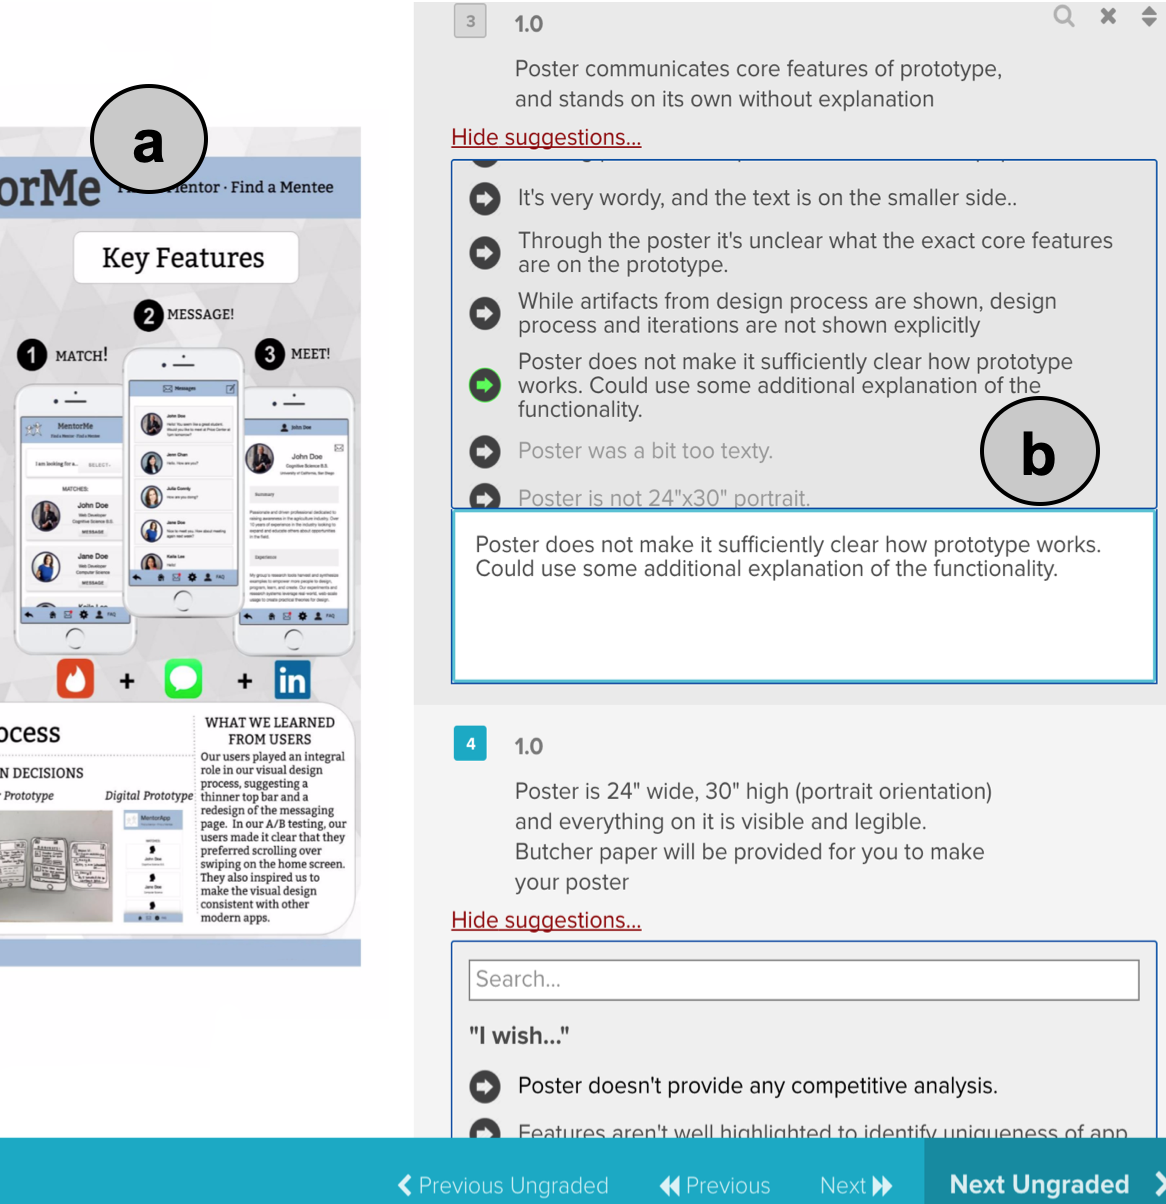
\includegraphics[width=0.6\textwidth]{critiquekit/figures/gradescope.png}
  \caption{CritiqueKit implemented as a browser extension in Gradescope for Deployment 1. a) Reviewers provide feedback on a student design. b) The suggestions box under each rubric item provides reviewers with a list of reusable suggestions and a comment box for providing feedback on a submission.}~\label{fig:critiquekit_gradescope}
\end{figure}

\subsubsection{Method: Integrating CritiqueKit with Gradescope}
To integrate with the TAs' existing workflow, we implemented CritiqueKit as a Google Chrome extension that augments the Gradescope interface with a suggestions box (Figure \ref{fig:critiquekit_gradescope}). This version of CritiqueKit contained only the suggestions box to explore feedback reuse. The suggestions box contained a manually curated set of feedback provided by former TAs in a previous iteration of the course, stored in a Google Sheet online and retrieved by the Chrome extension using the Google Sheets \textsc{api}. Suggestions were categorized into three feedback categories: Positive, Problem, and Solution. TAs could select feedback suggestions to directly copy into the textbox for further editing. Each rubric item contained its own suggestion box interface, providing suggestions specific to that rubric item.

We curated the reusable suggestions corpus as follows. Given all feedback from the previous quarter, feedback that was 25 or fewer words in length was kept, because longer feedback was both too long to be skimmed in a suggestion display and tended to be overly specific. Feedback of 26-30 words was truncated at the sentence level to fit within the 25-word limit. Longer comments or duplicate comments were discarded. In total, 526 comments were provided as suggestions throughout the course for seven (of ten) assignments. Suggestions were manually categorized into the Positive ($n = 92$), Problem ($n = 312$), and Solution ($n = 122$) categories.

\subsubsection{Result: TAs Used Feedback Suggestions as Inspiration}
Across seven assignments, four of the eight TAs reused 51 distinct suggestions from the 526-element corpus (9.7\%). 75 of 583 designs received a reused suggestion for feedback. 60\% of reused suggestions were categorized in the Problem category. These numbers omit any reuse occurring entirely inside Gradescope without CritiqueKit. (Gradescope provides an interface for reusing entire comments within an assignment rather than for individual parts of the comment.) 

An end-of-course survey asked TAs about their CritiqueKit use. One commented that he would ``\textit{skim the comments in the [suggestions] to see if something was accurate to my thoughts}.'' Another mentioned that the prototype helped him ``\textit{[find] ways to better explain and give feedback about specific points}.'' TAs also mentioned that suggestions sometimes reminded them to comment on more diverse aspects of students' work. For example, one mentioned that seeing positive suggestions reminded her to give positive feedback, not only critiquing areas for improvement. TAs mentioned using the suggestions as inspiration rather than the exact wording, taking the underlying concept of a suggestion and tailoring it.

\subsection{Deployment 2: How Do Students Reuse Feedback?}
The first deployment examined teaching staff usage; this second deployment examined student usage to understand how novices interact with guidance and suggestions. We deployed CritiqueKit as a standalone web application with 29 students in an undergraduate design course for five weeks. Students gave anonymous feedback on two randomly assigned peer submissions for each of seven assignments.

\begin{figure}[b!]
\centering
  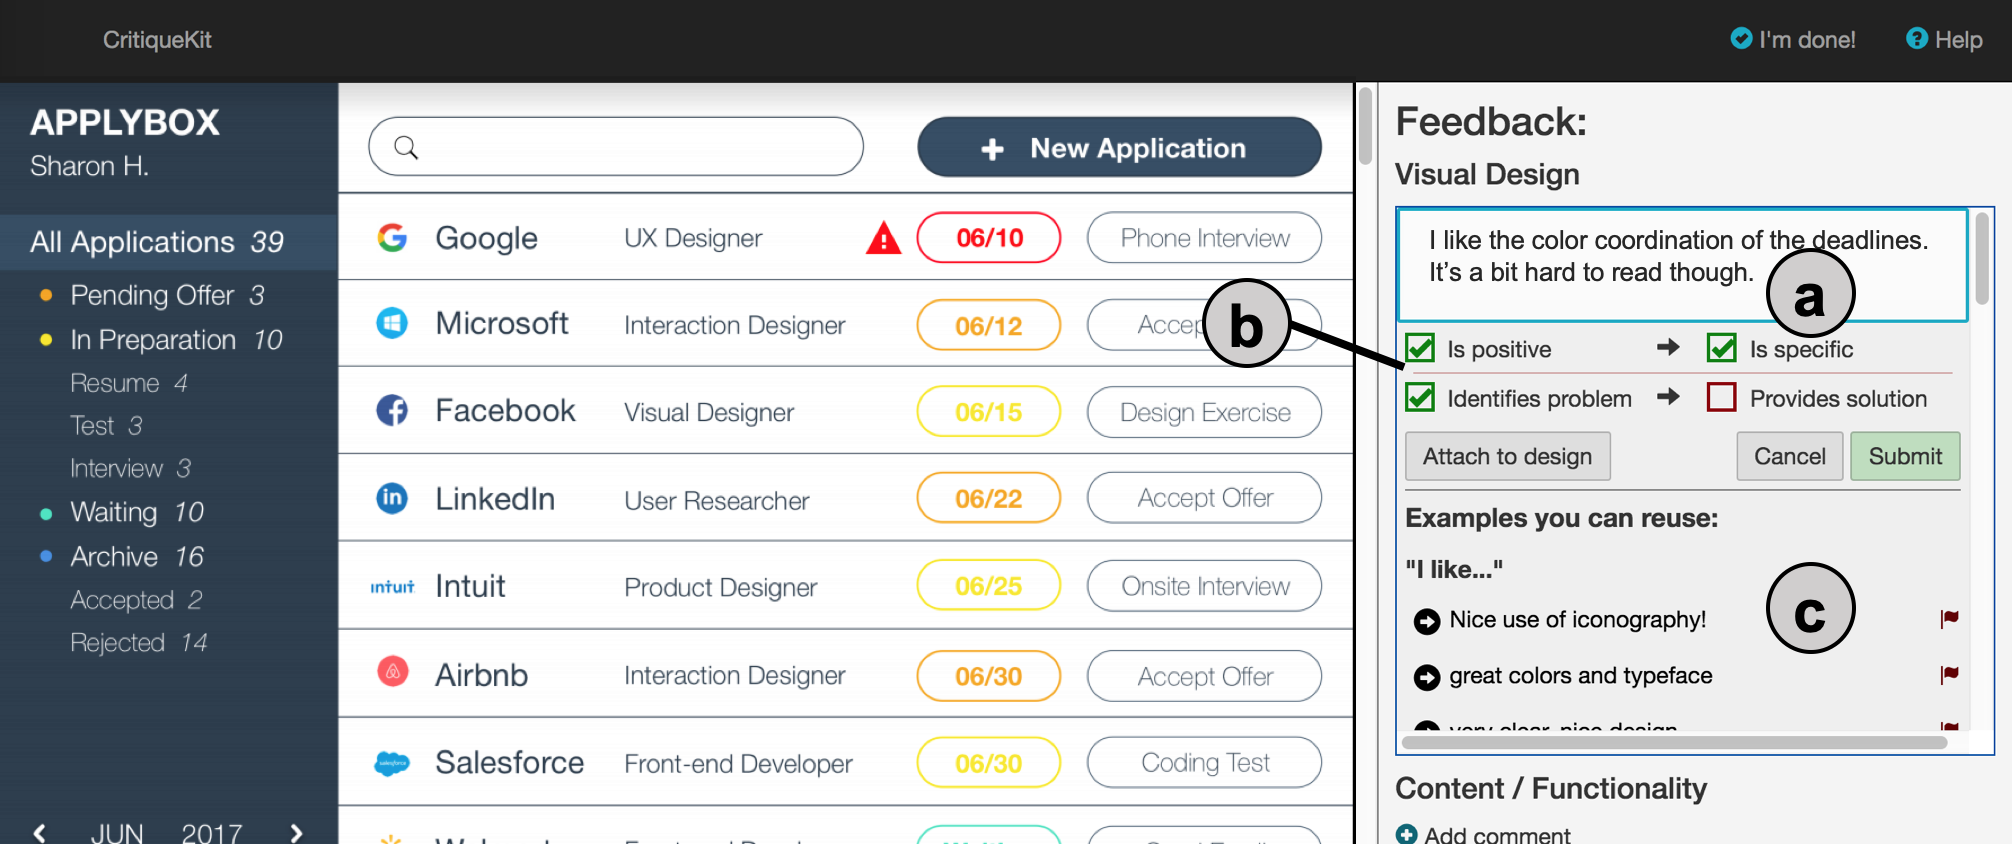
\includegraphics[width=\textwidth]{critiquekit/figures/old_interface.png}
  \caption[The CritiqueKit user interface for Deployment 2 and Experiment 1.]{The CritiqueKit user interface for Deployment 2 and Experiment 1. a) The reviewer types their feedback into the text box. b) Checkboxes in the guidance panel update as the reviewer types to show how well the comment fulfills high-quality feedback criteria. c) The reviewer can browse and reuse previously given feedback.}~\label{fig:critiquekit_exp1}
\end{figure}

\subsubsection{Method: Integrating Interactive Guidance for Scaffolding}
Novice students are less experienced in giving feedback and may benefit from interactive scaffolding \cite{Reiser}. This version of CritiqueKit included an interactive guidance panel to help reviewers provide more specific and actionable feedback (Figure \ref{fig:critiquekit_exp1}). The categories on the guidance panel were ``Is Positive,'' ``Is Specific,'' ``Identifies a Problem,'' and ``Presents a Solution'' with checkboxes next to each. These categories stem from recommendations in the literature for both positive and critical feedback \cite{Kelley2013}. Similar to the final version of CritiqueKit, these checkboxes updated as a reviewer typed by classifying their comment into the three categories. The categories differed from the final version, focusing on specific and actionable feedback. 

The suggestions box was seeded with feedback from the course TA. Similar to the first deployment, the suggestions were categorized in the Positive, Problem, and Solution categories. When a student submitted a comment, it was classified into one of these categories, shortened to 25 words if it was longer, and fed back into the corpus to appear as a suggestion, enabling students to reuse their peers' as well as their own comments. The suggestions were ordered first by frequency used, then by shortest length first, and updated as these values changed and more comments were added. Compared to the final version of CritiqueKit, suggestions were static, meaning they did not change as the reviewer typed.

\subsubsection{Results: Positive Feedback Common; Reuse Rare}
For seven assignments, 898 comments were submitted. Independent raters classified each comment into the five categories of Positive Only, Positive  and  Specific (Positive + Specific), Problem Only, Solution Only, and Problem with a Solution (Problem + Solution). 45\% of these comments contained positive feedback; 30\% contained a Problem + Solution statement. 

Students rarely selected feedback suggestions for reuse. Over the five-week deployment, 14 distinct suggestions were reused on 27 student designs for four of the seven assignments. These suggestions were mostly short, vague comments such as ``I wish this was more visually appealing.'' This may be because students often left feedback specific to individual designs that did not easily generalize to other contexts. Students' comments in a post-survey confirmed that the suggestions did not always seem applicable. Students also did not regularly use the interactive guidance panel; 15 of the 29 students engaged with the panel a total of 120 times over five weeks. 

In contrast to how TAs reused feedback, students may not have recognized common issues. TAs paid attention to common errors between designs and mainly reused Problem feedback, whereas students may not have noticed or attended to underlying issues between designs. For instance, one student mentioned that they did not use the feedback suggestions because they ``\textit{rarely pointed out the same things when critiquing interfaces}.'' 

This exploratory deployment investigated how students reuse feedback and respond to interactive guidance in the classroom. To understand how a system with these features compares to a standard feedback system, the next study was a controlled between-subjects experiment. 

\section{Experiments: Scaffolding Feedback}
\label{sec:critiquekit_exp}
Following our deployments, we conducted two empirical studies to investigate the impact of suggestions and guidance on feedback quality.

\subsection{Experiment 1: Do Static Suggestions Improve Feedback?}
In an online between-subjects study, 40 undergraduate design students were asked to review three restaurant website homepages using CritiqueKit. The task emulated peer review tasks often required in creative courses. This study's suggestion corpus came from a design feedback task on CrowdCrit \cite{Luther2015} and was categorized in the Positive, Problem, and Solution categories. We hypothesized that suggestions and guidance would help reviewers provide more specific and actionable comments.

\subsubsection{Method: Reviewing Restaurant Websites}
40 participants were randomly assigned to either the CritiqueKit condition or the Control condition (20 in each). CritiqueKit participants used the same version of CritiqueKit as Deployment 2 with all features available (Figure \ref{fig:critiquekit_exp1}). Control participants used an otherwise identical version consisting solely of a comment text box. Upon landing on the homepage of either version, participants were provided with a scenario explaining that three restaurant owners are seeking feedback on their new website design. Participants were given a brief tutorial of CritiqueKit's features and an explanation of what makes for good feedback. There were no restrictions or requirements on time spent or amount of feedback to provide. We compared the percentages of comments in five categories. Comments including a supportive element were labeled as \textit{Positive Only} or \textit{Positive + Specific}. Comments including a critical element were labeled \textit{Problem Only}, \textit{Solution Only}, or \textit{Problem + Solution}.

\begin{figure}[b!]
\centering
  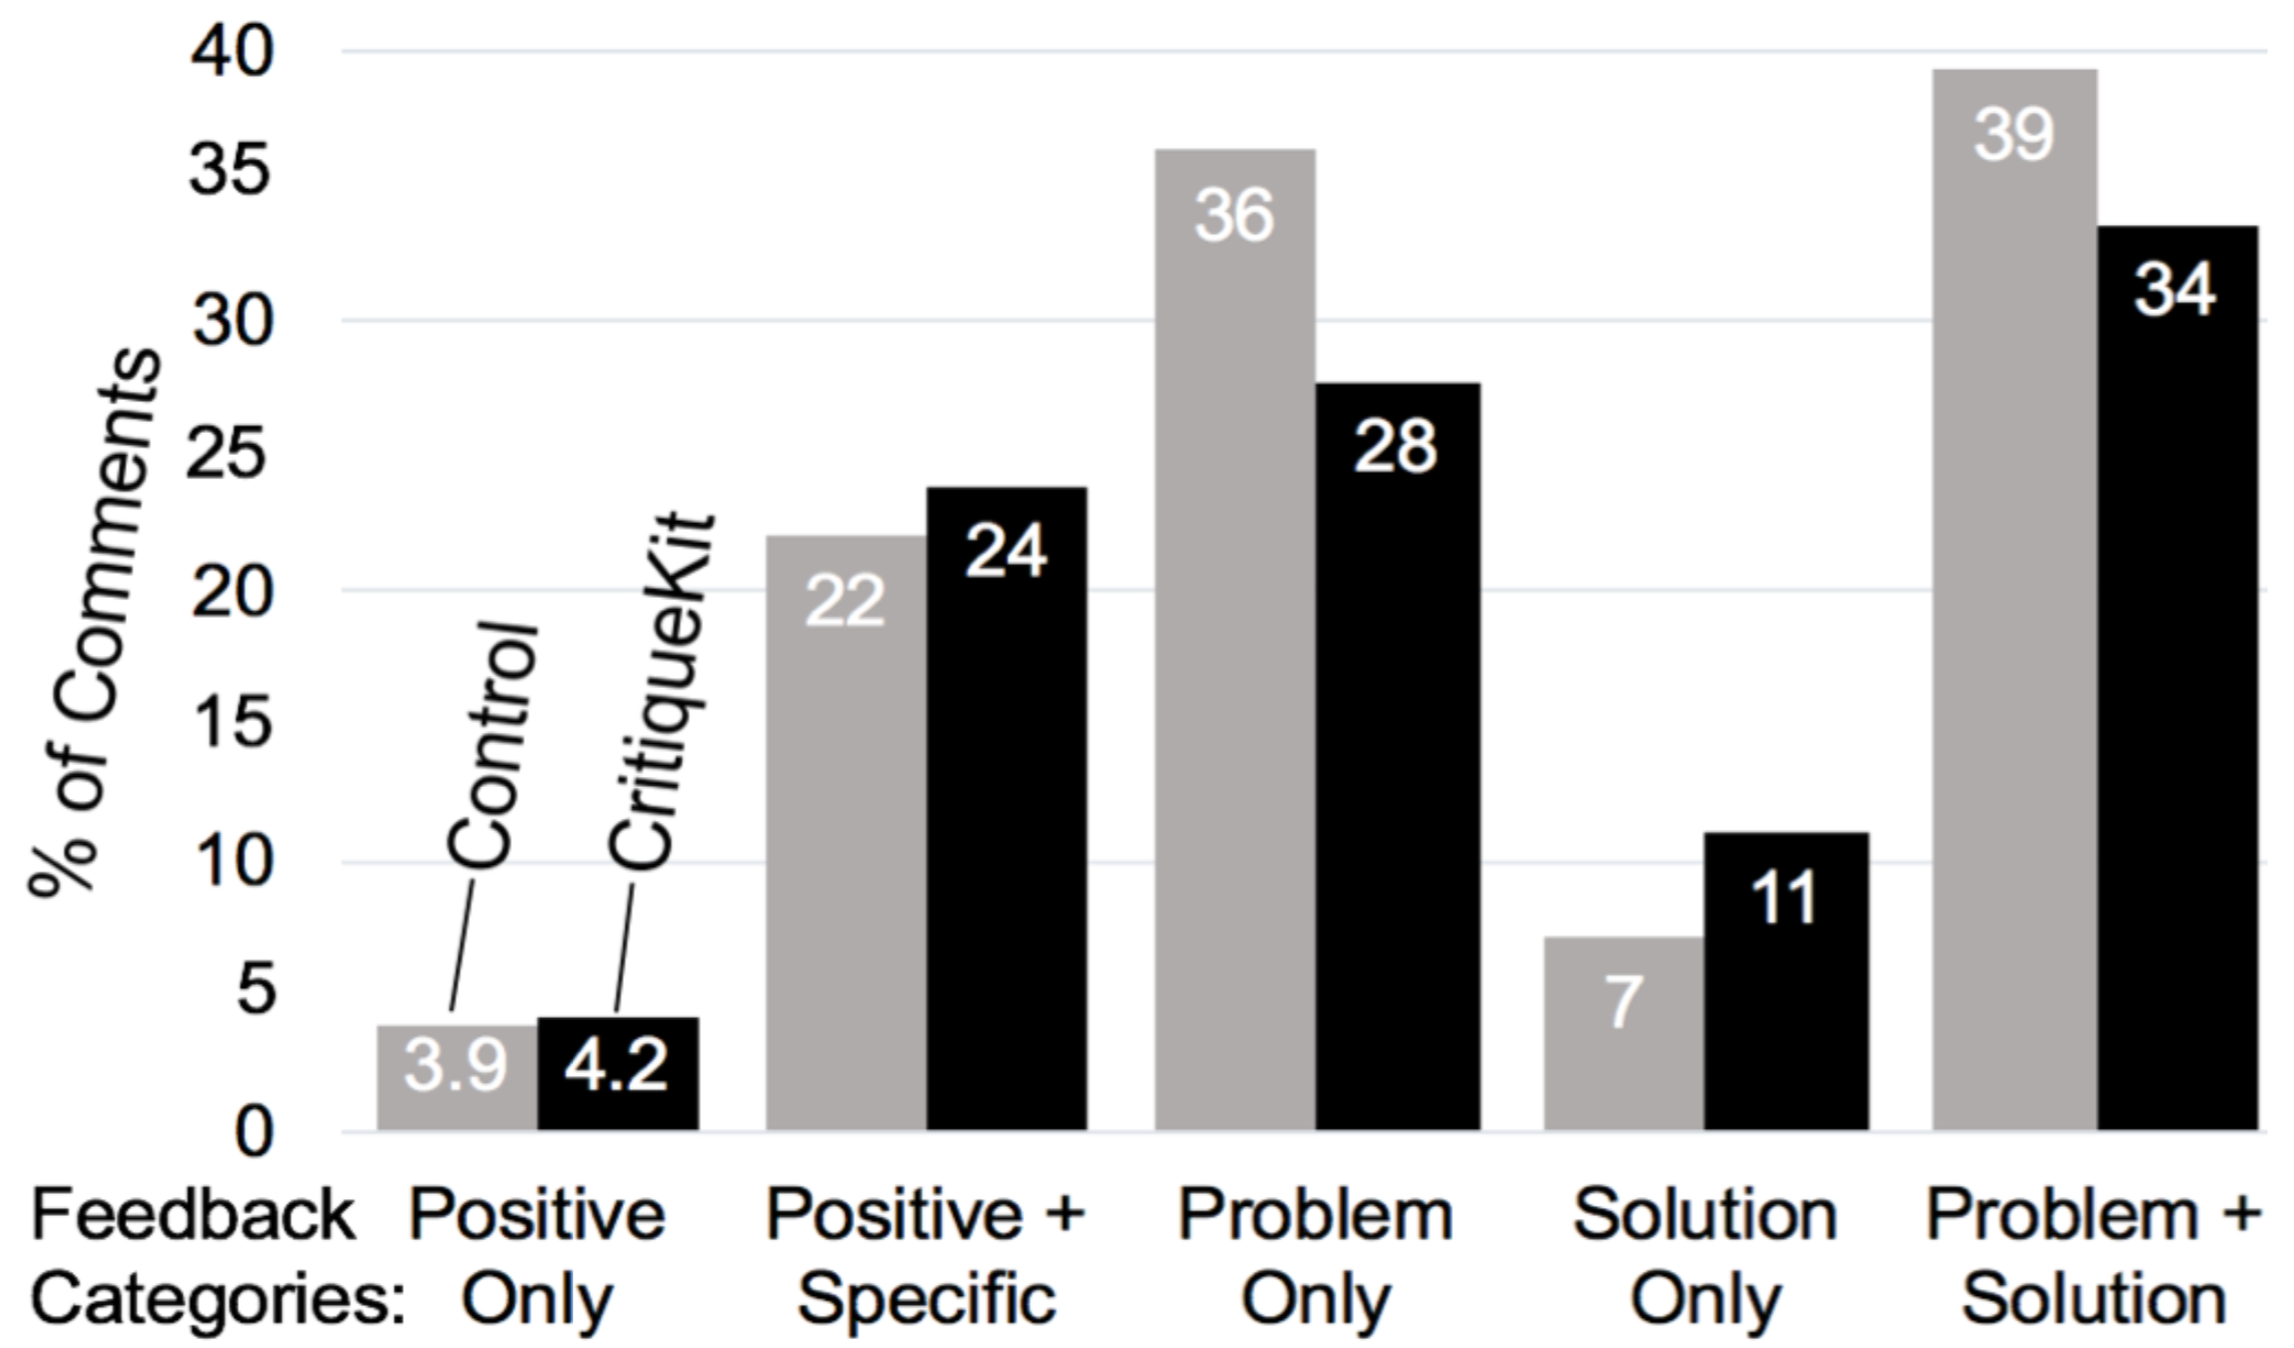
\includegraphics[width=0.8\textwidth]{critiquekit/figures/exp1_feedbacktypes.png}
  \caption{A plurality of feedback in both conditions in Experiment 1 identified both a problem and solution (\textit{i.e.}, was actionable). Feedback that was only positive was the rarest. There were no significant differences between conditions for these categories.}~\label{fig:critiquekit_exp1_results}
\end{figure}

\subsubsection{Results: Static Suggestions Were Not Helpful}
With static suggestions and interactive guidance, there were no significant differences between conditions. (To foreshadow, we will see differences in Experiment 2, which adds adaptive suggestions). Participants provided a total of 323 comments (168 for control, 155 for CritiqueKit). The average number of words per comment was not significantly different between conditions (Control: $m = 29.07, SD = 23.64$; CritiqueKit: $m = 23.22, SD = 17.3$) ($F(1,38) = 2.52, p = .11$).

\subsubsection{Suggestions \& Guidance Did Not Affect Type of Feedback}
The distribution of the five category types did not vary significantly between conditions ($x^2 = 4.80, df = 4, p = .31$) (Figure \ref{fig:critiquekit_exp1_results}). In both groups, participants provided mostly Problem + Solution feedback (39\% in Control; 34\% in CritiqueKit). 

\subsubsection{Most CritiqueKit Participants Corrected Category Labels}
65\% of CritiqueKit participants actively used the guidance panel, making a total of 85 corrections to categories. Interaction with the guidance panel may have indicated attention to the feedback characteristics. As the study was online, we don't know how many of the other 35\% were influenced by the guidance panel. 

\subsubsection{Unfortunately, People also Reused Vague Suggestions}
11 distinct suggestions from the corpus were reused. 8 of these were vague; 3 were specific. 15 of 155 reviews included a reused suggestion. This seems especially low given the high engagement with the guidance panel. We see two reasons for this: First, the suggestions came from CrowdCrit \cite{Luther2015}, where participants provided feedback on a weather app design. The study task was different than the task for which the suggested feedback was originally given, and novices may have had a limited ability to see the deep structure behind a suggestion and reapply it in a new context. Second, the suggestions were created by crowd workers and of uneven quality. 

The suggestions selected were typically short, positive comments, perhaps because students did not know how to apply them in the specific context. For example, the most commonly reused suggestion was ``great use of color'' (reused 3 times). This result is similar to Deployment 2 in which students did not find feedback provided by other peers or novices to be useful and generalizable. Feedback suggestions may require more curation or quality control to be most useful. 

\subsubsection{Suggestions \& Guidance Should Work in Concert}
While this version of CritiqueKit contained both feedback suggestions and interactive guidance, these features functioned independently. Regardless of the categories checked in the guidance panel, the suggestions remained static and presented in the same order for each participant, potentially making them easy to ignore if they were irrelevant to the context. Participants may have paid attention to only one feature at a time. The next study investigated the question of whether adaptively presenting feedback suggestions along with interactive guidance improves feedback. 

\subsection{Experiment 2: Do Adaptive Suggestions Help?}
The second experiment used the final version of CritiqueKit described in the system section to test the hypothesis that adaptively-presented suggestions combined with guidance would improve feedback by increasing the fraction of feedback that is specific, actionable, and/or justified.

\subsubsection{Method: Reviewing Paper Prototypes}
We conducted a between-subjects in-person study with 47 (27 female) participants. Participants were recruited from an undergraduate subject pool within the Psychology and Cognitive Science departments. Participants were randomly assigned to either the CritiqueKit ($n = 24$) or Control ($n = 23$) conditions. 44 of these participants had no design course experience; 3 participants had taken at least one design course. 28 spoke English as a second language. 

Participants were asked to provide feedback on two designs from students enrolled in an online course who volunteered to receive more feedback on their work. These designs were PDFs of mobile application paper prototypes. The review criteria included whether the prototype supported the student's point of view and whether it seemed easily navigable. Participants were first shown the design instructions and review criteria and then given a short tutorial of CritiqueKit as well as an explanation of what makes for good feedback. CritiqueKit participants had all features of CritiqueKit available to them (Figure \ref{fig:critiquekit_interface}), while Control participants used a version that consisted of only a textbox for their feedback. The task took about 30 minutes to complete. After providing feedback on both designs, participants were interviewed about their feedback process and use of CritiqueKit. 

\subsubsection{Presenting Feedback Suggestions Adaptively}
The categories on the guidance panel and their definition used for coding participants' responses were the following:\\
\textbf{Specific}: relates directly to the review criteria\\
\textbf{Actionable}: gives a concrete suggestion for improvement\\
\textbf{Justified}: provides a reason for why something is done well or should be improved

For Deployment 2 and Experiment 1, the guidance panel categories sought to encourage specific and actionable feedback (Figure \ref{fig:critiquekit_exp1}). Examining the feedback from our previous studies, we found that ``Is Positive'' and ``Identifies a Problem'' did not provide significant guidance as reviewers were generally aware of whether their feedback was positive or critical. In addition, the guidance panel did not explicitly check for justification of feedback. For Experiment 2, we revised the categories to ``Is Specific,'' ``Is Actionable,'' and ``Is Justified'' to also encourage the explanation or reasoning behind feedback. As described in the system section, the checkboxes update as the reviewer types to reflect the categories present in their comment, and the suggestions adapt to show feedback examples from categories not yet present in the comment. 

\subsubsection{Results: CritiqueKit Participants Provided a Greater Proportion of Specific, Actionable, \& Justified Feedback}
\begin{figure}[b!]
\centering
  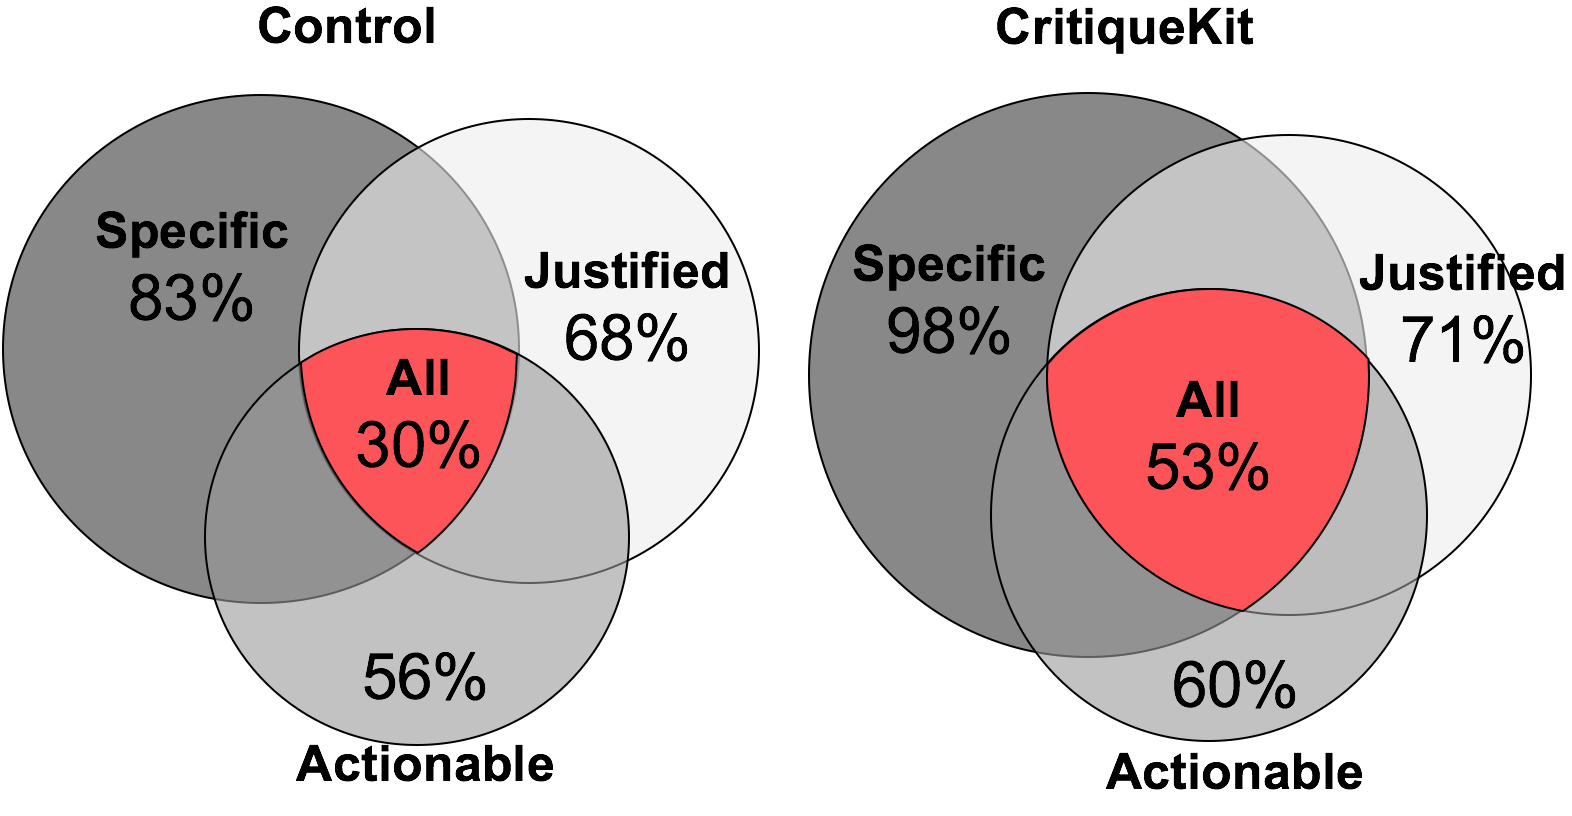
\includegraphics[width=0.7\textwidth]{critiquekit/figures/venn_diagram_exp2.png}
  \caption{In Experiment 2, a significantly higher percentage of feedback in the CritiqueKit condition ($n=24$) (53\% versus 30\%) contained three attributes of good feedback: Specific, Actionable, and Justified ($x^2=8.33, df = 1, p = .01$) than in the Control condition ($n=24$).}~\label{fig:critiquekit_exp2}
\end{figure}

Participants provided 158 total comments (79 control, 79 CritiqueKit). The percentage of comments that contained all three categories (specific, actionable, and justified) was significantly higher in the CritiqueKit condition (53\%) than in Control (30\%) ($x^2=8.33, df = 1, p = .01$) (Figure \ref{fig:critiquekit_exp2}). As an example, this comment meets all three: ``The `more questionnaires' section (Specific) should be made smaller (Actionable) because it is not the main focus of the page.'' (Justified). The system's heuristic for checking specificity of a comment was quite simple: five words or greater in length. Feedback raters blind to each condition used a more sophisticated and holistic assessment, taking specific to also mean related to the review criteria. With this assessment, 98\% of CritiqueKit comments were labeled by raters as specific whereas only 83\% of Control comments were. These raters also rated comments from Experiment 1 within the specific, actionable, and justified categories to provide a comparison between the two experiments. Interestingly, the percentage of comments containing all attributes in the Control condition was relatively consistent between Experiment 1 (35\%) and Experiment 2 (30\%). The percentage of comments with all attributes in the CritiqueKit condition greatly increased between the two experiments (26\% versus 53\%). Having the checkboxes may have explicitly reminded CritiqueKit participants to ensure their comments satisfy the specific, actionable, and justified categories.

\begin{figure}[b!]
\centering
  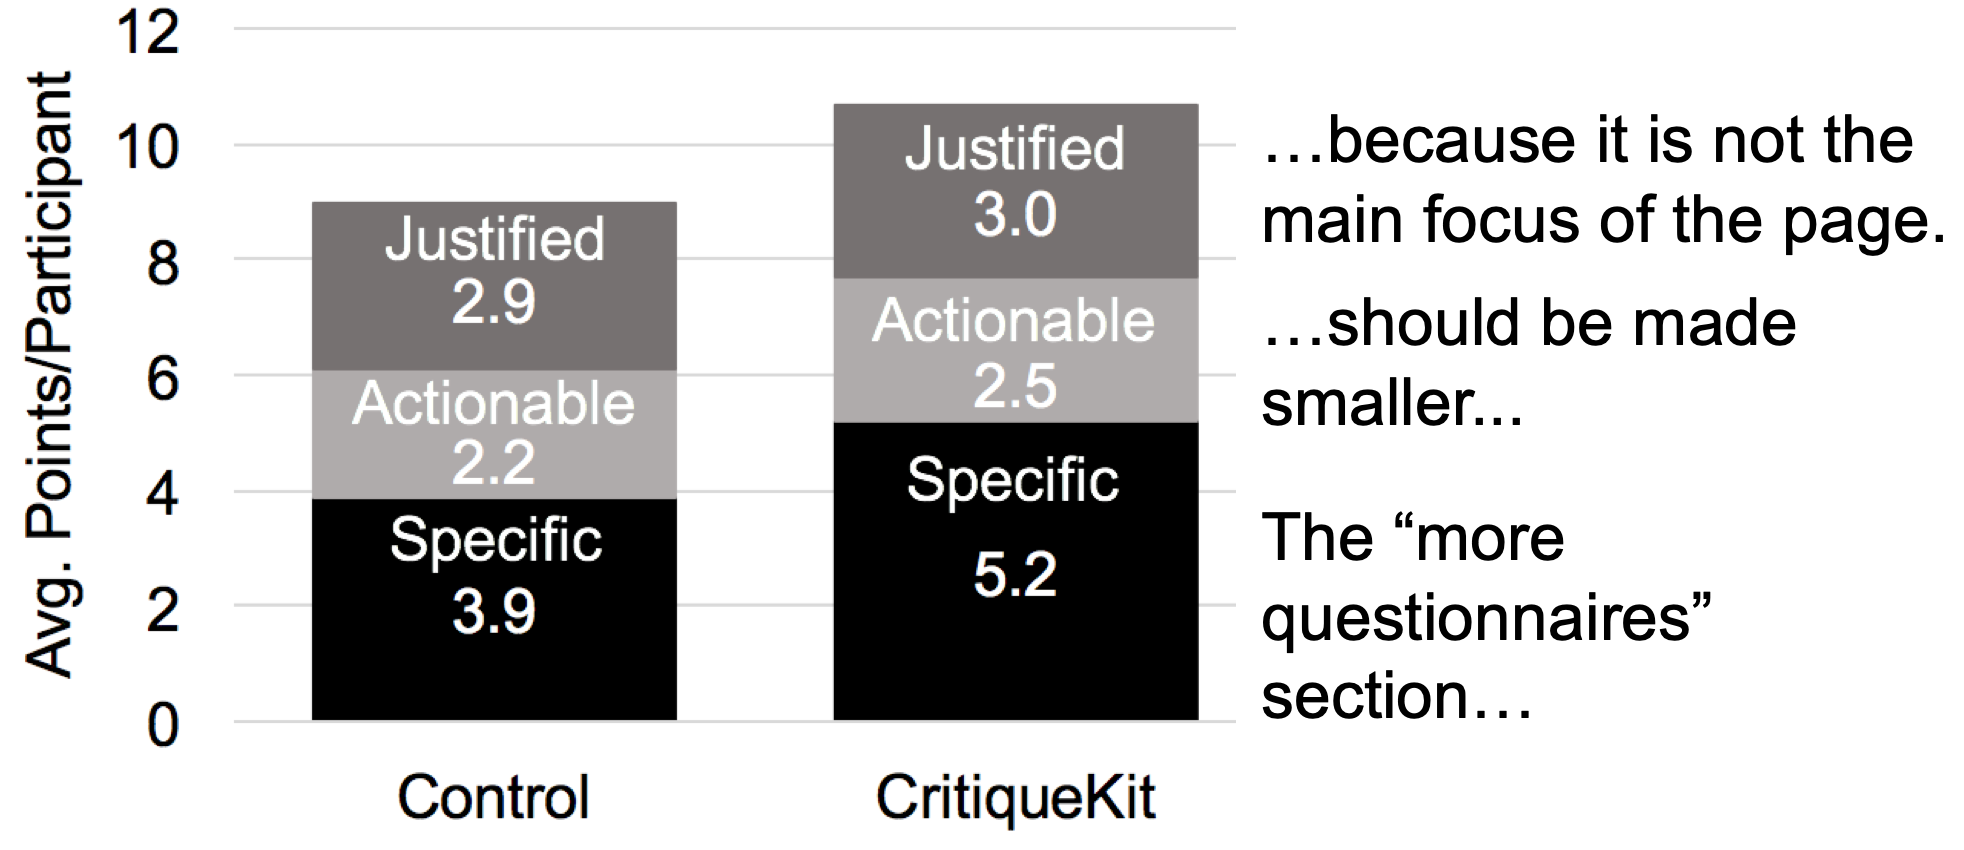
\includegraphics[width=0.8\textwidth]{critiquekit/figures/exp2_bar.png}
  \caption{CritiqueKit participants ($n=24$) provided more \textit{specific} and \textit{all-three} category ideas than Control participants ($n=23$)($F(1,156) = 8.78, p < .005$).}~\label{fig:critiquekit_exp2_bar}
\end{figure}

Because longer comments were more likely to contain all three categories, each comment was also scored on a point scale and averaged per participant. Comments received one point for each specific, actionable, and justified idea (Figure \ref{fig:critiquekit_exp2_bar}). A \textsc{manova} with category points as dependent variables shows a significant difference between conditions ($F(1,3) = 3.21, p < .005$). CritiqueKit participants provided more specific ideas than Control participants (Control $m = 3.87$, CritiqueKit $m = 5.17$, $F(1,156) = 14.04, p  <  .05$). This may be because the suggestions provided examples of relevant ideas and led CritiqueKit participants to address more. CritiqueKit participants also provided more ideas that fit all three categories than control (Control $m = 1.0$, CritiqueKit $m = 2.2$, $F(1,156) = 8.78, p < .005$). Given that most participants did not have any design experience, the combination of adaptive suggestions and guidance may have been most useful for these reviewers. The suggestions may have provided a starting point while the guidance panel helped them understand how to apply the attributes of good feedback. There were no significant differences in the average number of actionable and justified ideas in comments.

On average, Control comments were 39.3 ($SD = 30.3$) words long and 43.7 ($SD = 31.4$) words for CritiqueKit comments. There was no significant difference in comment length ($F(1,156) = 1.77, p = .19$). Unfortunately, we don't know how the feedback improved students' work because they received feedback from both Control and CritiqueKit participants. A longitudinal deployment with the final version of CritiqueKit would likely be more useful in determining the helpfulness of feedback.

\subsubsection{Suggestions Helped Reviewers Describe Their Thoughts}
Participants rated the suggestions as being generally helpful ($m = 4.29, SD = 0.95$, 1-5 Likert Scale). When asked to elaborate on their rating, many participants noted that the suggestions helped them describe their thoughts. One participant remarked, ``\textit{I was a bit lost at first because I didn't know how to describe my thoughts. The suggestions helped me figure out how I should describe what I was thinking}.'' Similarly, another mentioned that ``\textit{when I [didn't] know how to put my feedback in words, I could look at the suggestions}.'' Particularly for participants without any design experience, suggestions helped with appropriate language to use in their feedback. For example, one noted that ``\textit{seeing actual wording from a designer's point of view was good so you know how to say what you want to say}.'' Though a few participants did not directly select suggestions, it is likely that they were inspired or influenced by them as they used similar wording in their own comments. 

Still, some participants felt the suggestions were too general and not entirely relevant to the specific design they were reviewing. One participant felt constrained by the suggestions, stating that she ignored them because she wanted to write her own opinions. Suggestions seemed most helpful for participants who used them as a starting point for their own thoughts rather than solely relying on them. Participants who simply selected suggestions tended to list issues without adding their own elaboration. This behavior not only led to incomplete feedback, but also produced depersonalized and scattered comments. For example, one comment that solely relied on suggestions reads ``User immediately knows the purpose of the prototype. Good use of grid layout to keep items aligned. Icons should be immediately recognizable to the user.'' A consideration for future work is to develop feedback suggestions tailored to help reviewers provide more cohesive and contextual comments. 

Most participants in this experiment did not have any design experience and may have benefited most from the suggestions. Many participants noted using the suggestions as a way to find ideas whereas students with design experience may already have heuristics and processes in mind when providing feedback. Future work should examine how suggestions and guidance might improve feedback for more experienced learners as well.

\subsubsection{Interactive Guidance Helped Remind \& Focus Reviewers} 
Participants were mixed on the helpfulness of the guidance panel ($m = 3.67, SD = 1.2$, 1-5 Likert Scale). Those who did find it helpful noted that the categories helped guide their feedback process. For instance, one participant noted that he ``\textit{went in order of the checkboxes. First, I provided something specific, then something actionable, then justified it}.'' Another noted that the categories helped her know whether her feedback was actually useful or helpful, and one noted that the guidance panel ``\textit{[made] sure the feedback is complete and not vague}.'' 

Anecdotally, we observed that when participants said the categories were not useful, it was because they believed them to be inaccurate in their classifications. The accuracy (compared to human raters) for the actionable category was 67\% and 75\% for the justified category. A participant stated that ``\textit{[the checkboxes] didn't always check when I thought they should, so I would just do it myself}.'' Another thought the checkboxes were ``\textit{quick to judge, it felt like it wasn't reading what I was saying}.'' Three participants, who were not native English speakers, found the categories confusing because they weren't sure what they meant. Future iterations of CritiqueKit could include the definition of these categories in the prompts to make the meaning clearer. Interestingly, a couple participants noted that they used the categories as reminders rather than for active guidance. For instance, a participant mentioned that though he felt the interactive guidance was not that accurate, ``\textit{[the checkboxes] reminded me to make sure my comment contained specific, actionable, and justified parts, so I'd go and reread through my comment}.'' 

Some participants commented on the adaptive presentation of the suggestions with the guidance panel. For one participant, the suggestions helped him understand what the categories meant. He noted, ``\textit{The whole actionable and justified thing, I didn't know what that meant, so the suggestions helped with that}.'' Observations of participants showed that some clicked on the checkboxes simply to see the suggestions under each one. When asked about how useful they found CritiqueKit in general, participants varied widely in their ratings of usefulness. A more precise measure would allow participants to compare across conditions, which was not possible with this between-subjects design. 

\section{Discussion \& Future Work}
This chapter empirically investigated two techniques for scaffolding feedback: reusable feedback suggestions and adaptive guidance. This work complements this dissertation more broadly, highlighting the benefits of adaptive guidance for interfaces that support creative tasks. Here we discuss and synthesize the findings.  

\subsection{Generating Reusable Feedback Suggestions}
This work investigated whether suggestions and guidance can scaffold the feedback process. For this strategy to work, an eye towards reuse and adaptive feedback must be adopted. As Sch\"{o}n argues, experts may be most capable of recognizing common patterns and giving useful feedback \cite{schon1984reflective}. However, while feedback should be specific, underlying concepts can generalize across contexts. In the studies that used expert-generated feedback suggestions (Deployment 1 and Experiment 2), participants cited the same reason for why the suggestions were useful: as inspiration. Participants reported that the suggestions helped them find words for their thoughts or helped direct their attention to issues they did not originally notice. This suggests that reusable suggestions should focus attention to common issues rather than specific instances. Our approach demonstrates how expertise on creative work can be scaled by providing feedback on a few to apply to many \cite{kulkarni2013peer}. This extends work on reusable feedback in coding and writing \cite{Brooks2014, Hartmann2010, Head2017} while keeping the human in the loop, enabling novices to learn and reuse expert insights. 

It is possible that more general suggestions can lead to less personalized feedback, particularly in abstract domains like visual design. We observed this in 7 of the 79 comments from the CritiqueKit condition in Experiment 2, in which the four participants simply selected suggestions without further elaboration. A consideration for creating and presenting reusable suggestions is how these suggestions can be both general yet personal to be more helpful to the recipient. 

\subsection{What is the Best Way to Guide Feedback?}
Prior empirical work on feedback (\textit{e.g.}, Kulkarni \textit{et al.} \cite{kulkarni2013peer} and Krause \textit{et al.} \cite{Krause2017}) has not compared static and adaptive suggestions. In this chapter, we found that people rarely used static suggestions and did not find them helpful; adaptive suggestions were used more and found more helpful. This reinforces prior work demonstrating that adaptive presentation of examples can improve learning \cite{Lee2010, Najar2014}. By presenting feedback suggestions that directly addressed missing characteristics of a reviewer's feedback, reviewers were prompted on where they could specifically improve, and explicitly shown examples of how to do so. 

The second experiment adapted feedback suggestions based on whether their feedback was categorized as specific, actionable, and/or justified. Though some of the prototype's categorizations were misleading or inaccurate (for example, the comment ``user flow is simple'' was categorized as ``Is Actionable'' because of the word ``use'', even though it lacks a concrete suggestion), participants still referenced the three categories when composing their comments. The guidance panel was useful as a reminder to include the attributes of good feedback in their comments. A more sophisticated method for categorization would likely be helpful, though our naïve approach performed reasonably well overall.

The guidance panel focused on three important attributes of good feedback. A consideration is to also provide guidance for emotional content in feedback, as emotional regulation is important to how learners perceive feedback \cite{Krause2017, Varlander2008}. In addition, other characteristics may also contribute to perceived helpfulness, such as complexity or novelty \cite{Krause2017}, that could be further explored through adaptive guidance.

\subsection{Creating Adaptive Feedback Interfaces}
In order for adaptive guidance to be most effective, the interface should be suitable for adaptation. In the two deployments and first experiment, the suggestions were not curated in any way: more than 1,400 comments were supplied as suggestions, but only 76 of these were reused by reviewers. Having more suggestions available was not beneficial because the suggestions were not sufficiently adaptable and were potentially irrelevant and difficult to browse. Experiment 2 introduced a curated approach: experts provided the suggestions with generalizability in mind. Of the 47 suggestions created, 29 were reused. Though fewer suggestions were available, they were more general and adaptable, potentially making them more useful. 

Suggestion presentation shares many properties with search interfaces. Like with search, a good result needs to not only be in the set, but toward the top of the set \cite{hearst2009search}. The second experiment contained fewer suggestions, enabling easier search and browsing. Effective curation and display of suggestions should take into consideration the quality of feedback suggestions and how likely they are to be selected, potentially using frequency or some measure of generalizability as a signal. 

\subsubsection{Summary}
Looking across the deployments and experiments, adaptive suggestions and interactive guidance significantly improved feedback while static suggestions did not offer significant improvements. These techniques were embodied in the CritiqueKit system, used by 95 feedback providers and 336 recipients. Although CritiqueKit's main goal was to help reviewers produce better outcomes quickly and in the moment, we suspect that the combination of interactive guidance and illustrative examples may also help reviewers learn and retain procedural about writing good feedback. Future work should evaluate this hypothesis and further investigate how best to create, curate, and display helpful suggestions. 

Much knowledge work features both underlying principles and context-specific knowledge of when and how to apply these principles. Potentially applicable feedback and review areas include domains as disparate as hiring and employee reviews, code reviews, product reviews, and reviews of academic papers, screenplays, business plans, and any other domain that blends context-specific creative choices with common genre structures. More generally, this work showed how contextual suggestions and guidance can help improve creative outcomes in the moment by leveraging and reusing existing expert work. We hope that creativity support systems of all stripes will find value in the ideas and results presented here.

\subsubsection{Acknowledgements}
We thank Kandarp Khandwala and Janet Johnson for help rating feedback. This research was supported in part by Adobe Research.

This chapter, in part, includes portions of material as it appears in \textit{Interactive Guidance Techniques for Improving Creative Feedback} by Tricia J. Ngoon, C. Ailie Fraser, Ariel S. Weingarten, Mira Dontcheva, and Scott Klemmer in the Proceedings of the 2018 CHI Conference on Human Factors in Computing Systems (CHI '18). The dissertation author was one of the primary investigators and authors of this paper.


\chapter{Future Explorations in Creative Problem-Solving}
\label{chapter:future}
\begin{quote}
   This dissertation presented three strategies for helping people accomplish their creative goals from the stages of getting started to giving and receiving feedback for improvement. This chapter presents preliminary experiments in future directions for catalyzing creativity and using exploration as a learning strategy for children and design students.
   
\end{quote}

\section{Exploratory Thinking in Children through Patterning}
Children are extraordinary explorers. Unprohibited by set structures and knowledge of available representations \cite{hinds2001,tversky1973availability,wiley1998expertise}, children can come up with more unusual hypotheses and explanations than adults \cite{gopnik2017,lucas2014children,wilson2021}. Interestingly, where adults tend to fixate and satisfice \cite{jansson1991design, kershaw2004, Ohlsson1992, simon1972theories}, children demonstrate cognitive flexibility and even a bias towards exploration \cite{gopnik2017,lucas2014children,sumner2019exploration,sumner2019}. Given children’s propensity for exploration, how might exploration be used as a pedagogical tool? Compared to direct instruction or worked examples, exploration strategies can support better engagement and discovery learning, leading to improved transfer of knowledge to new problems \cite{bonawitz2011double,Glogger-Frey2015,Schwartz2004}. However, pure exploration and unguided learning can be inefficient and induce a heavy cognitive load \cite{kirschner2006,tuovinen1999comparison}. We hypothesize that for the domain of pattern learning, directed exploration will yield more productive results \cite{Kapur2008,wilson2021}. 

We investigate exploration as a learning strategy compared to a demonstration of a pattern for preschool and kindergarten-aged children. Patterning is an important skill for children, particularly in learning algebraic mathematics \cite{papic2011assessing}. Young children may gravitate toward patterning activities because no alphanumeric knowledge is needed to engage in them. Prior studies show that children as young as four years old can recognize and abstract (create the same pattern using new materials) repeating pattern units \cite{fyfe2015,rittle2013}. Though patterning interventions improve children's mastery of specific patterns, they still often struggle to transfer their knowledge to new contexts, especially when assessed on their ability to recognize the unit of repeat \cite{fyfe2015,papic2007growth}. Given the success of exploratory learning strategies on knowledge transfer in other domains of learning \cite{bonawitz2011double,Glogger-Frey2015,Schwartz2004}, we compare whether exploration will facilitate implicit pattern recognition and transfer of patterning ability more than a demonstrated example of the pattern.

\subsection{Experiment: Can Exploration Improve Pattern Learning?}

\subsubsection{Participants}
We recruited participants via emails collected from an online research database. 68 children, aged five to six years old (mean age$=5.98$, $SD=0.58$) participated in this study. Of these children, 34 were five-year-olds, and 34 were six-year-olds (10 children were excluded from analyses due to failing pretest items or technical difficulties that prevented completion of the study). Children were split into either the \textit{exploration} or \textit{demonstration} conditions. In the \textit{exploration} condition, participants engaged with the pattern materials directly while \textit{demonstration} condition participants watched the experimenter engage with the pattern materials. The experiment design was yoked, meaning that for each participant in the \textit{exploration} condition, a paired participant in the \textit{demonstration} condition would see the same information in the same order as the participant in the \textit{exploration} condition. All pairs of participants were age-matched.

\subsubsection{Procedure}
The experiment took place over the videoconferencing platform Zoom with a prototype developed in Google Slides to allow for synchronous observation and communication between the child participant and experimenter. Parents were instructed to not interfere with the child's performance unless in the case of technical difficulty. The patterns within the prototype consisted of various shapes created with the Shapes tool in Google Slides. Children interacted with the shapes by clicking and dragging them, with help from the experimenter or parent if needed. After a pattern duplication task, the experiment consisted of a pattern abstraction pre-test and a pattern learning task. A pattern transfer and pattern abstraction post-task followed pattern learning. After the full experiment, children and parents were debriefed and received a \$5 USD gift card for their time and participation in the 10-15 minute experiment. Pattern duplication and abstraction tasks were adapted from \cite{rittle-johnson2007}; pattern learning and transfer tasks were novel tasks designed for this study.

\subsubsection{Tasks}

\textit{Pattern Duplication Task.} Participants saw a model two-unit AAB pattern and were asked to duplicate the pattern using materials of the same shape and color. The pattern was considered correct if at least one unit of the solve pattern matched the model pattern. This task served as exclusionary criteria for the study. 

\textit{Pattern Abstraction Pre- \& Post-Tests.} The abstraction pre- and post-tests consisted of a two-unit ABB model pattern and a two-unit AAB model pattern. The experimenter asked children to create the same pattern using materials of different shapes and colors than the model pattern. The pattern was considered correct if at least one unit of the solve pattern matched the model pattern. Children completed the abstraction tasks both before and after the pattern learning and transfer tasks as a measure of learning or improvement.

\begin{figure}
\centering
  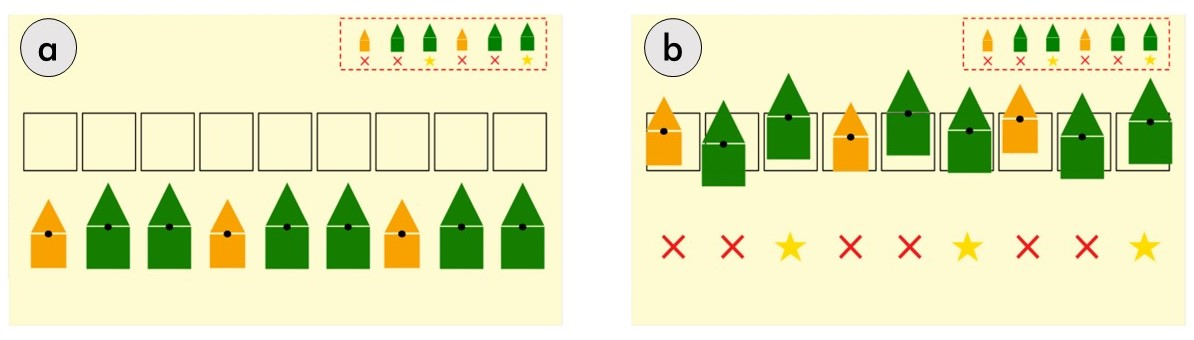
\includegraphics[width=0.9\textwidth]{future/figures/pattern_learn.jpg}
  \caption[The pattern learning task consists of three units of an ABB pattern with house shapes and a small icon to remind children of the underlying pattern.]{a) The pattern learning task consists of three units of an ABB pattern with house shapes and a small icon to remind children of the underlying pattern. b) Children can reveal the contents of the houses to to find the hidden stars underneath. \textit{Exploration} condition children chose the order in which the houses were revealed while \textit{demonstration} condition children watched the experimenter reveal the houses in the order of their age-matched \textit{exploration} counterpart.
}
  \label{fig:pattern-learn}
\end{figure}

\textit{Pattern Learning Task.} The pattern learning task consisted of a row of nine house shapes of two sizes and colors: the orange houses were small shapes, and the green houses were big shapes. The nine houses formed a three-unit ABB pattern (small, large, large) (Figure \ref{fig:pattern-learn}a). The second `B’ shape in each ABB unit contained a star shape hidden underneath with all other house shapes hiding an 'x' underneath (Figure \ref{fig:pattern-learn}b). We informed all participants that their goal was to find the three stars by figuring out the pattern to find them. Participants in the \textit{exploration} chose the order in which to reveal the hidden contents of the nine house shapes. For the \textit{demonstration} condition participants, the experimenter moved all shapes for the participant in the same order as the participant’s paired \textit{exploration} condition counterpart. 

\textit{Pattern Transfer Task.} The pattern transfer task consisted of the same ABB pattern row as the pattern learning task, but with different shapes of different colors (red and purple lightbulbs)(Figure \ref{fig:pattern-transfer}a). As with the learning pattern, stars were hidden under the second B shape in each ABB unit (Figure \ref{fig:pattern-transfer}b). The experimenter explained that the participant could find the stars in the same place using the same pattern as the pattern learning task. A small thumbnail in the corner of the slide served as a reminder of the previous pattern from the learning task. The experimenter gave children five chances to try to find the three hidden stars, giving verbal feedback after each attempt. All children were told to choose five shapes even if they found all three stars prior to the fifth attempt.

\begin{figure}
\centering
  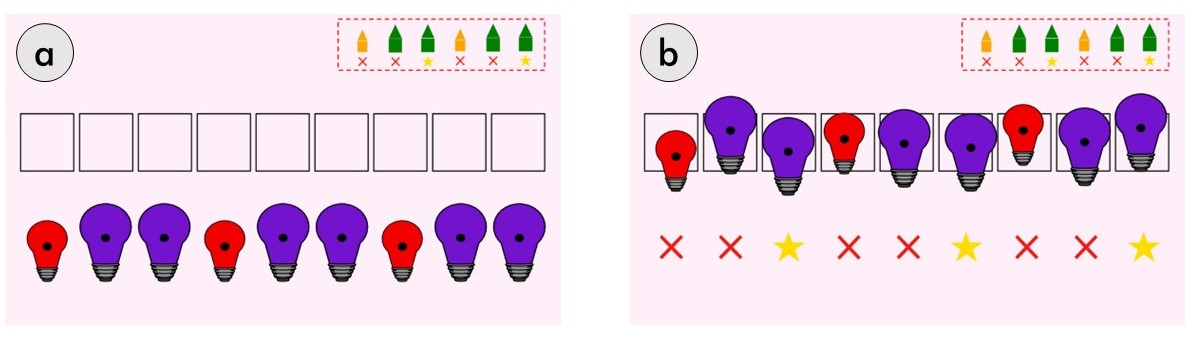
\includegraphics[width=0.9\textwidth]{future/figures/pattern_transfer.jpg}
  \caption[The pattern transfer task consisted of the same three-unit ABB pattern as the pattern learning task.]{a) The pattern transfer task consisted of the same three-unit ABB pattern as the pattern learning task with different shapes. b) Children had five chances to reveal any of the shapes to find the three hidden stars. A small icon in the corner reminded children of the pattern from the pattern learning task.
}
  \label{fig:pattern-transfer}
\end{figure}

\subsection{Preliminary Results}

\begin{figure}
\centering
  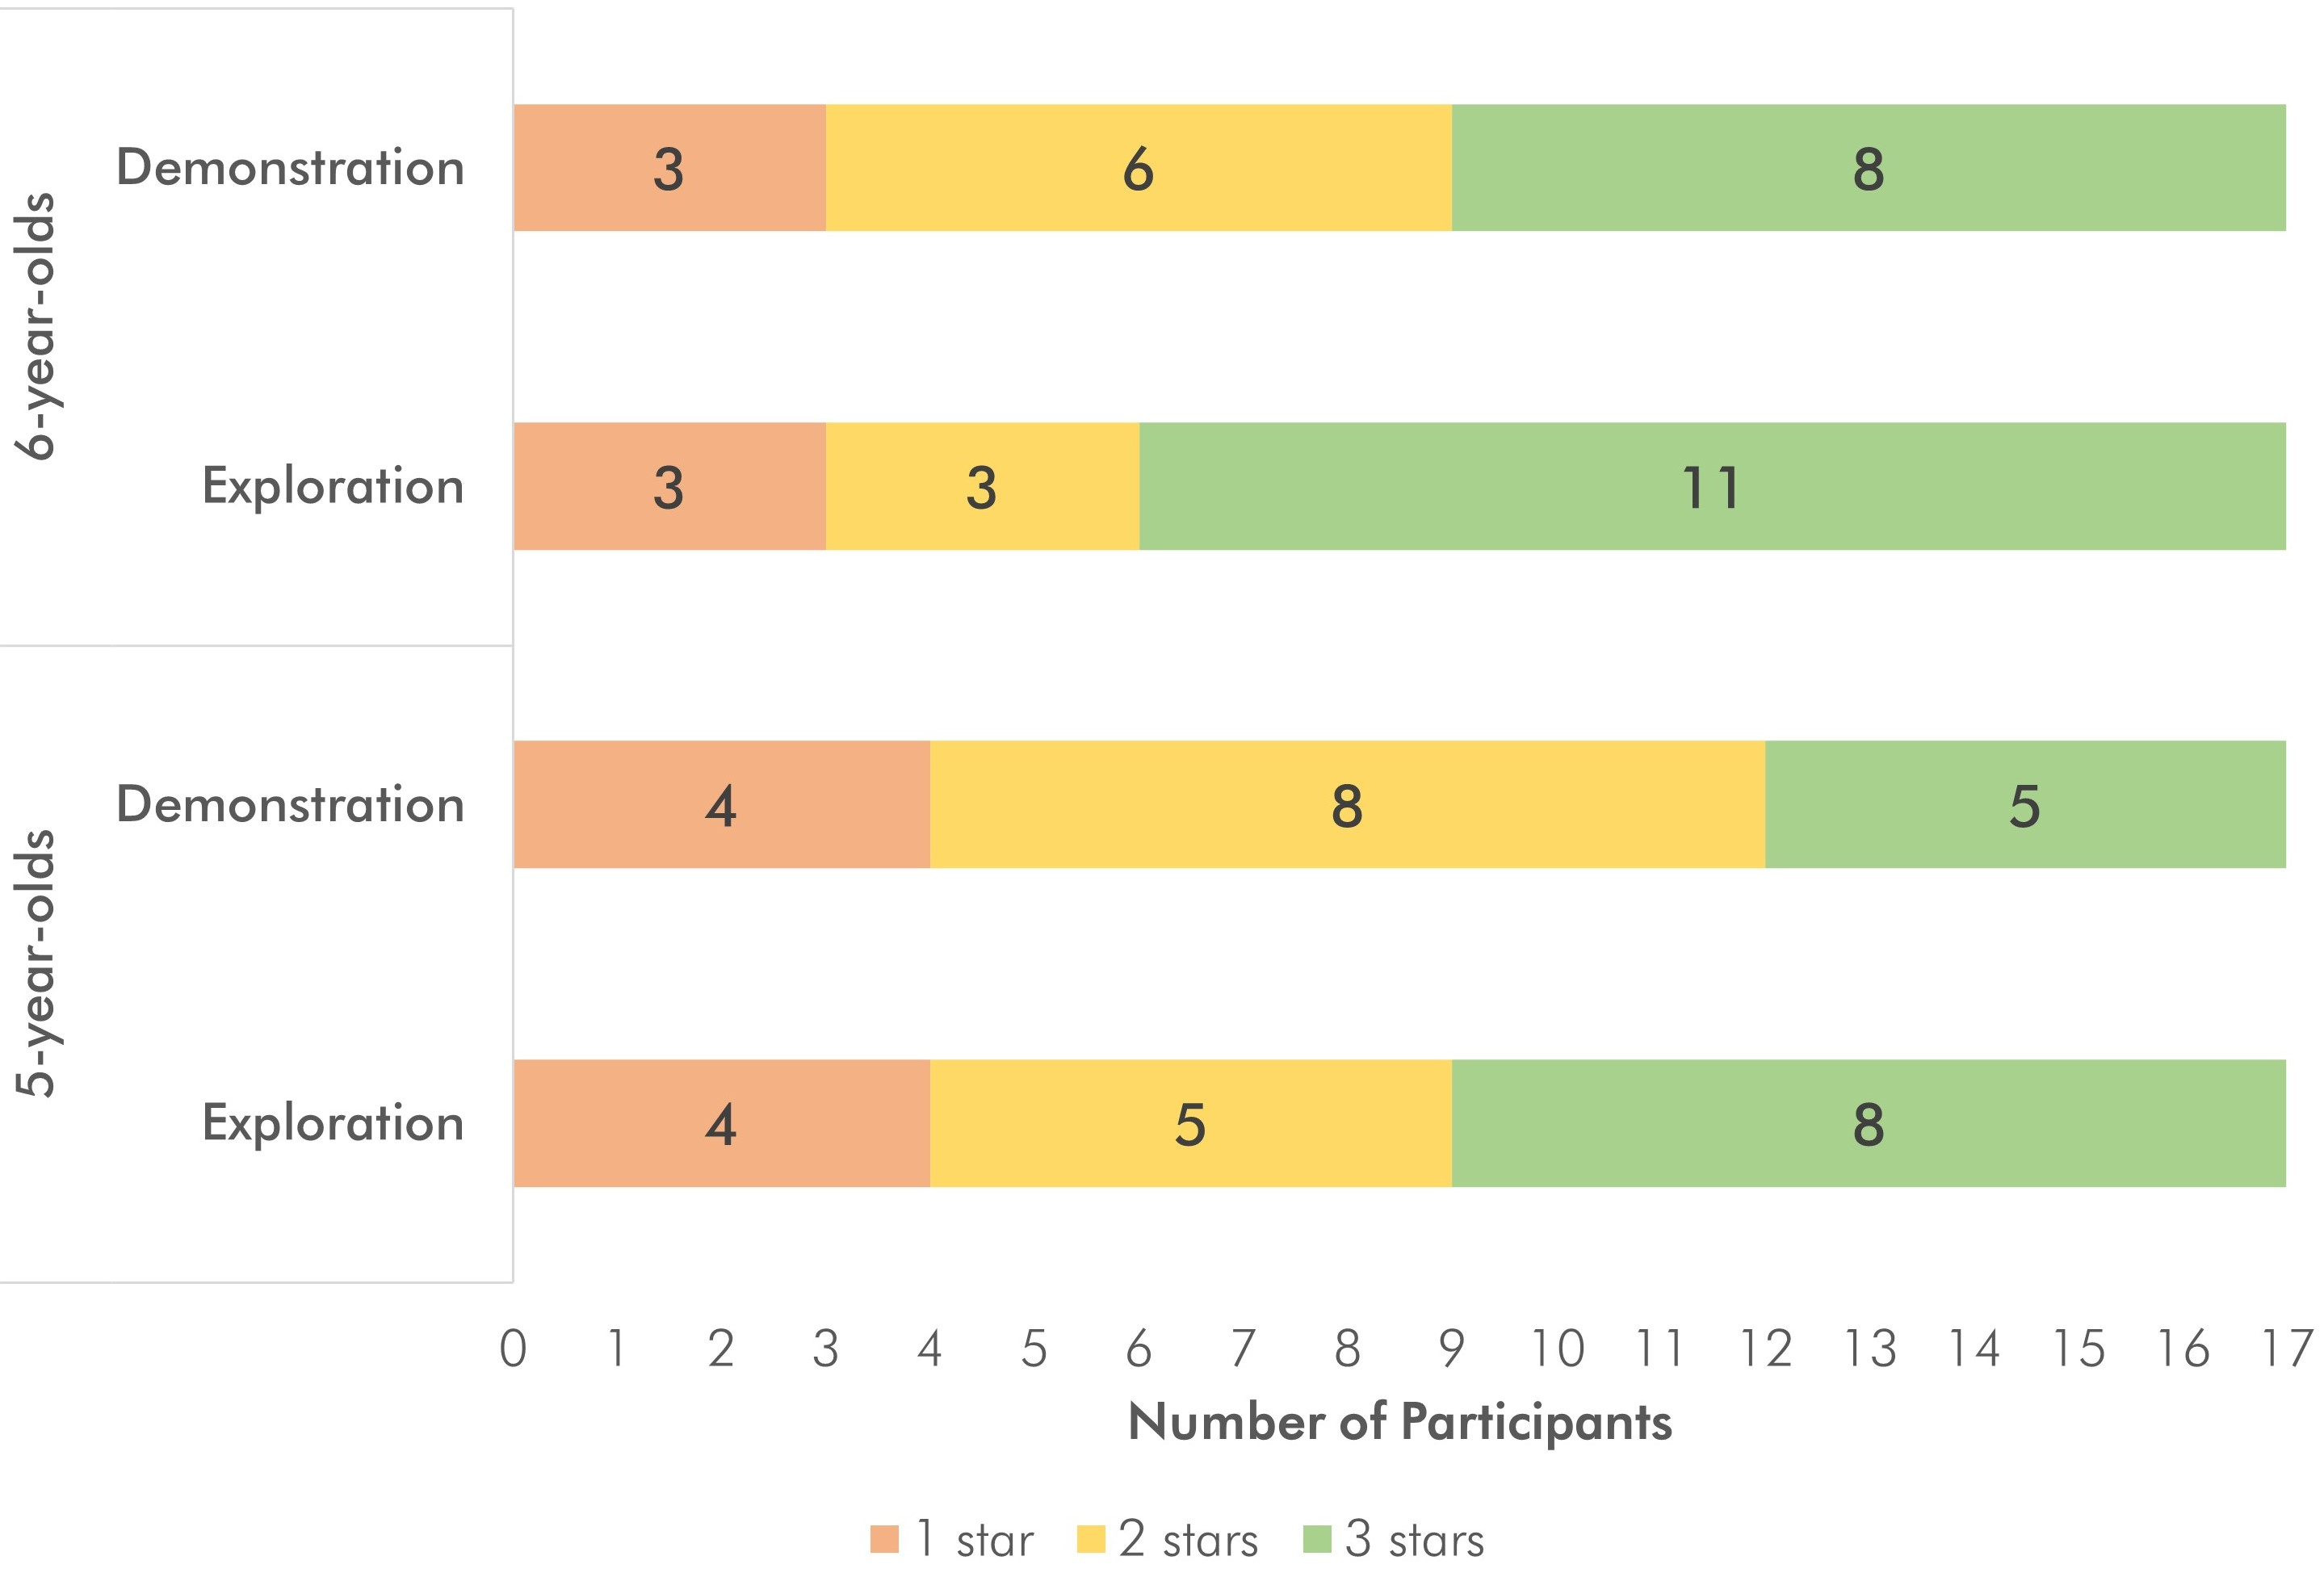
\includegraphics[width=.8\textwidth]{future/figures/pattern_stars.jpg}
  \caption{The number children who found one, two, and three hidden stars in the pattern transfer task ($n=17$ for each age group in both conditions; $n=34$ total in each condition). In both conditions, more six-year-olds successfully found all three stars compared to five-year-olds.
}
  \label{fig:pattern-stars}
\end{figure}

\subsubsection{No significant difference in pattern abstraction}
Pre- and post-test tasks were scored as a binary outcome for whether the pattern was correct or incorrect. We combined the two pre-tests and the two post-test scores into one pre-test and one post-test score with a total out of two for each. Children in both conditions performed nearly at ceiling for both pre- and post-abstraction tasks (\textit{exploration} pre-test $mean=1.79$, $SD=0.54$; post-test $mean=1.82$, $SD=0.52$. \textit{demonstration} pre-test $mean=1.91$, $SD=0.29$; post-test $mean=1.94$, $SD=0.24$). A linear regression with age as a covariate shows that the average difference from pre- to post-test was not significantly different ($F(2,65)=1.76, R^2=0.05, p=.18$).

\subsubsection{Six-year-olds recognize patterns better than five-year-olds}
In general, six-year-olds performed better on the pattern transfer task, with a larger proportion finding all three stars, demonstrating an understanding of the unit of repeat in the ABB pattern. In the \textit{exploration} condition, 8 of the 17 five-year-olds found all three stars compared to 11 of the 17 six-year-olds. In the \textit{demonstration} condition, 5 of the 17 five-year-olds found all three stars compared to 8 of the 17 six-year-olds. All participants found at least one star in the task. Figure \ref{fig:pattern-stars} shows the number of participants who found one, two, and three stars by age and condition. Though there are no significant differences between conditions in the preliminary data ($\chi^2=2.76, df=2, p=.25$), we observed a slight trend towards better performance in the \textit{exploration} condition.

\subsubsection{Exploration affects pattern learning strategies}

\begin{figure}
\centering
  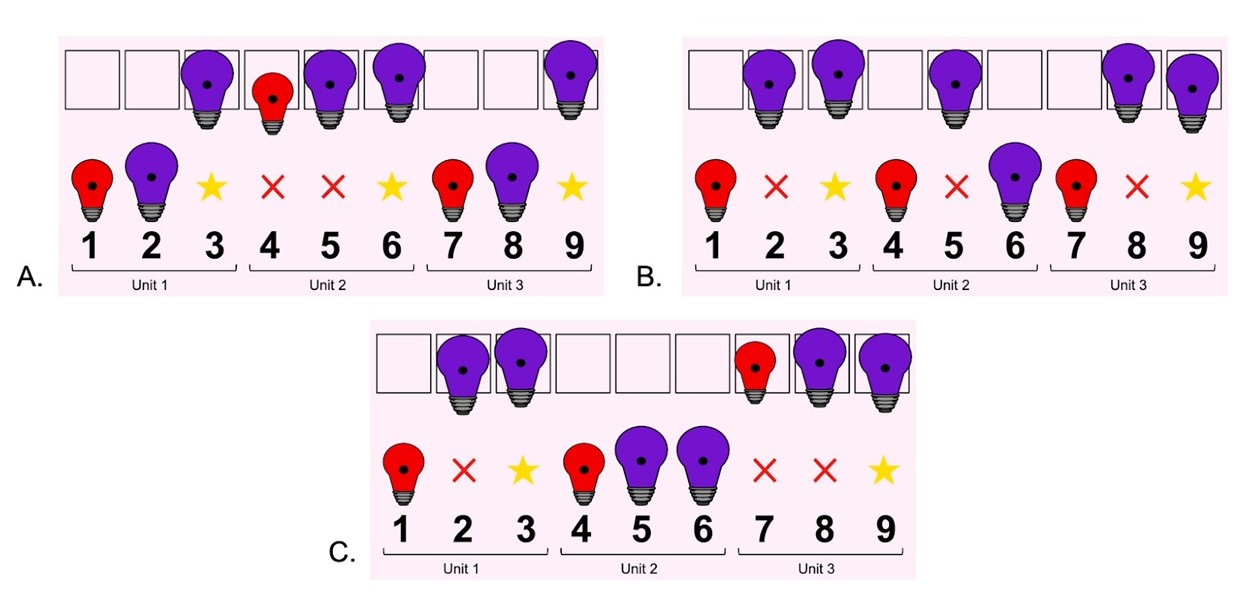
\includegraphics[width=\textwidth]{future/figures/pattern_strat.jpg}
  \caption[Examples of the pattern-relevant strategies.]{Examples of the pattern-relevant strategies observed in the pattern transfer task: A) Unconstrained chunking - searching under at least one shape from all three repeated units, B) Shape matching - searching only under the large shapes, and C) Constrained chunking - searching under shapes from only two of the three repeated units.
}
  \label{fig:pattern-strat}
\end{figure}

Though there were no significant differences in performance on the pattern abstraction task, children interestingly used different strategies. One researcher and a research assistant coded children's patterning strategies blind to condition according to three main categories: pattern-irrelevant, pattern-relevant, and advanced pattern strategies. Disagreements and sub-strategies were discussed and resolved between the two raters. A sequential strategy (choosing shapes from either left to right or right to left in a sequential order) and spatial grouping (searching only in closely proximal shapes) represented the two sub-strategies in the pattern-irrelevant strategies as they do not demonstrate an understanding of the underlying pattern. Unconstrained chunking (searching at least one shape in each of the three repeating units)(Figure \ref{fig:pattern-strat}A), shape matching (searching only in the B shapes in each ABB unit)(Figure \ref{fig:pattern-strat}B), and constrained chunking (searching at least one shape in only two of the three repeating units)(Figure \ref{fig:pattern-strat}C) represented the three pattern-relevant strategies as they demonstrate some understanding of the underlying pattern. Exploit (finding all three stars in a row) represented the most advanced strategy as it demonstrates a clear understanding of not only the underlying pattern, but also the understanding of where each star is within the pattern. Table \ref{table:pattern_strats} shows the various patterning strategies and the frequency of participants who engaged in each strategy. 

\begin{table}[]
\centering
\caption{Children engaged in various strategies to solve the pattern transfer task. In both
the \textit{exploration} and \textit{demonstration} conditions, six-year-olds engaged in more mature, pattern-relevant
strategies than five-year-olds.}
\label{table:pattern_strats}
\begin{tabular}{rrcccc}
\hline
\multicolumn{1}{c}{Strategy Type} & \multicolumn{1}{c}{Sub-Strategies} & \multicolumn{2}{c}{5-year-olds} & \multicolumn{2}{c}{6-year-olds} \\
\multicolumn{1}{l}{} &  & \multicolumn{1}{l}{Explore} & \multicolumn{1}{l}{Demonstrate} & \multicolumn{1}{l}{Explore} & \multicolumn{1}{l}{Demonstrate} \\ \hline
Pattern-Irrelevant & Sequential & 1 & 5 & 2 & 1 \\
 & \begin{tabular}[c]{@{}r@{}}Spatial \\ Grouping\end{tabular} & 3 & 2 & 0 & 1 \\ \hline
Pattern-Relevant & \begin{tabular}[c]{@{}r@{}}Unconstrained\\ Chunking\end{tabular} & 7 & 5 & 7 & 8 \\
 & \begin{tabular}[c]{@{}r@{}}Constrained\\ Chunking\end{tabular} & 1 & 1 & 0 & 1 \\
 & \begin{tabular}[c]{@{}r@{}}Shape\\ Matching\end{tabular} & 2 & 2 & 1 & 2 \\ \hline
Advanced & Exploit & 3 & 2 & 7 & 4 \\ \hline
\end{tabular}
\end{table}

For five-year-olds in both conditions, a majority of children used pattern-relevant strategies in the pattern transfer task (10 out of 17 for the \textit{exploration} condition and 9 out of 17 for the \textit{demonstration} condition). A majority of six-year-old \textit{demonstration} condition participants also used pattern-relevant strategies (11 out of 17). 7 of the 17 six-year-old \textit{exploration} condition participants used the most adavanced exploit strategy, finding all three stars consecutively, compared to 4 of the 17 six-year-old \textit{demonstration} condition participants. These preliminary results suggest that exploration may influence implicit pattern recognition and lead to better transfer and abstraction of patterns in new contexts.

\subsection{Discussion}
We provide preliminary evidence of the efficacy of utilizing exploration as a learning strategy in patterning for young children. This section discusses how exploration can further impact pedagogical methods and learning outcomes for children.

\subsubsection{Exploration Encourages Active Engagement}
Our results demonstrate that children can implicitly learn patterns even without direct instruction or feedback. As opposed to the \textit{demonstration} condition, exploration enabled children to make sense of the pattern on their own. This active engagement may be a reason why we observed a trend of more \textit{exploration} condition children engaging in an advanced, exploit strategy in the pattern transfer task. Because they were able to engage with the pattern previously, they may have been better able to connect the two structurally similar patterns. 

Some children spontaneously explained their pattern reasoning during the pattern transfer task. For example, one five-year-old \textit{exploration} participant said during the pattern transfer task, ``\textit{It looks like a pattern right? Listen, it’s star, x, x, star, x, x, star, x, x.}'' Similarly, a six-year-old in the \textit{demonstration} condition referred to the pattern from right to left and explained, ``\textit{This is the pattern. It’s no star, no star, star, no star, no star, star, no star, no star, star}.'' Other children also pointed out the star and x pattern, but did so with respect to the shapes. For example, a five-year-old in the \textit{exploration} condition stated, ``\textit{After two houses, one house has a star inside of it}.'' A 6-year-old in the \textit{exploration} condition similarly expressed, “\textit{Wait, I realized something. There’s a pattern: two houses that don’t have a star and then one house that does have a star}.” Both children successfully found all the hidden stars using the advanced exploit strategy. Though not explicitly told the pattern to finding the hidden stars, both five- and six-year-old children demonstrated knowledge of the underlying pattern. More specifically, they showed understanding of the repeating pattern unit. Future interventions that utilize active engagement through exploration show promise for developing a general ability to identify repeating units within a pattern even without direct instruction.

Our study examined the immediate learning effects of exploration. Future work could examine the longitudinal effects of using exploration as a learning strategy. For example, inventive activities that ask learners to produce original solutions prior to direct instruction prepare learners for future learning because they can connect their preconceptions to new knowledge gained \cite{Schwartz2004}. Exploratory learning strategies may have a similar impact, priming children to pay attention to the high-level pattern structure rather than the specific components (\textit{i.e.} shapes or stimuli) of the pattern. 

\subsubsection{Exploration Needs to Be Goal-Directed}
Exploration as a problem-solving strategy can be inefficient, particularly when the goal itself may be ambiguous \cite{fraser2019replay,kirschner2006,tuovinen1999comparison}. In our task, children had a clear goal to accomplish: find the hidden stars using a pattern. With this goal, children were directed in their exploratory efforts, which emerged through the strategies we observed. In addition, the task included immediate feedback. Children could see whether the house they selected contained a star underneath right after selection. This feedback may have helped children test and update their hypotheses of the pattern \cite{sumner2019,wilson2021}. While the pattern for finding the hidden stars was concrete, the differing strategies children used suggest that goal-directed exploration and immediate feedback may highlight alternative paths to solving the pattern. 28 of the 34 children in the \textit{exploration} condition and 23 of the 34 children in the \textit{demonstration} condition used some form of pattern-relevant strategy, demonstrating some understanding of the underlying pattern unit. In other forms of creative problem-solving, exploratory strategies should similarly enable people to quickly receive feedback and provide a clear goal to achieve through exploration.

\subsubsection{Summary}
We investigated whether exploration could help children learn and transfer patterns. In a between-subjects experiment, children either explored patterns themselves or watched a demonstration of the pattern. Our results suggest a trend that exploration may encourage more active engagement and highlight underlying structure. Future interventions that utilize exploration as a problem-solving strategy should provide mechanisms for immediate feedback and goal direction.

\subsubsection{Acknowledgements}
We thank our participants and their families for the time and participation in this task. We also thank Amberley Stein for assisting with coding patterning strategies.

This chapter, in part, is currently being prepared for submission for publication of the material by Tricia J. Ngoon, Vivian Leung, and Caren M. Walker. The dissertation author was the primary investigator and author of this material.

\section{Problem-Framing Scaffolds: Hot \& Cool Thinking \\in Creativity}
\label{sec:hats_exp}
Effective creative work requires both ``hot'' (exploratory) and ``cool'' (exploitative) thinking. Unfortunately, many people (especially novices) under-explore, jumping to the ``cool'' part too quickly, because they assume their current thinking ``has to be'' the path.  This paper presents empirical results of how metaphorical problem framing scaffolds can influence creative performance. The task used De Bono's ``Thinking Hats.'' In a between-subjects experiment comparing exploratory to exploitative problem frames, the exploratory problem frame led to more original designs and more diverse ideas during brainstorming. This work provides an empirical baseline of how -- even for short tasks -- assigning people responsibility for broad thinking leads to better creative work.

\subsection{Why are people so often averse to exploration?}
Problem-solving engages a cycle of ``hot'' (exploratory) and ``cool'' (exploitative) thinking, searching broadly before narrowing onto any single idea or solution \cite{kirkpatrick1983optimization,lucas2014children}(Figure \ref{fig:sim-ann}). People often \textit{satisfice}, stopping at the first solution they consider to be good enough \cite{simon1972theories}. Often, this is a savvy way to save time. However, the dark side of satisficing is when people underestimate the space of possibility, as often happens with complex creative problems, quickly settling on a path means forgoing (unconsidered) options that could be much better.  

\subsubsection{Strategies for Increasing Early Exploration Help to an Extent}

To encourage broader exploration early in problem-solving, brainstorming, process models like the Double Diamond, and design thinking approaches encourage wild ideas at the outset. Despite this explicit encouragement, people -- especially novices -- still under-explore. The tendency to cool too soon and fixate can be difficult to overcome. Iteration and examples alone do not necessarily mean greater divergence as people tend to explore within a narrow solution space \cite{Dow2009, jansson1991design, kulkarni2012early}. Without domain knowledge or strategies for exploration, people systematically underestimate how many better ideas are out there. 

% \begin{marginfigure}[5\baselineskip]
%   \begin{minipage}{\marginparwidth}
%     \vspace{-8cm}
%     \centering
%     \includegraphics[width=\marginparwidth]{images/green.png}
%      \includegraphics[width=\marginparwidth]{images/blue.png}
%     \caption{The green thinking hat represents exploration; the blue thinking hat represents exploitation.}

%     ~\label{fig:hats}
%   \end{minipage}
% \end{marginfigure}

\subsubsection{How Do We Overcome Satisficing?}
% \subsection{How Might We ``Set the Temperature'' of Creative Thought?}
We hypothesize that more explicitly attending to exploration and exploitation as phases may improve creativity. Approaches like brainstorming offer psychological safety and improve group's collective knowledge by ``encouraging wild ideas'' and ``deferring judgment.'' One potential advantage of design thinking and related methods is that seeing problems from a user's perspective and drawing inspiration from existing practices and challenges gives people a different vantage point from which to see ideas \cite{debono1985, Dow2009, teevan2017}. To \textit{harness} better ideas, one must first see them. Despite compelling advances from leading practitioners, the empirical basis for stretching people's horizons remains limited. 

This section explores the benefits of asking people to simply ``look further,'' and also provides a more cognitive account of process than is available in the practitioner literature. We present a between-subjects study comparing an explore problem-framing scaffold to an exploit problem-framing scaffold. We found that with an exploratory framing, people provide more original designs and show greater diversity of ideas during brainstorming. This section demonstrates how process scaffolds connect to design outcomes and can ``set the temperature'' in creative thinking. 

\subsection{Experiment 1: Can Problem-Framing Scaffolds Influence Creative Thought?}

\subsubsection{Method}
This between-subjects experiment establishes a baseline of whether it is possible to influence creative outcomes by scaffolding how to frame problems. We adapt our scaffolds from DeBono's \cite{debono1985} Thinking Hats. These ``hats'' provide a metaphor for particular roles and purviews. DeBono's Green Hat represents creativity and serves as our explore scaffold (Figure \ref{fig:hats}a); the Blue Hat represents action and goal-setting and serves as our exploit scaffold (Figure \ref{fig:hats}b). We hypothesized that the explore scaffold would lead to more original ideas and broader search during the brainstorming period while the exploit scaffold would lead to more practical, but less original ideas and narrower search during the brainstorming period.

\begin{figure}
\centering
  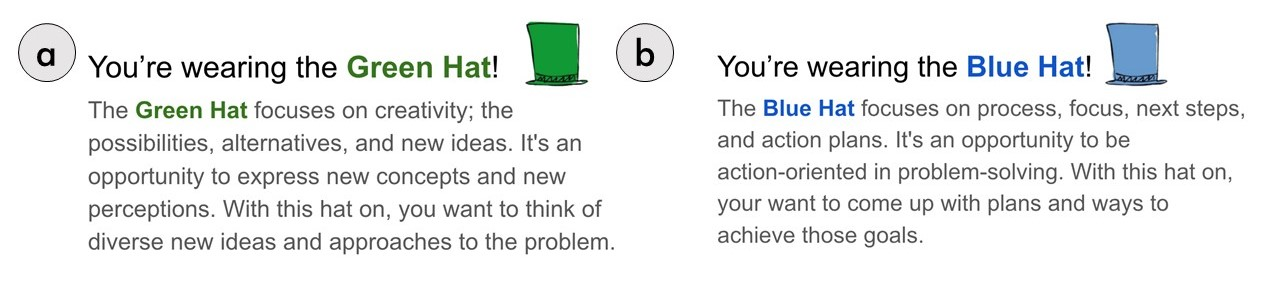
\includegraphics[width=\textwidth]{future/figures/thinking_hats.jpg}
  \caption{a) The green thinking hat represents exploration, and b) the blue thinking hat represents exploitation. Participants in Experiment 1 used these scaffolds during brainstorming.
}
  \label{fig:hats}
\end{figure}

34 participants (27 female) were recruited from the Psychology \& Cognitive Science subject pool (SONA) at a California research university. This task asked participants to redesign an aspect of the student eating experience to be better or more enjoyable. All participants received this scenario; half were randomly assigned to an \textit{Explore} frame, half to an \textit{Exploit} frame during the brainstorming period. The experiment gave five minutes for initial brainstorming and ten minutes to write a description of their preferred idea, why it is unique, and why it would improve the student eating experience. Lastly, a written survey asked participants questions about their experience with the Thinking Hat scaffolds.

\begin{figure}
\centering
  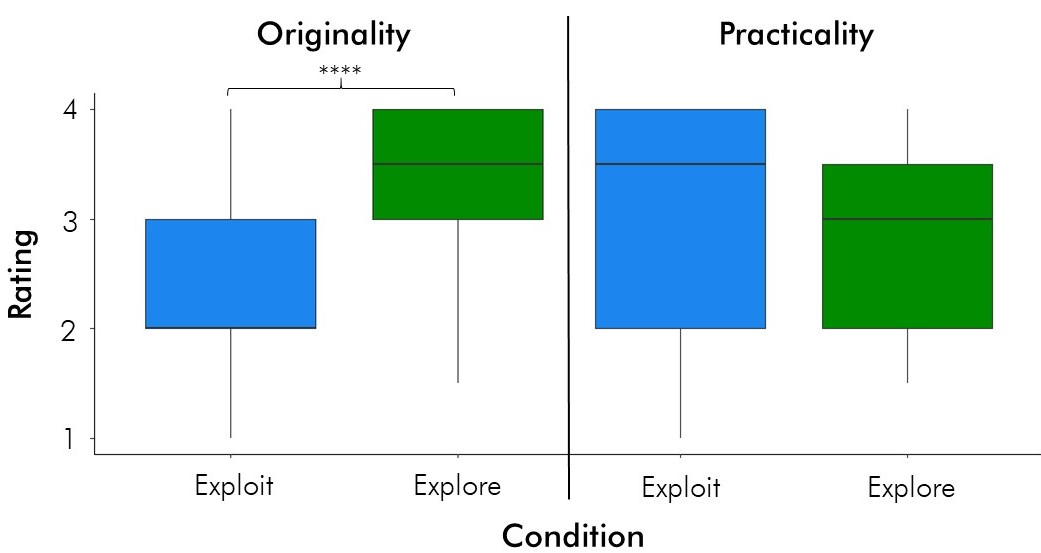
\includegraphics[width=\textwidth]{future/figures/baseline.jpg}
  \caption{Participants with the \textit{Explore} framing ($n=17$) received significantly higher originality ratings for their designs than the \textit{Exploit} framing ($n=17$). There were no significant differences between practicality ratings. ****$F(1,48)=15.2, R^2=0.22, p<.001$
}
  \label{fig:baseline}
\end{figure}

\subsubsection{Exploratory Framing Leads to More Original Designs \& More Diverse Ideas}
Two expert raters blind to condition with knowledge of campus issues and dining spaces rated each design on a 4-point Likert Scale for \textit{originality, practicality}, and \textit{justification} (how well motivated the design is). The inter-rater reliability between raters was substantial (${\kappa}=0.61$) Ratings were averaged between both raters for originality and practicality. \textit{Explore} condition designs received significantly higher average ratings for originality ($m=3.3, SD=0.75$) than \textit{Exploit} condition designs ($m=2.4, SD=0.88$)($F(1,48)=15.2, R^2=0.22, p<.001$). Contrary to our hypothesis that the exploit scaffold would lead to higher practicality ratings, there were no significant differences between conditions for practicality ratings (\textit{Explore} $m=2.82, SD=0.86$; \textit{Exploit} $m=3.02, SD=0.93$)($F(1,48)=0.62, R^2=-0.01, p=.43$) between both conditions (Figure \ref{fig:baseline}). 

The expert raters also assessed the diversity of each participant's ideas on a 4-point Likert scale. Highly similar ideas (\textit{i.e.} ``make buffet-style payment system,'' ``give students a certain number of swipes on payment cards'') earned a 1 while highly diverse ideas (\textit{i.e.} ``chefs for students included in tuition,'' ``grocery buddies/cooking mentors'') earned a 4 on this scale. \textit{Explore} participants ($m=3.02, SD=1.05$) brainstormed significantly more diverse ideas than \textit{Exploit} participants ($m=2.04, SD=0.99$)($F(1,48)=11.6, R^2=0.18, p<.005$) (Figure \ref{fig:diversity}). 

\begin{figure}[b!]
\centering
  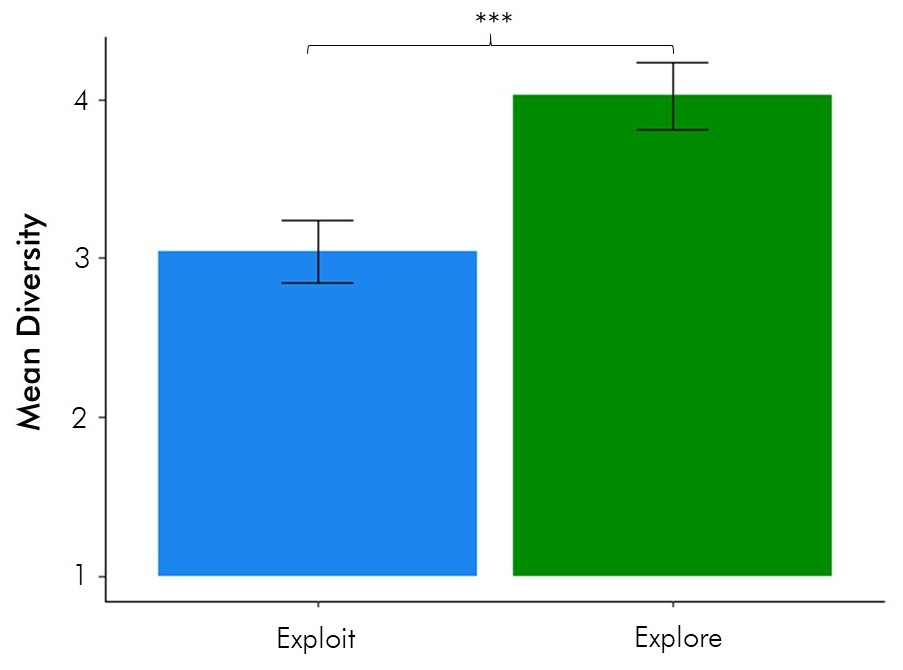
\includegraphics[width=.7\textwidth]{future/figures/diff.jpg}
  \caption{Participants with the \textit{Explore} ($n=17$) framing demonstrated greater diversity in their brainstormed ideas than those with the \textit{Exploit} ($n=17$) framing. ***$F(1,48)=11.6, R^2=0.18, p<.005$
}
  \label{fig:diversity}
\end{figure}

\subsubsection{Exploratory Framing Enhances Perceptions of Creativity}
The explore scaffold particularly helped participants push their boundaries of thought. One \textit{Explore} participant stated that the without the Thinking Hat, \textit{``I may have gotten to the same ideas..., but I probably would have refuted them on the spot with a reality check, or doubt.''} Another stated that the scaffold \textit{``made me question myself and think harder about the possibilities}.'' Two participants mentioned that the Thinking Hat as a metaphor was a particularly helpful metaphor. One participant said, \textit{``The green hat had a placebo effect on me..., which influenced me to think outside the box and use my creativity regardless of feasibility.''} Another stated that, \textit{``I could actually visualize wearing the hat [while] brainstorming new ideas.''} One participant even said the thinking hat itself served as inspiration for his design. 

\subsubsection{Exploit Framing Encourages Real-World Action}
Eight \textit{Exploit} participants mentioned that the problem frame scaffold helped with organizing and structuring their thoughts towards goal-oriented solutions. One \textit{Exploit} participant said the scaffold \textit{''made me think about how [my ideas] could be practically accomplished, since it seemed to emphasize real-world action.''} The exploit scaffold also seemed to be similar to participants' existing problem-solving strategies. Four participants believed their process of problem-solving without the thinking hat would have been the same. As one participant said, \textit{``I think the blue thinking hat already describes my thinking process..., so I didn't have to constantly remind myself to think a certain way or use different methods to think.''} None of the \textit{Exploit} participants mentioned that the scaffold was challenging; they all felt that it added or supplemented their ideation. However, one \textit{Exploit} participant felt the framing limited his thinking, stating that it ``\textit{restricted him to analytical thinking versus being creative.''}

\subsection{Experiment 2: Does the Order of Explore \& Exploit Affect Creative Outcomes?}
\subsubsection{Method}
A second experiment examined whether the order of the explore and exploit problem framing would impact creative outcomes. In this between-subjects study, 48 participants (30 female) from a California research university were recruited from an undergraduate design course. Similar to the first experiment, participants redesigned an aspect of the student eating experience. The task consisted of two initial brainstorming phases where participants used either explore or exploit scaffolds, the order of which was randomly counter-balanced between participants (23 participants in the \textit{Explore-Exploit} condition, 25 participants in the \textit{Exploit-Explore} condition). After each brainstorming phase, participants wrote a design idea, with the second design idea being the final design. Participants answered general questions about their experience in a post-survey after the experiment. 

%Don't center
% Participants in the Explore-Exploit condition (n=xx) were given the Explore prompt during brainstorming first while participants in the Exploit-Explore condition (n=xx) were given the Exploit prompt during brainstorming first. 

\subsubsection{Explore Framing Improved Originality of First Design}
Two experts in the food service industry blind to condition rated the final designs on two dimensions of \textit{Originality} and \textit{Practicality}, each on a 4-point Likert scale. Scores for each time point were averaged between both raters. The inter-rater reliability for raters was substantial (${\kappa}=0.69$). \textit{Explore-Exploit} participants received higher average originality ratings for their first design than \textit{Exploit-Explore} participants ($F(1,46)=8.1, R^2=0.13, p<.01$). There were no significant differences in originality ratings between conditions for the second design ($F(1,46)=1.08, R^2=.002, p=.30$). There were also no significant differences in practicality ratings between conditions for both the first ($F(1,46)=0.32, R^2=-0.01, p=.58$) and second designs ($F(1,46)=0.15, R^2=0.02, p=.70$)(Figure \ref{fig:order}). As this work is preliminary, our results suggest a trend for further investigation.

\subsubsection{Exploratory Scaffold Encouraged Wild Ideas}
Despite our observed null quantitative results for most measures, the explore scaffold seemed successful in challenging participants to think more creatively based on qualitative reports. One participant in the \textit{Explore-Exploit} condition noted, \textit{``it pushed me to think of designs from different perspectives and points of view.''} Similarly, one participant in the \textit{Exploit-Explore} condition thought the explore scaffold \textit{``opened the gates to better, more refined ideas.''} 

\begin{figure}
\centering
  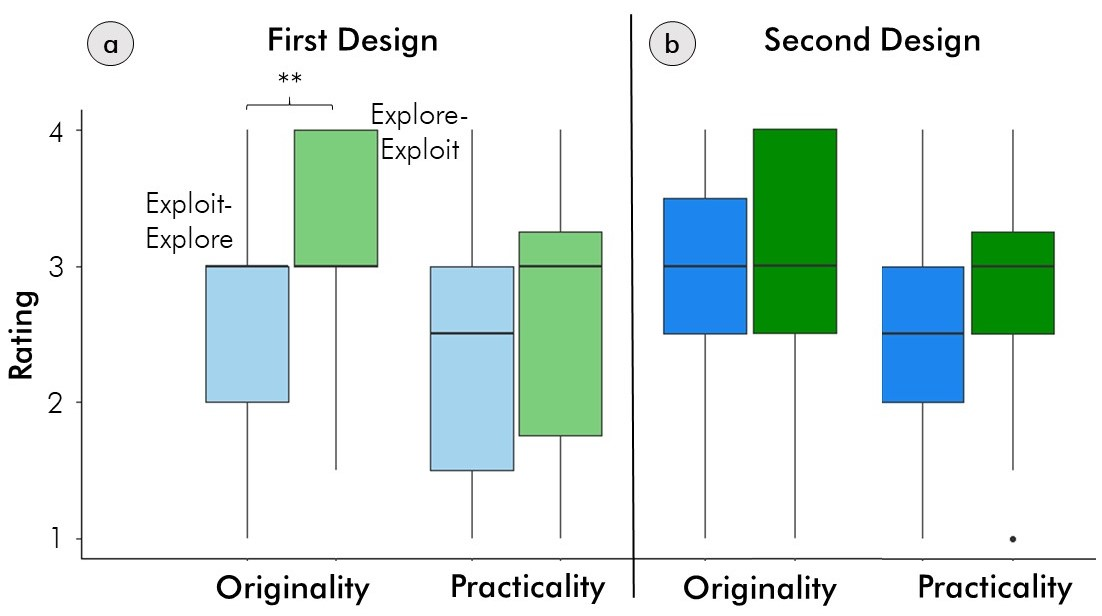
\includegraphics[width=.9\textwidth]{future/figures/order.jpg}
  \caption[a) Participants with the \textit{Explore-Exploit} order ($n=23$) received higher originality ratings for their first designs than \textit{Exploit-Explore} ($n=25$) participants, but not differences in practicality ratings.]{a) Participants with the \textit{Explore-Exploit} order ($n=23$) received higher originality ratings for their first designs than \textit{Exploit-Explore} ($n=25$) participants, but not differences in practicality ratings. b) We observed no significant differences in design outcomes for either measure in the second designs. A larger sample size or a change to the scaffolds themselves might result in more pronounced effects. **$F(1,46)=8.1, R^2=0.13, p<.01$
}
  \label{fig:order}
\end{figure}

Some participants in both conditions thought the explore scaffold was challenging, but ultimately useful for creativity. For example, one \textit{Explore-Exploit} participant said, \textit{``it was shocking, but after the initial shock it helped spur a lot more creative ideas.''} A participant in the \textit{Exploit-Explore} condition added, \textit{``it forced me to step outside of my comfort zone and see things from a different perspective even if I didn't think that was possible.''} This notion of feeling challenged may enhance creative thought regardless of order. 
\subsection{General Discussion \& Next Steps}
We provide preliminary empirical evidence of how problem framing can nudge people towards different cognitive processes and creative outcomes. This section addresses the implications and ongoing challenges of using this strategy.

\subsubsection{Exploring Broadly is Difficult Without Prerequisite Domain Knowledge}

The inclination to satisfice and find the ``good enough'' solution is particularly strong because of the time saved and effort required \cite{simon1972theories}. In both our experiments, the metaphor of an exploratory Thinking Hat seemed to enhance people's perceptions of their own creativity, which is a promising direction towards increasing productive exploration. Still, many final designs in Experiment 1 were similar to each other across conditions (for example, six designs mentioned sending out surveys for greater variety in dining halls on campus. Unfamiliarity with the domain space and the potential possibilities may have limited novices' ability to come up with fully original ideas. 

Importantly, the explore scaffolds led to increased intra-exploration, where people's ideas during brainstorming were more diverse even if their final design outcome was similar to others. In Experiment 1, \textit{Exploit} participants often came up with highly similar ideas or multiple examples of a single idea. In both experiments, participants frequently reported that the exploit scaffold was useful in structuring their thoughts, but it did not particularly challenge them to think differently. In contrast, many participants found the exploratory framing either challenging or effective in spurring new ideas. It may be that the perception or safety of feeling challenged enhances originality. Additionally, wearing even a metaphorical hat may enable people to play out a ``role'' of exploration or exploitation, similar to prior work on human-centered mindsets \cite{chou2017finding,teevan2017}. Our findings demonstrate that drawing attention to phase (explore or exploit) can influence creative mindset and potentially help in overcoming this tendency to satisfice and exploit early. An interesting area of future study might be examining how to further leverage this intra-exploration, perhaps by explicitly prompting for different perspectives or adding additional problem constraints.

\subsubsection{Early Exploration Can Lead to Better Exploitation}
Despite our hypothesis that a goal-oriented framing would lead to more practical ideas than the exploratory framing, we found no significant differences between the two conditions in both experiments. One potential concern of over-exploration is that wild ideas are produced without any being of practical use. Instead, broad exploration may help people realize the boundaries of a solution space without sacrificing practicality. We found this in Experiment 2 as well. Regardless of order, attending to exploration as a phase seemed fruitful in spurring more creative thought and ideas. 

Exploration may also lead to more concrete and specific ideas. Four designs in the \textit{Exploit} condition of Experiment 1 were overly broad. For example, one design suggested lowering the cost of food as a way to improve the student eating experience. While the design was well justified, it lacked specific details of how it could be put in place. An early exploration phase may indeed be necessary to refine concrete ideas later. This phase might attune people towards originality while maintaining their ability to later further develop and evaluate ideas. Future work should examine how to better scaffold the evaluation process to harness both unique and actionable ideas.

In Experiment 2, we observed that the \textit{Explore-Exploit} condition produced more original first designs with \textit{Exploit-Explore} participants improving slightly in Originality ratings for their second design. This may suggest that prompting for exploration is beneficial regardless of where the person is in their creative process. Just as semantically diverse examples provide the most creative inspiration when a person reaches an impasse \cite{chan2017semantically}, prompts for exploration might be most useful when a person feels stuck or ``out of ideas.'' Interestingly, a simple nudge, while not significant on its own, can at least catalyze getting unstuck.

\subsubsection{What Scaffolds Improve Exploration?}
Creative thinking combines domain knowledge with procedural strategies for greater exploration. Our experiments examine the latter, and our results suggest that how problems are framed affect people's thinking in different ways. Even simple metaphorical scaffolds like the Thinking Hats may be useful strategies in preparing novices to be creative by assigning a ``role'' to be creative. However, novices lack domain knowledge about a problem space and may need further help in understanding what creative means in a particular domain. To supplement this lack of knowledge, examples can provide anchors that usefully constrain a problem space \cite{Dow2009, kulkarni2012early}. Pairing problem framing as an exploratory strategy with the use of examples may aid in eliciting more creative design outcomes. In addition, combining problem framing with more structured exploratory strategies, such as those provided at the Stanford dschool (www.dschool.stanford.edu), can be an effective pedagogical approach for creative learning. 

\subsubsection{Summary}
%summarize experiments and what to do next
We present empirical results of how the framing of problems can ``set the temperature'' of creative thinking. We found that an exploratory framing leads to more diverse ideas and more original design outcomes. The explore scaffold challenged participants to think more freely about a problem; the exploit scaffold helped participants structure and organize their thoughts. Future work should examine how such problem framing can be used with other strategies and scaffolds to catalyze creative learning.

\subsubsection{Acknowledgements}
We thank research assistants Michelle Lee and Nicolas La Polla, study participants, and expert raters. This work was funded in part by NSF award \#1735234.

This chapter, in part, is currently being prepared for submission for publication of the material by Tricia J. Ngoon, Vivian Leung, and Caren M. Walker. The dissertation author was the primary investigator and author of this material.

This chapter, in part, includes portions of material as it appears in \textit{The Dark Side of Satisficing: Setting the Temperature of Creative Thinking} by Tricia J. Ngoon, Caren M. Walker, and Scott Klemmer in the Proceedings of the 2019 ACM Conference on Creativity and Cognition (C\&C '19). The dissertation author was the primary investigator and author of this material.


\chapter{Conclusions \& Future Work: Opportunities for Fostering Creative Learning}
\begin{quote}
    My hope is that this dissertation has demonstrated that attunement benefits creative exploration because knowing how to ``see'' is central to expertise. While simply telling people may not be sufficient (Section \ref{sec:hats_exp}), I believe that richer attunement scaffolds can be highly effective. For example, this dissertation presented a simplification attunement scaffold to help people focus on high-level visual composition (Chapter \ref{chapter:abstraction}), a scaffold for presenting conceptually-relevant examples (Chapter \ref{chapter:shown}), and a scaffold for reusing high-quality examples in improving feedback (Chapter \ref{chapter:critiquekit}). This chapter describes opportunities for future work with these scaffolding strategies.
\end{quote}

\section{Embracing Ambiguity}
I believe that a major roadblock to exploration and creative work is an emphasis on perfection or quantifiable metrics rather than iteration and progression. Creative work by nature is ambiguous, which makes fixating on the salient and the concrete all the more appealing, an ``analysis paralysis'' or choice paradox where so many options are possible that satisficing on one seems like the best solution to avoid being wrong \cite{grant2021think,schwartz2004paradox,simon1972theories}. Part of developing expertise is learning what details to pay attention to and when and not getting lost among the `trees.' For instance, focusing on the perfection of a character's outfit while sketching early on can distract (literally) from the bigger picture. Representations work best when the amount and type of expression they facilitate align well with the goal. One benefit of expertise is being able to break down the larger problems into simpler chunks where novices have greater difficulty in seeing how to do so. Abstraction blocks make concrete the intangible, abstract things that are easy to overlook. We found that groups using abstraction blocks in drawing focused more on composition concepts rather than details like what color a coat should be (Section \ref{sec:abs_study}). The key insight of abstraction blocks is that they make the ambiguous visible and tangible, emphasizing exploration rather than settling on the first known idea. Our study looked at abstraction blocks as an aid for chunking in drawing. Groups that used abstraction blocks formed composition plans with post-it notes as blocks (Figure \ref{fig:abs_drawings}). Abstraction blocks enabled top-down thinking, forming the plan before executing on the details. This draws similarities to backwards design in learning where the overall goal determines the plans and means to achieve that goal \cite{wiggins2005understanding}. 

Setting high-level goals in creative work is difficult because the details distract us in two ways: 1) we do the small stuff to procrastinate from the tougher stuff, and 2) we get so focused on making the small stuff `right' that we can't get past it. I believe the abstraction blocks approach can work domain-generally to help people set high-level goals by removing the details that distract and pigeonhole us.
For example, in writing, focusing too heavily on grammar or wording early on can distract from the high-level narrative and flow of the writing \cite{sommers1980revision}. Abstraction blocks for written work might first start out with blocks for general plot points (\textit{i.e.} conflict and resolution or character development) before the writer begins composing sentences for each block. At an even higher level, what might abstraction blocks look like for making life decisions, like financial planning or figuring out career plans? Can these high-level goals be `chunked' in a way that decomposes the details?

\begin{figure}
\centering
  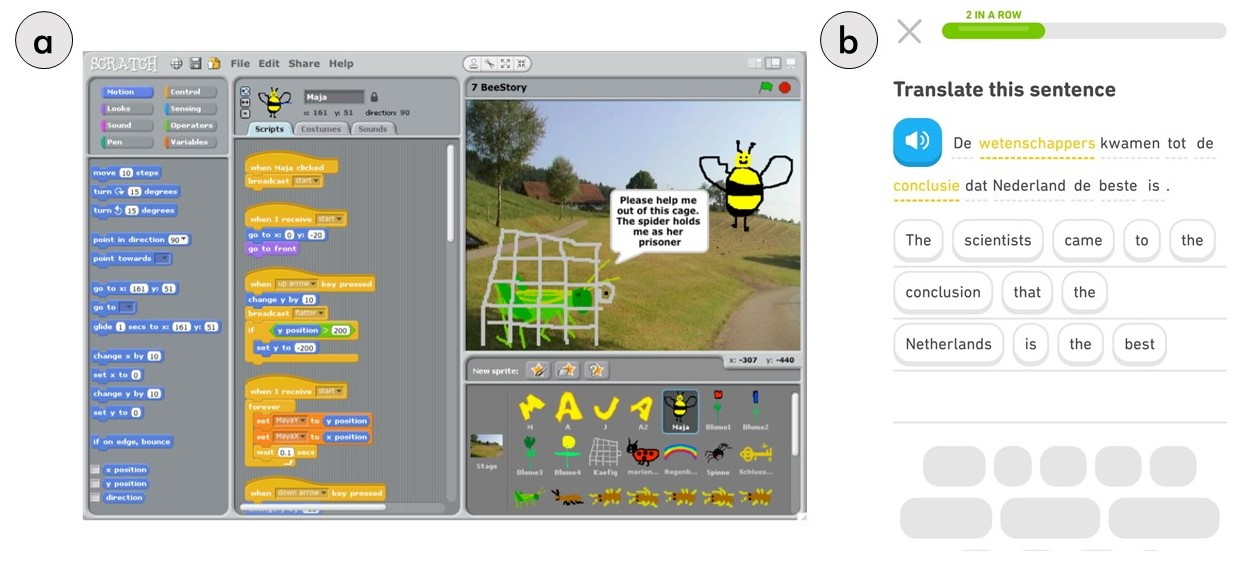
\includegraphics[width=\textwidth]{i_figures/blocks.jpg}
  \caption[Similar to the concept of abstraction blocks, Scratch \cite{Resnick2009} uses block-based programming --short phrases visually rendered into discrete, parameterized blocks-- to help novices easily create games and programs]{Similar to the concept of abstraction blocks, a) Scratch \cite{Resnick2009} uses block-based programming --short phrases visually rendered into discrete, parameterized blocks-- to help novices easily create games and programs by understanding the higher-level concept without worrying about syntax or technical coding details. b) Duolingo \cite{von2013duolingo}(www.duolingo.com) uses blocks to help learners build and translate sentences without the need for minor spelling or grammar concerns.
}
  \label{fig:scratch}
\end{figure}
%make both scratch and duolingo and clearer what the blocks are. In scratch, short phrases visually rendered as discrete, parameterized blocks...in duolingo, blocks to form sentences.

We can look to systems that already use a form of abstraction blocks. Scratch \cite{Resnick2009} and Duolingo \cite{von2013duolingo} incorporate ``blocks'' as physical and moveable instantiations of coding or language learning to make learning more tangible (Figure \ref{fig:scratch}). In our study, abstraction blocks made drawing almost like a puzzle, allowing groups to put the pieces together to create their picture. Finding ways to chunk problems into blocks and scaffolding the process of ``assembling'' them is a promising direction for creativity support tools. For example, tools could provide ``levels,'' where users can toggle between more abstract, malleable chunks and more concrete detailed levels so they can easily shift between exploring the ambiguous and making concrete decisions on the details. Future work should examine how abstraction blocks might be applied as an oblique strategy for scaffolding attention to high-level plans and goals. 

\section{Meeting People Where They Are}
The big vision in education more generally is taking less of a `one-size-fits-all' approach and more of a personalized style to teaching and learning. Someone entering my Cognitive Science graduate program with a mathematics background is going to have a different knowledge base, skillset, and goal than someone with a psychology background, for instance, and the form of training and learning that works best for these two students will look different. The studio-apprentice model and one-on-one tutoring best exemplify this approach where help is adapted to individual learners \cite{bloom1984,Chi2001,schon1984reflective}. In Sch{\"o}n's architecture scenario, the expert explains in detail the choices he makes to the student and engages in a Socratic dialogue \cite{schon1984reflective}. Tailoring learning to one's individual knowledge and goals is tractable for the first time with computers. To emulate this dialogue, Sh{\"o}wn's adaptive conceptual guidance presents general examples to users depending on their actions (Chapter \ref{chapter:shown}). Sh{\"o}wn used predetermined heuristics to decide what conceptual examples to show and when. What if tools could adapt the heuristics to users? 

%prereqs as an example of failure of one-size-fits-all. Someone w/ math background going into phd program vs. psych background and having different goals. Tailoring learning to one's knowledge and goals is for the first time tractable with computers.
%we all come with different knowledge and perceptions, but people don't necessarily learn differently. Make clear 

Every user has individual goals; some want to learn the concepts and gain deliberate practice in a skill while others might want to quickly execute a task without worrying about learning the concepts. Future creativity support tools should provide the most appropriate help for these goals. From our observations with Sh{\"o}wn, we saw that proactive guidance gave novices an awareness of options to consider; user-led, reactive guidance was more useful for small, concrete tasks (Section \ref{sec:shown_exp}). User-led searches are great when you know what to search for, but it's the unknown unknowns that make productive search both unlikely and extremely challenging if you don't know with what you need help. This is where a good tutor, whether a professional or peer, can proactively direct attention to issues you may not have considered and provide new insights. To close the loop, tutors can offer a record of the skills you have mastered and give targeted help for your specific areas of improvement. Similarly, a well-designed adaptive computational tool could proactively suggest help as you need it and create a record of skills you've mastered. Just as a human tutor might give more or less help depending on a learner's progress, tools could also include different modes of help. For instance, a ``maximum help'' mode could provide the most guidance, both for conceptual understanding and technical skill help, while a ``minimum help'' or ``silent'' mode might provide only technical skill help or no help at all. These tools would give freedom to the user to decide which type of guidance they need depending on their own individual goals and tasks. 

%big DEI benefit of computational tutors, with luck, computational coaches can help minimize/counter shortcomings of differing backgrounds.
%A good TA or tutor can recognize which prereq is missing that can lead to another stumbling block. They realize the cause of the error.

\section{Creating Opportunities for Risk-Taking}
Even today, many people hold a folk belief that mathematical abilities are innate rather than learned or grown \cite{rattan2012s}. Similarly, creativity seems to be another attribute that people think of as an innate talent or something accrued through deep experience in a given field rather than in a structured, deliberate manner. This dissertation argues that structured attunement can at the very least catalyze creative exploration and learning. Exploration inevitably includes giving up on some ideas. Most early ideas do not succeed, and the feeling of ``wasting time'' can limit further exploratory efforts. However, wild or even bad ideas can lead to serendipitous discoveries \cite{osborn1953applied}. Creating low-stress and low-stakes environments can encourage exploration and risk-taking. Often, professional and educational settings engender an anxiety that makes people terrified to fail and therefore, terrified to take risks. Risk-taking requires that you can survive the failure. 

Part of taking risks is understanding what aspects are worth the risk and what aspects need iteration. Feedback is a critical piece of this puzzle, learning what works and getting a direction for where to go \cite{Hattie2007,sadler1989formative}. Our work with CritiqueKit showed that reusing exemplar feedback according to the structural critiera of being specific, actionable, and justified can improve feedback quality (Chapter \ref{chapter:critiquekit}). The next step is understanding how feedback is interpreted and applied. In human tutoring and studio models, experts use a variety of representations to explain concepts to a novice, such as sketches or deictic gestures like pointing \cite{goldin1999,schon1984reflective,Tversky2011}. To emulate how an expert might provide feedback to a novice, particularly for visual or multimedia mediums, future feedback tools could allow reviewers to directly demonstrate their suggested improvements through multimodal and deictic interactions. Similar to how ReMap \cite{fraser2020remap} uses deictic gestures and speech queries to find relevant moments in videos to present to users, feedback tools could also use these interactions as context to search for appropriate feedback suggestions from a corpus of critique examples. I hope the direction of critique tools help people both give feedback and better apply it to their work to give people the safety and freedom to take risks in their creative thinking.

% One strategy is to visually show common areas of critique to highlight priorities and show contradicting feedback from reviewers  \cite{yen2020}.

% Capturing good expert and peer feedback and reusing exemplar feedback can foster this community of critique where progression and improvement are emphasized rather than simply achieving a final outcome. 
% Systems like CritiqueKit that reuse previous feedback and scaffold effective and efficient feedback-giving can promote formative improvement rather than summative evaluation \cite{Head2017,Krause2017}. We found that adaptive and interactive feedback reuse drew attention to the structural characteristics of effective critique rather than just the content (Section \ref{sec:critiquekit_exp}).
 
\section{A Future for Computational Coaching}
A few years ago I began working with a boxing coach to improve my proficiency and technique with the goal of sparring more advanced students. My coach saw that despite my smaller size, I have quick footwork, sharp punches, and good handspeed. He tailored his coaching to improve my weaknesses in a way that capitalized on my strengths and showed me alternative ways to handle potential scenarios during a sparring session. Good coaches do exactly this: tailor their efforts to the individual learner and helping them hone their own style. I believe the future of creativity support tools is to emulate coaching, giving people the strategies and tools to accomplish their goals and improve. The future directions I've laid out in this chapter present opportunities to bring us closer to my vision. While this dissertation and other work within creativity support focus on digital learning and creation, an exciting area for computational tools and coaching is in physical domains like woodworking or dance. This dissertation presented three strategies that form the basis for what future computational coaching tools in any domain might become. These tools should provide attentional scaffolding to high-level concepts, adaptive support and relevant examples, and actionable feedback for improvement. We can learn skills and concepts from resources like video tutorials or books, but I believe that learning how to handle open-ended problems and ambiguous scenarios can come from adaptive and interactive guidance from contextualized, personal coaching.

\begin{figure}
\centering
  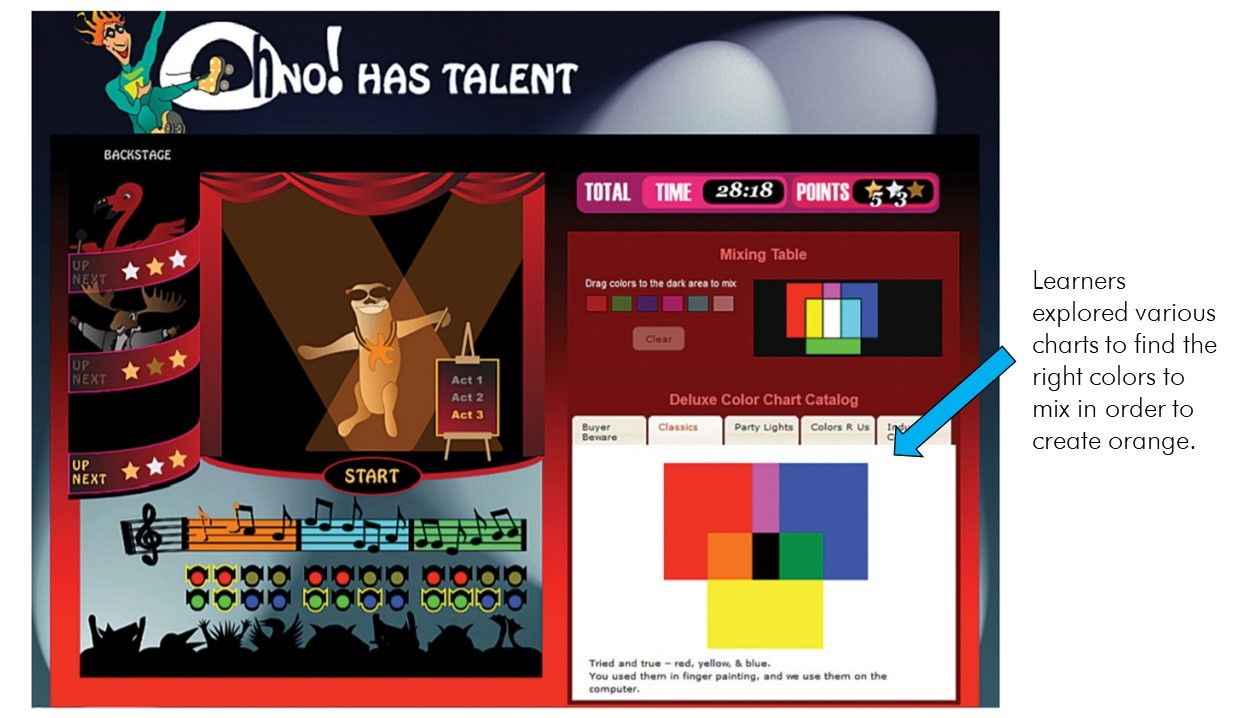
\includegraphics[width=.9\textwidth]{i_figures/choicelet.jpg}
  \caption{Ohno! Has Talent is a choice-based assessment of critical thinking ability where students can explore different charts to decide which ones give the correct information for mixing the intended color (orange). If they create mix the colors correctly, Ohno! will begin singing. Figure adapted from \cite{schwartz2013measuring}.
}
  \label{fig:choicelet}
\end{figure}
%add overlay of figure w/ arrow to point out the learning goal, add in the critical thinking piece for caption. 

One promising avenue for adaptive coaching tools are those that assess motivation and choice. Choice-based assessments and activities examine what choices learners make such as whether they choose to explore resources or try different potential solutions \cite{schwartz2013measuring}. Figure \ref{fig:choicelet} shows an example of a `choicelet' where students can choose to examine a catalog of color mixing charts to determine which charts are correct for their task as an assessment of critical thinking. Much like a human coach, computational coaches could help learners make and evaluate their choices could improve creative learning. In our study with Sh{\"o}wn, we found that some participants in our study wanted to understand more about the reasoning behind suggestions and how the examples could apply to their own comics (Section \ref{sec:shown_exp}). In addition to presenting suggested considerations, adaptive systems like Sh{\"o}wn could also provide explanations for why those considerations might improve a user's work. Many creativity support systems have toolbars that give users a variety of options of tools to user to execute their goals. What if coaching systems had ``strategy bars'' that allowed users to select different high-level strategies to use? This approach would give users a way to quickly explore different methods of achieving their goals and finding the strategy that works best for them.

Good coaches are few and far between, but the benefits of a coach are immeasurable. Issues of access and opportunity prevent some from even being able to afford to pursue their creative desires. Computational support tools could scale the talent of valuable coaches to nearly anyone who wants to learn. I believe that computational coaching tools should give opportunities to explore and connect exploration to their ultimate outcomes, meeting people where they are and helping them define and achieve their goals. I don't think computers should replace people's creativity, nor do I think they can. Rather, I see computational tools as a way of broadening people's horizons so they can accomplish more than they believe is possible.

\section{Closing Remarks}
Our information-driven society comprises an abundance of uncertainty, ambiguity, and information, in which we can often get lost in the woods. It is increasingly tempting to “cool” too soon, settling on
what little certainty we can find. Without “seeing the forest for the trees,” we may never come upon innovative solutions for our most complex problems. My dissertation introduces three strategies that help overcome this challenge. It contributes three interactive and contextual tools that embody these strategies to adaptively scaffold exploration at different stages of the creative process. It provides empirical evaluations and observations to demonstrate the efficacy of these strategies. Finally, the strategies introduced in this dissertation provide direction for open questions of fostering creative learning and scaling computational coaching to catalyze creativity for all. 
Ultimately, I envision a future in which our pedagogy and support tools empower people to practice everyday creativity to achieve their goals and expand human ambition.

%how do computational coaches mix w/ backwards design
%worth considering dual-ended search (how keen am i? how bad do i need to know it?), do convolution of those 2 things.
%socio-emotional factors, one challenge for forest for trees challenge is flying too high (icarus vs. fear of icarus), especially when collaborative (hard to figure out how to give and receive constructive criticism), pulling the plug on something.


% A common strategy here is to include files for each of the chapters. I.e.,
% Place the chapters is separate files: 
%   chapter1.tex, chapter2.tex
% Then use the commands:
%   \include{chapter1}
%   \include{chapter2}
%
% Of course, if you prefer, you can just start with
%   \chapter{My First Chapter Name}
% and start typing away.  

% \subsection{A Figure Example}
% \label{ssec:figure_example}

% \begin{figure}[h] 
%   \centering
%   \includegraphics[width=0.5\textwidth]{sandiego}
%   \caption[A picture of San Diego. Short figure caption must be \protect{$< 4$} lines in the list of figures]
% {A picture of San Diego.  Short figure caption must be \protect{$< 4$} lines in the list of figures and match the start of the main figure caption verbatim. Note that figures must be on their own line (no neighboring text) and captions must be single-spaced and appear \protect\textit{below} the figure.  Captions can be as long as you want, but if they are longer than 4 lines in the list of figures, you must provide a short figure caption.\index{SanDiego}}
%   \label{fig:sandiego}
% \end{figure}

% \subsection{A Table Example}

% While in Section \ref{ssec:figure_example} Figure \ref{fig:sandiego} we had a majestic figure, here we provide a crazy table example.


%%%% TABLE 1 %%%%
% \vspace{0.25in}
% \begin{table}[!ht]
% \caption[A table of when I get hungry.  Short table caption must be \protect{$< 4$} lines in the list of tables]{A table of when I get hungry. Short table caption must be \protect{$< 4$} lines in the list of tables and match the start of the main table caption verbatim.  Note that tables must be on their own line (no neighboring text) and captions must be single-spaced and appear \protect\textit{above} the table.  Captions can be as long as you want, but if they are longer than 4 lines in the list of figures, you must provide a short figure caption.}

% \vspace{-0.25in}
% \begin{center}
% \begin{tabular}{|p{1in}|p{2in}|p{3in}|}

% \hline
% Time of day & Hunger Level & Preferred Food \\

% \hline
% 8am & high & IHOP (French Toast) \\

% \hline
% noon & medium & Croutons (Tomato Basil Soup \& Granny Smith Chicken Salad) \\

% \hline
% 5pm & high & Bombay Coast (Saag Paneer) or Hi Thai (Pad See Ew) \\

% \hline
% 8pm & medium & Yogurt World (froyo!) \\

% \hline
% \end{tabular}
% \end{center}
% \label{tab:analysis3}
% \end{table}



%% APPENDIX
\appendix



%% END MATTER
% \printindex %% Uncomment to display the index
% \nocite{}  %% Put any references that you want to include in the bib 
%               but haven't cited in the braces.
\bibliographystyle{SIGCHI-Reference-Format}  %% This is just my personal favorite style. 
%                              There are many others.
%\setlength{\bibleftmargin}{0.25in}  % indent each item
%\setlength{\bibindent}{-\bibleftmargin}  % unindent the first line
%\def\baselinestretch{1.0}  % force single spacing
%\setlength{\bibitemsep}{0.16in}  % add extra space between items
\bibliography{references}  %% This looks for the bibliography in template.bib 
%                          which should be formatted as a bibtex file.
%                          and needs to be separately compiled into a bbl file.
\singlespace  %to force bibilography environment to use single spacing for each entry 
              %double spacing between entries remains
\end{document}

